%!BIB program = biber
%!TEX program = pdflatex
% header.tex
\documentclass[a4paper,11pt,twoside,english]{book}
\usepackage[a4paper,left=3.5cm,right=2.5cm,bottom=3.5cm,top=3cm]{geometry}
\usepackage{todonotes}
\usepackage[english]{babel}

%usepackage[pdftex]{graphicx}
\usepackage{amsmath,amssymb}


% Theorem-Umgebungen
\usepackage[amsmath,thmmarks]{ntheorem}

% Korrekte Darstellung der Umlaute
\usepackage[utf8]{inputenc}
\usepackage[T1]{fontenc}

% Algorithmen
\usepackage[plain,chapter]{algorithm}
\usepackage{algorithmic}

\usepackage{enumerate}
\usepackage{acronym}
\usepackage{tcolorbox}
\usepackage{csquotes}
\usepackage[hidelinks]{hyperref}



% Bibtex deutsch
%\usepackage{bibgerm}
\usepackage[citestyle=numeric,bibstyle=alphabetic,backend=biber, backref=true]{biblatex}
\addbibresource{literature.bib}
% URLs
\usepackage{url}

% Caption Packet
\usepackage[margin=0pt,font=small,labelfont=bf]{caption}
% Gliederung einstellen
\setcounter{secnumdepth}{5}
\setcounter{tocdepth}{5}

% Theorem-Optionen %
\theoremseparator{.}
\theoremstyle{change}
\newtheorem{theorem}{Theorem}[section]
\newtheorem{satz}[theorem]{Satz}
\newtheorem{lemma}[theorem]{Lemma}
\newtheorem{korollar}[theorem]{Korollar}
\newtheorem{proposition}[theorem]{Proposition}
% Ohne Numerierung
\theoremstyle{nonumberplain}
\renewtheorem{theorem*}{Theorem}
\renewtheorem{satz*}{Satz}
\renewtheorem{lemma*}{Lemma}
\renewtheorem{korollar*}{Korollar}
\renewtheorem{proposition*}{Proposition}
% Definitionen mit \upshape
\theorembodyfont{\upshape}
\theoremstyle{change}
\newtheorem{definition}[theorem]{Definition}
\theoremstyle{nonumberplain}
\renewtheorem{definition*}{Definition}
% Kursive Schrift
\theoremheaderfont{\itshape}
\newtheorem{notation}{Notation}
\newtheorem{konvention}{Konvention}
\newtheorem{bezeichnung}{Bezeichnung}
\theoremsymbol{\ensuremath{\Box}}
\newtheorem{beweis}{Beweis}
\theoremsymbol{}
\theoremstyle{change}
\theoremheaderfont{\bfseries}
\newtheorem{bemerkung}[theorem]{Bemerkung}
\newtheorem{beobachtung}[theorem]{Beobachtung}
\newtheorem{beispiel}[theorem]{Beispiel}
\newtheorem{problem}{Problem}
\theoremstyle{nonumberplain}
\renewtheorem{bemerkung*}{Bemerkung}
\renewtheorem{beispiel*}{Beispiel}
\renewtheorem{problem*}{Problem}

% Algorithmen anpassen %
\renewcommand{\algorithmicrequire}{\textit{Eingabe:}}
\renewcommand{\algorithmicensure}{\textit{Ausgabe:}}
\floatname{algorithm}{Algorithmus}
\renewcommand{\listalgorithmname}{Algorithmenverzeichnis}
\renewcommand{\algorithmiccomment}[1]{\color{grau}{// #1}}

% Zeilenabstand einstellen %
\renewcommand{\baselinestretch}{1.25}
% Floating-Umgebungen anpassen %
\renewcommand{\topfraction}{0.9}
\renewcommand{\bottomfraction}{0.8}
% Abkuerzungen richtig formatieren %
\usepackage{xspace}
\newcommand{\wrt}{w.r.t.\@\xspace} 
\newcommand{\eg}{e.\nolinebreak[4]\hspace{0.125em}\nolinebreak[4]g.\@\xspace}
\newcommand{\ie}{i.e.\@\xspace}
\newcommand{\dahe}{d.\nolinebreak[4]\hspace{0.125em}h.\nolinebreak[4]\@\xspace}
\newcommand{\etc}{etc.\@\xspace}
\newcommand{\evtl}{evtl.\@\xspace}
\newcommand{\ggf}{ggf.\@\xspace}
\newcommand{\bzgl}{bzgl.\@\xspace}
\newcommand{\so}{s.\nolinebreak[4]\hspace{0.125em}\nolinebreak[4]o.\@\xspace}
\newcommand{\iA}{i.\nolinebreak[4]\hspace{0.125em}\nolinebreak[4]A.\@\xspace}
\newcommand{\sa}{s.\nolinebreak[4]\hspace{0.125em}\nolinebreak[4]a.\@\xspace}
\newcommand{\su}{s.\nolinebreak[4]\hspace{0.125em}\nolinebreak[4]u.\@\xspace}
\newcommand{\ua}{u.\nolinebreak[4]\hspace{0.125em}\nolinebreak[4]a.\@\xspace}
\newcommand{\og}{o.\nolinebreak[4]\hspace{0.125em}\nolinebreak[4]g.\@\xspace}
\newcommand{\oBdA}{o.\nolinebreak[4]\hspace{0.125em}\nolinebreak[4]B.\nolinebreak[4]\hspace{0.125em}d.\nolinebreak[4]\hspace{0.125em}A.\@\xspace}
\newcommand{\OBdA}{O.\nolinebreak[4]\hspace{0.125em}\nolinebreak[4]B.\nolinebreak[4]\hspace{0.125em}d.\nolinebreak[4]\hspace{0.125em}A.\@\xspace}
\newcommand{\norm}[1]{\left\lVert#1\right\rVert}
\newcommand{\abs}[1]{\lvert#1\rvert}
\newcommand{\independent}{\protect\mathpalette{\protect\independenT}{\perp}}
\def\independenT#1#2{\mathrel{\rlap{$#1#2$}\mkern2mu{#1#2}}}

\newtcolorbox[auto counter, number within=section, number freestyle={\noexpand\thechapter.\noexpand\arabic{\tcbcounter}}]{threm}[2][]
{
  colframe = tuorange!40,
  colback  = tuorange!20,
  coltitle = tuorange!20!black,  
  title    = Theorem~\thetcbcounter: {#2},
  #1,
}
\newtcolorbox[auto counter, number within=section, number freestyle={\noexpand\thechapter.\noexpand\arabic{\tcbcounter}}]{example}[2][]
{
  colframe = tugray!40,
  colback  = tugray!20,
  coltitle = tugray!20!black,  
  title    = Example~\thetcbcounter: {#2},
  #1,
}

\newtcolorbox[auto counter, number within=section, number freestyle={\noexpand\thechapter.\noexpand\arabic{\tcbcounter}}]{proof}[2][]
{
  colframe = tugreen!40,
  colback  = tugreen!20,
  coltitle = tugreen!20!black,  
  title    = Proof~\thetcbcounter: {#2},
  #1,
}

\let\vec\mathbf
\newcommand{\vect}[1]{\boldsymbol{#1}}
% Leere Seite ohne Seitennummer, naechste Seite rechts
\newcommand{\blankpage}{
 \clearpage{\pagestyle{empty}\cleardoublepage}
}
% Keine einzelnen Zeilen beim Anfang eines Abschnitts (Schusterjungen)
\clubpenalty = 10000
% Keine einzelnen Zeilen am Ende eines Abschnitts (Hurenkinder)
\widowpenalty = 10000 \displaywidowpenalty = 10000
% EOF

% color palette by Erich Schubert https://bitbucket.org/ls8-tudo/beamer-erich/src/template/
\xdefinecolor{tugreen}{RGB}{132, 184, 24} % source: official
\xdefinecolor{tudarkgreen}{RGB}{100, 150, 0} % source: official (purpose: web design)
\xdefinecolor{tulightgreen}{RGB}{224, 234, 204} % source: official (purpose: web design)
\xdefinecolor{tugray}{RGB}{207, 208, 210} % source: Powerpoint template diagram
\xdefinecolor{tugraybg}{RGB}{178, 179, 204} % source: official (purpose: web design)
\xdefinecolor{tuorange}{RGB}{227, 105, 19} % source: another template
\xdefinecolor{tuyellow}{RGB}{242, 189, 0} % source: another template
\xdefinecolor{tucitron}{RGB}{249, 219, 0} % source: another template
\xdefinecolor{tublue}{RGB}{46, 134, 171} % source: imaginary
\xdefinecolor{tudarkblue}{RGB}{30, 89, 114} % source: imaginary
\xdefinecolor{tuviolet}{RGB}{61, 52, 139} % source: imaginary
\xdefinecolor{tumagenta}{RGB}{139, 52, 88} % source: imaginary
\xdefinecolor{tudarkergreen}{RGB}{75, 98, 44} % source: Stefan Michaelis
\xdefinecolor{tuolive}{RGB}{83, 145, 45} % source: Stefan Michaelis
\xdefinecolor{tulime}{RGB}{215, 215, 0} % source: Stefan Michaelis
\xdefinecolor{tugraygreen}{RGB}{217,233,229} % source: Stefan Michaelis
\input{test.tex}
\begin{document}
    \begin{titlepage}
\definecolor{TUGreen}{rgb}{0.517,0.721,0.094}
\vspace*{-2cm}
\newlength{\links}
\setlength{\links}{-1.5cm}
\sffamily
\hspace*{\links}
\begin{minipage}{12.5cm}

\includegraphics[width=8cm]{bilder/tud_logo_rgb}
%\hspace*{-0.25cm} \textbf{TECHNISCHE UNIVERSIT"AT DORTMUND}\\
%\hspace*{-1.2cm} \rule{5mm}{5mm} \hspace*{0.1cm} FACHBEREICH INFORMATIK\\
\end{minipage}

\vspace*{4cm}

\hspace*{\links}
\hspace*{-0.2cm}
\begin{minipage}{9cm}
\large
\begin{center}
{\Large Master's Thesis} \\
\vspace*{1cm}
\textbf{Aggregation Mechanisms for Distributed Exponential Family Models} \\
\vspace*{1cm}
Danny Heinrich\\
% \vspace*{1cm}
June 2020
\end{center}
\end{minipage}
\normalsize
\vspace*{5.5cm}

% \hspace*{\links}

\vspace*{2.1cm}

\hspace*{\links}
\begin{minipage}[b]{5cm}
% \normalsize
\raggedright
Supervisor: \\
Prof. Dr. Katharina Morik \\
Dr. Nico Piatkowski \\
\end{minipage}

\vspace*{2.5cm}
\hspace*{\links}
\begin{minipage}[b]{8cm}
% \normalsize
\raggedright
TU Dortmund Univerity \\
Fakult\"at f\"ur Informatik\\
Künstliche Intelligenz (VIII)\\
https://www-ai.cs.tu-dortmund.de/
\end{minipage}
%%%%%%%%%%%%%%%%%%%%%%%%%%%%%%%%%%%%%%%%%%%%%%%%%%
% bei Kooperation mit anderen Lehrstuehlen,
% sonst weglassen
%\begin{minipage}[b]{8cm}
% \normalsize
%\raggedleft
%In Kooperation mit:\\
%Fakult"atsname\\
%Lehrstuhl-/Institutsbezeichnung
%\end{minipage}
%%%%%%%%%%%%%%%%%%%%%%%%%%%%%%%%%%%%%%%%%%%%%%%%%%

\end{titlepage}

    \tableofcontents
    
    % einleitung.tex
\chapter{Introduction}
With an increasing number of devices and thus data collected on these devices the task of machine learning becomes increasingly difficult.
While the best case scenario in terms of model quality is transferring the data to a central node and then training models on the complete and ever increasing data it is in practice not feasible to do so.
One would incur a large communication overhead by sending the raw data to a central node. 
Doing this for all applications would generally break the communication system. 
Another concern is the need for privacy. We usually do not want to and should not concede our data to central servers.
Even anonymized data can be profiled and tracked back to certain users [TODO CITE].
Therefore, we want to apply machine learning on edge.
Using the devices itself to learn models and then convergecasting some metadata to a central node such a model parameters.
This requires several things, such as energy efficient computing while having limited processing power available.
Furthermore memory and disk-space are also limited especially in the context of mobile or sensor devices.
We propose an aggregation scheme for a distributed or federated learning system. [TODO FEDERATED vs. DISTRIBUTED?]

\section{Motivation and Background}
Communication between devices is inefficient.
Local Models usually have a large variance between each other on the same data/distribution.
Two staple methods, ensembling and aggregation.
Ensembling aims to decide the label of a class by accounting for each decision on the local models e.g. majority vote.
Aggregation aims to aggregate the approximated function, i.e., its parameters to create a new aggregated model, which then predicts the labels.
After aggregation we only need to predict once and not on every local model.
Models introduce non-linearity, which in turn might introduce an error in the aggregation as e.g. averaging is a linear operation.
Model aggregation has been studied by several people.
Aggregation requires communication between local models in a non-centralized approach or communication between local nodes and a coordinator (Federated learning).

Several problems are associated with distributed learning:
Amount of communication required.
Stopping criteria for local models, i.e., when are models close enough to stop training and this includes the question of sample complexity.
Model aggregation itself.

%Eine Referenz~\cite{AggarwalV88}.
\section{Related Work}
Related Work for Model Aggregation, Local Thresholding(Ran Wolff, Assaf Schuster, Michael Kamp), Sample Complexity , Communication effieciency.


Motivation for this topic, why do we need distributed learning or even resource constrained ?

The related work to this thesis divides itself upon several reserach areas. 
For one we have the general approach to model aggregation and specifically in the distributed setting.
Then we have to consider the sample complexity, i.e., having a general idea bout how much data we need on each device.
This can be done by using a general network approach or using existing bounds such as the hoefding bound to guarentee the models being somewhat close.

What as already been done ?
Naive Kullback Leibler Aggregation with Bootstrapping, Radon Machines for Model Ensembling, simple averaging.

What guarentees do we have ? 
hoefding Bound, Regret etc.
\section{Thesis Structure}
    % kapitel2.tex
\chapter{Background}
\label{chapter:kap2}

\section{Notation}
\label{sec:nota}
Let us first define our notation. 
Random Variables will be noted as $X$ and vectors will be written in bold letters, e.g. a vector of random variables $\vect{X} = \{X_1, X_2, \ldots, X_m\} \in \mathbb{R}^m$.
The state space of a random variable will be denoted as a cursive letter of that random variable $\mathcal{X}$ and the statespace for  a random vector likewise as $\vect{\mathcal{X}}$.
Parameters of a probability density function in the context of the canocical exponential family will usually be noted as $\vect{\theta} \in \mathbb{R}^n, \quad \mathbb{N}^+$.
Here $\mathbb{N}^+$ is defined as $ \mathbb{N}^+ = \mathbb{N} \setminus \{0\}$.
Model parameters on the i$^{th}$ local device will be noted as $\vect{\theta^i}$, while $\vect{\theta_i}$ is the entry at the i$^{th}$ position of the parameter vector.
A multivariate gaussian normal distribution for example has parameters of the form $\vect{\theta} = (\vect{\mu}, \vect{\Sigma})$, with mean $\vect{\mu} \in \mathbb{R}^{n}$ and covariance matrix $\vect{\Sigma} \in \mathbb{R}^{n \times n}$.
Additional notations for model parameters will be introduced if necesesary.
\todo{More generally any variable denothed with \* is optimal, \^ is global and \~ is local}
In the context of optimization and optimality we assume $\vect{\theta}^*$ to be the true, unknown parameter vector.
The global parameters vectors, i.e., the parameters obtained by a global model, which has access to all available data is denoted as  $\vect{\hat{\theta}}$.
Finally, $\vect{\tilde{\theta}}$ denotes any local parameter vector and $\vect{\tilde{\theta}}^{(i)}$ the i$^{th}$ local parameter vector respectively.


\section{Probability Theory}
This is the Bayes Theorem:
\begin{equation}
    P (A \lvert B) = \frac{P(B \lvert A) \cdot P(A)}{P(B)}
\end{equation}


\section{Exponential Families}
\label{sec:expf}

We will now introduce a convenient property of parameters from canonical exponential families, asymptotic normality of the maximum likelihood estimator. 

The canonical exponential family is defined as 
\begin{equation}
    p(\vect{x} \lvert \vect{\theta}) = \frac{1}{Z(\vect{\theta})} \prod_{c \in \mathcal{C}} \psi_c(\vect{x})
\end{equation}

\subsection{Asymptotic Normality}
\label{ssec:asymp}
The Maximum Likelihood Estimator of canonical exponential families is consistent, regular and thus asymptotic normal i.e. $\sqrt{n}(\theta - \theta^*) \sim \mathcal{N}(0, i(\theta^*)^{-1})$.
Implying, that the paremeters follow a normal distribution with the  true parameter vector as mean an the inverse fisher information as covariance, with 

\begin{equation}
    i(\theta^*) = \frac{\partial}{\partial^2 \vect{\theta}} p(x \lvert \vect{\theta})
\end{equation}

being the fisher information matrix.

We can interpret this result in such way that a set of parameter vectors obtained from data sets $\{\mathcal{D}_1, \ldots \mathcal{D}_n\}$ is normally distributed around the true parameter vector for a sample size of $n \leftarrow \infty$. 
This in turn implies that we can treat parameter vectors of local devices as samples from such a distribution and use this to estimate the maximum likelihood of the parameter space.
Addtionally we can use some $\vect{\theta}$ and assume this to be $\theta^*$ and use the result for sampling additional models.


\section{Probabilistic Graphical Models}
\label{sec:pgm}
When dealing with statistical (bayesian) models our goal usually is to estimate a set of parameters of a predetermined distribution that reduces the risk of predicting the wrong outcome (Risk Minimization). 
This is usually done by maximizing the Likelihood of the parameters having generated the data set $\mathcal{D}$ (see \ref{ssec:train}).

Let $\vect{X}$ be a random vector as defined in secition \ref{sec:nota}. 
Each entry in $X_i \in \vect{X}$ corresponds to a single random variable.
The most simple statistical models model each random variable individually while not accounting for dependencies between two or more variables.
This leads to worse estimates as the model can not capture the full scope of the underlying distribution.
With Probabilistic Graphical Models we can capture the underlying dependencies between these random variables in order to create a better estimate for the assumed distribution $\mathcal{D}$ adheres to.

When estimating parameters of a distribution we may consider each feature a random variable and the data generated a result of a stochastic process based on this random variables.
Probabilistic Graphical Models (PGM) are a powerful tool to model conditional independencies between random variables. 
We express each random variable as a node in a graph and each edge between two nodes represents a dependency. 
With the exception of trees and graphs with bounded treewidth performing exact inference in such a Graph is NP-Hard.
This is a result from having to compute the marginal distribution, i.e., summing over all possible states of all maximum cliques inside the graph.
However, methods exist, such as loopy belief propagation to perform approximate inference.
We may also apply a junction tree algorithm to transform the graph into a tree, where exact inference is possible in polynomial time.

When considering probabilistic graphical models we usually utilize parametric distributions, that are part of the exponential family. 
Our goal is to estimate the parameters of such a distribution, which optimizes some criterion e.g. Maximum Likelihood or Maximum Entropy.


After estimating the parameters for each distribution and device, we employ an aggregation mechanic to create a composite model.
Distributed integer probabilistic graphical models \cite{piatkowski2019distributed} have recently been considered by Piatkowski.
In this specific scenario the models were aggregated using the average over all local models.
Other existing aggregation mechanics are discussed in section.
Additionally we need to define a stopping criterion where every device will stop sending messages to other devices, which means we require some kind of convergence.
This is usually the case when most devices have a similar local model.
In the following we will consider existing work on that specific research area and then lay out the necessary steps and challenges for the thesis.

Probabilistic Graphical Models are usually represented as a Graph, i.e., a set of vertices and edges that represent the independency structure of $\vect{X}$.
Each vertex corresponds to a random variable and each edge is a dependency between two variables.
Formally, let $G = (\vect{X},E)$ be a Graph with $\vect{X} =\{X_1 \ldots, X_n\}$, $\vect{\mathcal{X}} = \{\mathcal{X}_1, \ldots, \mathcal{X}_n\}$ and $E \subseteq \vect{X} \times \vect{X}$

\subsection{Markov Random Fields}

A Markov Random Field is a probabilistic graphical model to represent the joint probability of a random vector $\vect{X}$. 
Given a set of special properties, the Markov Properties we can express the joint probability distribution in terms of cliques in the graph.

\subsubsection*{Markov Properties}
Probabilistic graphical models are considered Markov Random Fields if the Graph is undirected and the three markov properties hold for any set of random variables indexed by the vertices of G $\vect{X} = \{X_v\}, v \in V$

\paragraph*{Pairwise Makrov Property}
\paragraph*{Local Markov Property}
Given a random variable $X_v$ it is independent of all other variables given its neighbours 
$X_v \independent X_{V\setminus (v \cup \mathcal{N}(v))} \lvert X_{\mathcal{N}(v)}$
\paragraph*{Global Makrov Property}

\paragraph*{}
\paragraph*{Clique Factorization}

A clique is a subset of nodes $C \subseteq V$ such that, $\forall u,v,  \in C, u \neq v: \exists (u,v) \in E$ there exists and edge in $E$ for all nodes in $C$, i.e., the subset is fully connected.
Now let $\mathcal{C}$ be set set of maximal cliques, i.e., the set of cliques that are not included in any other clique or formally 
\begin{equation}
    \forall C_i, C_j \in \mathcal{C}, i \neq j  : C_i \not\subset C_j, C_j \not\subset C_i, C_i \neq C_j
\end{equation}
there exists no such pair of cliques in $\mathcal{C}$ such that either one is a true subset or the other.
This is not to be confused with the maximum clique, which is the largest clique of the graph $G$, i.e. $\max \mathcal{C} = \max \{\abs{\mathcal{C_1}}, \ldots, \abs{C_n}\}$ the clique with maximum cardinality.

We can then express the joint probability distribution in terms of the set of maximal cliques, by treating each clique as a local probability density function and then factorizing over all maximal cliques. 
We assign a potential function $\psi_C: \mathcal{X}_C \leftarrow \mathbb{R}$ to the clique that maps any state of the clique $\vect{x}_C \in \mathcal{X}_C$ to a positive real valued number.
The clique factorization is then defined as:

\begin{equation}
    \mathbb{P}(\vect{X}=\vect{x}) = \frac{1}{Z} \cdot \prod_{C \in \mathcal{C}} \psi_C(\vect{x}_C)
\end{equation},
where $Z$ is the normalizer of the probability density function, $\mathbb{P}$ is a probability density function, i.e.:

\begin{equation}
    \sum_{\vect{x}\in \mathcal{\vect{X}}}   \frac{1}{Z} \prod_{C \in \mathcal{C}} \psi_C(\vect{x}_C)  = 1.
\end{equation}

The partition function $Z$ is therefore defined as sum over factorizions over all possible states:
\begin{equation}
    Z = \sum_{x\in \mathcal{X}} \prod_{C \in \mathcal{C}} \psi_C(\vect{x}_C)
\end{equation}

\begin{equation}
    \psi_C(\vect{x}_c) = \exp(\sum_{i=1}^n \theta_i \cdot \phi(\vect{x})_i)
\end{equation}

\paragraph*{Exponential Families}

\subsubsection{Structure Learning}
    Determining the Structure for the graph is important as we want to model the actual dependencie
    between random variables. 
    We may decide to drop dependencies in order to simplify the model, which allows for faster and exact training(in case the graph is a tree).
    
    We will use the Chow-Liu algorithm to approximate a independency structure, which always results in a tree.
    The algorithm computes the cross entropy for every pair of nodes and then computing the minimum spanning tree to 
    obtain the edges with the largest correlation.
    This limits the clique size in the graph to two, resulting in a tree, but also limiting the number of nodes that depend on each other.

    In this work the Chow-Liu algorithm is used for all independency structure approximations.
\subsection{Training}
\label{ssec:train}

Exponential Family is family of parametrized densities
Parameters have to be estimated
Maximum Likelihood Estimation
Given Data maximize Likelihood of Data being generated by distribution
Maximization over Distribution Parameters 
Negative Average Log Likelihood to prevent numerical errors
In general no closed form solution
Derivative is average sufficient statistics + expectation of $\vect{X}$
Log Partition is P-Complete, however solvable in poly time for trees.

optimization via Belief Propagation -> Inference
\subsection{Inference}
\label{ssec:inf}

Computing Clique Marginals
Belief Propagation
Exact for Trees 
Loopy Belief Propagation for non-tree Graphs

Since we are using the Chow-Lio algorithm to approximate the independency structure it is sufficient to use Belief Propagation for inference as this is guaranteed to be optimal and deterministic on trees.

\section{Distributed Learning}
There are mainly two different architectural approaches to distributed learning. 
The first approach is a decentralized approach without coordinator.
Communication between nodes is allowed and necessary to transmit some amount of data to reach an overall conclusion to the learning task.
The other approach involves a centralised coordinator node that broadcasts intermediate results or correction terms to local nodes.
The nodes in this approach send their data to the coordinator. 
Hybrid-Methods, where both types of architerure are mixed are also possible.
This work will focus on the second type, while also giving some theoretical insights to the decentralized approach.

Moreover the data may be horizontally or vertically distributed, i.e., either all features are available on each device, but only a small portion of the data or each device has access to all data of a subset of features.
Sensor Networks are an example for the latter, where each sensor may only generate one or more features such as temperature or magnetic field strength.

The key questions we have to ask ourselves in a distributed settting with horizontally distributed data are:
\begin{itemize}
    \item How much data is sufficient to obtain a proper estimate for the model on each device ? 
    \item When, how much and what do we communicate either between local devices or the coordinator ?
    \item What are we allowed to communicate ? (in terms of privacy preservation on user devices)
\end{itemize}

Depending on the task we may have to restrict communication, memory and processor consumption to an absolute minimum.
Here, statistical models have one major advantage over other models, that is they require less disk space to store and process as only certain statistics need to be preserved.
These are generally the parameters of the distribution we provide.
With markov random fields using a probability distribution from the exponential family we do not even have to store the data in memory has we only have to preserve the sufficient statistics for training and inference.

The two major issues we have to deal with are therefore the sample complexity and the model aggregation.
As the main focus of this work is the model aggregation, which will be featured in chapter \ref{chapter:ch3}, we will now briefly discuss sample complexity.

\subsection{Sample Complexity}
One of the key questions of distributed learning is the number of samples required to obtain local models that are sufficiently good, i.e., when to stop learning and either start communication with the coordinator
or to terminate the algorithm and produce a final aggregate model. 
The problem to find the number of samples required is known to be hard \todo{cite} and as such no exacty solution to this problem exists.
However, an upper bound on the sample complexity is given by the Hoefding-Bound. 
We apply the Hoefding-Inequality on the pairwise difference between average sufficient statistics of local models.

The Hoefding-Inequality is given by
\begin{equation}
    P(\vect{\bar{X}} - \mathbb{E}[\vect{\bar{X}}] \geq t ) \leq \exp^{-2\abs{\mathcal{D}]t^2}},
\end{equation}

where for some constant $t$ the probability of the difference between the empirical mean of a random variable and its expectation is begin greater than $t$ is negatively exponential bounded by the amount of data seen.

It can be shown that for $t = \frac{\sqrt{(c+1) \log d}}{2\abs{\mathcal{D}}}$ the difference between two average sufficient statistics $\vect{\mu}^i = \frac{1}{\mathcal{D}_i} \sum_{x \in \mathcal{D}} \vect{\phi(x)}, \quad \vect{\phi(x)} \in \mathbb{R}^d$ of a probabilistic graphical model is bounded by
\begin{equation}
    \norm{\mu^{i} -  \mu^{j}}_\infty \leq 2 \sqrt{
        \frac{(c+1) \log d}
        {2\abs{\mathcal{D^{'}}}}
        } = \epsilon
\end{equation},
with probability of at least $\delta= (1- 2 \exp(-c \log d))$. Here $D^{'} = \min(\abs{\mathcal{D}^i}, \abs{\mathcal{D}^j})$.
The proof is provided by Piatkowski \cite{piatkowski2019distributed}. \todo{Maybe put this in appendix}
Addtionally, as the average sufficient statistics approach each other so do the model parameters to some degree as shown by \todo{CITE}.

As the model parameters approach each other, we can show by Popoviciu's Theorem \cite{popoviciu1935equations} 
\begin{threm}{Upper Bound on the Variance}
    Let $\vect{X}$ be a bounded random variable with $\inf(\vect{X}) = b$ and $\sup(\vect{X}) = a$, 
    then the variance $\sigma^2$ is bounded by 
    \begin{equation}
        \sigma^2 \leq \bigg(\frac{a-b}{2}\bigg)^{2}
    \end{equation}
\end{threm}

For the interested reader we refer to Sharma et al. \cite{sharma2010betterbounds} for more information about upper and lower bounds for variances.

\begin{proof}{Bound of Variances}

Let $f(t) = \mathbb{E}[(\vect{X} - t)^2]$ for some $t$ and $b = \inf(\vect{X})$, $a = \sup(\vect{X})$ for a bounded random variable $\vect{X}$.

The derivative of $f(t)$ is:
\begin{equation*}
    \begin{split}
        f'(t) &= \frac{d}{dt} \mathbb{E}[(\vect{X} - t)^2]\\ 
            &= -2\mathbb{E}[\vect{X}] + 2t = 0\\
    \end{split}
\end{equation*}
and takes its minimum at $t = \mathbb{E}[X]$, which is $f(\mathbb{E}[X]) = \mathbb{E}[(\vect{X} - \mathbb{E}[X])^2] = Var[X]$ the variance of the random variable.

Now let  $t=\frac{a-b}{2}$, the arithmetic mean $\sup(\vect{X})$ and $\inf(\vect{X})$, which maximizes the distance between $t$ and $a,b$.
We obtain the following inequalities for the maximizer:

\begin{equation*}
    Var[\vect{X}] = f(\mathbb{E}[\vect{X}]) = \mathbb{E}[(\vect{X} - \mathbb{E}[\vect{X}])^2) \leq f(\frac{a-b}{2})
\end{equation*}

with 

\begin{equation*}
    f\bigg(\frac{a-b}{2}\bigg) = \mathbb{E}\bigg[\bigg(\vect{X} - \frac{a-b}{2} \bigg)^2\bigg]= \frac{1}{4} \cdot \mathbb{E}\bigg[\big((\vect{X} - b) + (\vect{X} - a)  \big)^2\bigg]
\end{equation*}

We then have 
\begin{equation*}
         \bigg((\vect{X} - b) + (\vect{X} - a)  \bigg)^2 \leq  \bigg((\vect{X} - b) - (\vect{X} - a)  \bigg)^2  = (a-b)^2 
\end{equation*}
We now show that the equality on the right hand side holds.
Let $\vect{X} = a - \epsilon, \quad \epsilon \in [b,a]$ : 

\begin{equation*}
    \begin{split}
        \bigg(((a-\epsilon) - b) - ((a-\epsilon) - a)  \bigg)^2  &=  (a-b)^2\\
        \bigg(((a-\epsilon) - b) + \epsilon  \bigg)^2 &=  (a-b)^2 \\
        (a-b)^2  &= (a-b)^2,\\
    \end{split}
\end{equation*}
\qed
thus for any $\epsilon \in [b,a]$ the equality holds.

For the expected value of $\vect{X}$ we then have
\begin{equation*}
    \frac{1}{4} \cdot \mathbb{E}\bigg[\big((\vect{X} - b) + (\vect{X} - a)  \big)^2\bigg] \leq \frac{1}{4} \cdot \mathbb{E}\bigg[\big((\vect{X} - b) - (\vect{X} - a)\big)^2\bigg] = \bigg(\frac{a-b}{2}\bigg)^2,
\end{equation*}\qed
obtaining the following bound on the variance of a bounded random variable:
\begin{equation}
    Var[\vect{X}] = \sigma^2 \leq \bigg(\frac{a-b}{2}\bigg)^2
\end{equation}
\qed
\end{proof}


It follows that
\begin{equation*}
    Var[\vect{X}] \leq f(\frac{a-b}{2}) \leq  \frac{1}{4} \cdot \mathbb{E}\bigg[\big((\vect{X} - b) - (\vect{X} - a)\big)^2\bigg]  =  \bigg(\frac{a-b}{2}\bigg)^2 
\end{equation*}\qed

Recall that $\norm{\vect{\mu}^{i} -  \vect{\mu}^{j}}_\infty \leq  \epsilon$, where $\epsilon$ provides the largest difference between two entries of the average sufficient statistics hence let $a - b = \mu^{i}_k - \mu^{j} = epsilon$.
This means that there exists no larger difference between the two vectors resulting in an upper bound for the variance of the average sufficient statistics with $a - b = \epsilon$ 
\begin{equation*}
    Var[\vect{\mu}^{i}_k -  \vect{\mu}^{j}_k] \leq \frac{\epsilon^2}{4} \quad \forall i,j,k
\end{equation*}.
Given two average sufficient statistics we can employ the Hoefding Bound to guarantee the distance between these two to be smaller than some $\epsilon$ with probability $\delta$


As the amount of data on each device increases we can also measure how close the sufficient statistics are with probability $\delta$ by rearranging the above equation. 
This is the most common scenario in distributed learning. As time goes on the amount of data increases allowing us to continuously measure the distance and variance between the sufficient statistics.
Once we reach our predetermined goal on a device, i.e. $\abs{\mathcal{D}}^^i$ is sufficiently large to satisfy our bound we stop collecting more data send the parameter vector to the coordinator node.

\todo{Equation}

We see that as $\abs{\mathcal{D}}$ increases, for a fixed $\delta$ the distance $\epsilon$ decreases and so does the variance. 

\todo{Maybe Plot eps and delta in 3D}


    % Model_Aggregation.tex

\chapter{Model Aggregation}
\label{chapter:ch3}
Model aggregation is the task of combining a set of models obtained from a group of learners, preserving the original structure and quality, while creating a more well-informed aggregate model.
\begin{definition}[parbox=false]{Model Aggregation}
    Let $\mathcal{H}$ be a space of all feasible solutions for some parametrized machine learning task with given structure and $\mathcal{F}$ be the space of all feasible functions $f: \mathcal{H}^k \rightarrow \mathcal{H}$ that map a set of feasible solutions to a single solution.
    Furthermore, let $\vect{M}$ be a random variable and $\mathcal{M}$ its state space with samples  $\vect{m} = (m^1, \ldots, m^k) \in \mathcal{H}^k$ from the distribution of $\vect{M}$.
    Where a model $m^i$ is a collection of attributes such as parameters or structure information

    Our goal is to find an aggregate function $f \in \mathcal{F}$ such that it minimizes some loss function with a limited amount of samples from the distribution of $\vect{M}$:
    \begin{equation}
        \label{eq:regret}
        \arg\min_{f \in \mathcal{F}} \; d(f(\vect{m}), m^*),
    \end{equation}
    where $m^*$ is the optimal aggregate model and $d: \mathcal{H} \times \mathcal{H} \rightarrow \mathbb{R}$ is some quality measure or distance function.
    Note that we only need to aggregate these elements of $m^i$ that fully characterize the model.
    %Consider statistical models with known structure and distribution. 
    %We only require the parameters in addition to the graph and state-space to perform inference.
\end{definition}

In the context of this work feasible solutions are from a parametrized family of densities, i.e., the solution space $\mathcal{H} = \Theta$ and  $m^i = \vect{\theta}^i \in \mathbb{R}^d$, where $d$ is the number of parameters of the model. 
Note that we restrict models to their parameters only, while they usually contain additional elements such as the sufficient statistics $\tilde{\vect{\mu}}$.

The aggregate function is then $f: \mathbb{R}^{d \times k} \rightarrow \mathbb{R}^{d}$ such that the input is a matrix with $d \times k$ entries, where each column corresponds to a single parameter vector.

For exponential families we already know from  \autoref{ssec:asymp} that $\vect{M} \sim \mathcal{N}(\vect{\theta}^*, i(\vect{\theta}^*)^{-1}/n)$ is asymptotically normal.

Basic approaches to federated learning involve training models on each learner first and afterward sending their models to the coordinator.
\autoref{alg:magg} presents this approach in a federated learning setting. 
Each round, we update the local data sets and use those to estimate the parameters in parallel. 
Afterward, we send the local parameters to the coordinator, which performs the aggregation and convergence-checks.
Note that depending on the stopping criterion, we may need to supply additional information to the coordinator, such as the number of locally observed samples. 
The stopping criterion may also involve the aggregate model or computing some distance function $d: \mathcal{H} \times \mathcal{H}  \rightarrow \mathbb{R}$  to determine whether the training should be stopped.
\begin{algo}{Distributed Model Aggregation}
    \begin{algorithm}[H]
    \caption[Distributed Learning with PGMs]{General approach to distributed learning. While the stopping criterion $C$ has not been fulfilled, the distributed learners update the observed data in each round and train a new or updated model. Afterward, the local parameters are sent to the coordinator and aggregated with some aggregation algorithm.}
        \begin{algorithmic}[1]
            \label{alg:magg}
            \REQUIRE Datasets $\mathcal{\vect{D}} = \{\mathcal{D}_1, \ldots,\: \mathcal{D}_k\}$, Graph $G=(V,\:E)$, States $s \in \mathbb{N}^{\abs{V}}$ and Stopping Criterion C \\
            \ENSURE Aggregate Model $\vect{\tilde{\theta}}$  \\
            \WHILE{not STOP} \STATE{%
            \COMMENT{Train models on each learner in parallel}\\
            \FORALL{Devices $i = 1, \ldots, k$} 
            \STATE{
                $\mathcal{D}_i \leftarrow \text{update}(\mathcal{D}_i)$ \\
                $\vect{\theta}^{(i)} \leftarrow \text{train}(\mathcal{D}_i,\: G,\: s)$\\
                $\text{send}(\vect{\theta}^{(i)})$\\
            } 
            \ENDFOR
            }\\
            \COMMENT{On the Coordinator} \\
            \STATE{$\vect{\tilde{\theta}} \leftarrow \text{aggregate}((\vect{\theta}^{(1)},\ldots,\: \vect{\theta}^{(k)}))$}\\
            \IF{C is fulfilled}
                \STATE{Broadcast STOP} \\
            \ENDIF
            \ENDWHILE
            %\IF{<condition>} \STATE {<text>} \ELSE \STATE{<text>} \ENDIF
            %\IF{<condition>} \STATE {<text>} \ELSIF{<condition>} \STATE{<text>} \ENDIF
            %\FOR{<condition>} \STATE {<text>} \ENDFOR
            %\FOR{<condition> \TO <condition> } \STATE {<text>} \ENDFOR
            %\REPEAT \STATE{<text>} \UNTIL{<condition>}
            %\LOOP \STATE{<text>} \ENDLOOP
            %\AND, \OR, \XOR, \NOT, \TO, \TRUE, \FALSE
            \RETURN {$\vect{\tilde{\theta}}$}
        \end{algorithmic}
    \end{algorithm}
\end{algo}
Some additions to this basic approach may include sending the aggregate back to a subset of learners, which violate some threshold, e.g., local models that are considered as an outlier when compared to the other models.
%Let us now discuss different types of aggregation functions $f \in \mathcal{F}$ that can be used to achieve our goal of aggregating models received from distributed learners.

%\section{Aggregation Mechanisms}
We will now discuss different aggregation methods $f \in \mathcal{F}$, which are represented by line 6 in \autoref{alg:magg}.
The optimal model $m*$ is usually not known and cannot be directly estimated or obtained.
While  $m*$ is unknown, we can still compare different aggregation functions $f$ with each other to determine the most efficient and best-performing aggregator.


\section{Averaging}

Probably the most intuitive approach to aggregate a set of parameters or models is to simply compute the  arithmetic mean of all parameters.
\begin{equation}
    \label{eq:arithmean}
    \hat{\theta} = \frac{1}{k} \sum_{i=1}^k \theta^i
\end{equation}
Recall that in \autoref{ssec:asymp} we showed that the maximum likelihood estimator for canonical exponential families is asymptotically normal.
Hence, each $\vect{\theta}^i$ is one sample from the normal distribution $\vect{\theta}^i \dot{\sim} \mathcal{N}(\vect{\theta}^*, i(\vect{\theta}^*)^{-1}/n)$ around the true parameters and the inverse Fisher information.
We can then perform a maximum likelihood estimation for the parameters of a normal distribution. 
Let $\vect{\theta}^*$ be the mean and $i(\vect{\theta}^*)^n$ be the covariance matrix and any set of $\vect{\theta}$ be the observed data.
We then obtain the following estimator for the mean of the normal distribution.
\begin{proof}{Maximum Likelihood Estimator Normal Distribution}
    For $\mathcal{N}(\vect{\theta}^*, i(\vect{\theta})^{-1}/n)$ the we want to find the maximizer for $\vect{\theta}^*$ for the maximum likelihood estimator. 
    The partial derivative of $\ell$ \wrt $\vect{\theta}^*$ given $\vect{\theta}$ is:
    \begin{equation}
        \begin{split}
        \frac{\partial}{\partial \vect{\theta}^*}&\ell_{\mathcal{N}}(\vect{\theta}^*, \vect{i(\vect{\theta}^*)^{-1}/n}; \vect{m}) =  \frac{\partial}{\partial \vect{\theta}^*} \sum_{\vect{\theta} \in \vect{m}} \log \mathcal{N}(\vect{\theta}; \vect{\theta}^*, \vect{i(\vect{\theta}^*)^{-1}/n})\\
        &=  \sum_{\vect{\theta} \in \vect{m}} \frac{\partial}{\partial \vect{\theta}^*} \log \frac{1}{\sqrt{2 \pi} \abs{i(\vect{\theta}^*)^{-1}/n}} \cdot \exp\bigg(\frac{1}{2} (\vect{\theta} - \vect{\theta}^*)^Ti(\vect{\theta}^*)/n(\vect{\theta} - \vect{\theta}^*) \bigg) \\
        &=  \sum_{\vect{\theta} \in \vect{m}} \frac{\partial}{\partial \vect{\theta}^*} \log (\frac{1}{\sqrt{2 \pi} \abs{i(\vect{\theta}^*)^{-1}/n}}) + \frac{1}{2} (\vect{\theta} - \vect{\theta}^*)^Ti(\vect{\theta}^*)/n(\vect{\theta} - \vect{\theta}^*) \\
        &=  \sum_{\vect{\theta} \in \vect{m}} \frac{\partial}{\partial \vect{\theta}^*} \frac{1}{2} (\vect{\theta} - \vect{\theta}^*)^Ti(\vect{\theta}^*)/n(\vect{\theta} - \vect{\theta}^*) - \log \sqrt{2 \pi} \abs{i(\vect{\theta}^*)^{-1}/n} \\
        &= - \frac{1}{2} i(\vect{\theta}^*)/n \sum_{\vect{\theta} \in \vect{m}} (\vect{\theta} - \vect{\theta}^*) = 0 \\
        &\Leftrightarrow \vect{\theta}^* = \frac{1}{\abs{\vect{m}}} \sum_{\vect{\theta} \in \vect{m}}  \vect{\theta}
        \end{split}
    \end{equation}
\end{proof}
Thus the arithmetic mean maximizes the likelihood of a normal distribution.

This result already implies that asymptotically the arithmetic mean acts as the proper maximum likelihood estimator for the actual distribution. 
However, this only applies in the asymptotic case. 
As such, we want to explore ways to obtain better aggregates, especially when we only have a small sample size or models with high variance.

\section{Weighted Averaging}
In case we do not have a sufficient amount of samples to perform model averaging, we have to find an alternative to the arithmetic mean aggregation. 
When the sample size is small, we possibly observe models that have a comparably low likelihood of being observed, i.e., the observed models have high variance. 
The importance of these models is then overestimated since all local models contribute equally to the model average leading to overall worse aggregates.
With the weighted arithmetic mean, we introduce weights $\vect{\lambda}$ assigning some measure of importance to a local model. 
Models with a larger weight contribute more to the aggregate, while the ones with smaller weights contribute less.
Additionally we normalize the weights such that $\sum_{i=1}^k \lambda_i = 1, \lambda_i \geq 0$, i.e., the elements sum to one, which represents prior distribution over $\vect{\theta}^i$, where $\mathbb{P}(\vect{M} = \vect{\theta}^i) = \lambda_i$ for a finite set $\vect{m} = \{\vect{\theta}^1, \ldots, \vect{\theta}^k\} \subset \mathcal{M}$ of parameter samples from the probability distribution over $\vect{M}$.

Then, instead of computing the arithmetic mean, which assumes all weights to be equal to $1$, we compute
\begin{equation}
     \hat{\vect{\theta}} = \sum_{i=1}^k \lambda_i \theta^i = \tilde{\mathbb{E}}_{\vect{m}}[\vect{M}],
\end{equation}
which is the empirical expected value of $\vect{M}$ if and only if $\vect{\lambda}$ is a probability measure.
Obtaining these weights is a challenging task as this requires prior knowledge about each local model or the distribution of local models.
We may consider evaluating each model using a performance metric or scoring function and use the normalized scores as means to obtain $\vect{\lambda}$
\begin{equation}
    \lambda_i = \frac{\log f(\vect{\theta}^i)}{\sum_{j=1}^k \log f(\vect{\theta}^j)},
\end{equation}
where $f: \mathbb{R}^d \rightarrow \mathbb{R}_+$ is an arbitrary positive real valued function, that maps each local model to some score, probability or likelihood.

Now let $f(\vect{\theta}^i) = \log \mathcal{N}(\vect{\theta}^i \lvert \vect{\mu}, \vect{\Sigma})$ be the likelihood function of a secondary normal distribution.
Each weight is then given by
\begin{equation}
    \label{eq:normll}
    \lambda_i = \frac{\log \frac{1}{\sqrt{2\pi\lvert \vect{\Sigma} \rvert}} \cdot \exp^{-\frac{1}{2} \cdot (\vect{\theta}^i - \vect{\mu})^T\vect{\Sigma}^{-1}(\vect{\theta}^i - \vect{\mu})}}{\sum_{j=1}^k \log \frac{1}{\sqrt{2\pi\lvert \vect{\Sigma} \rvert}} \cdot \exp^{-\frac{1}{2} \cdot (\vect{\theta^j} - \vect{\mu})^T\vect{\Sigma}^{-1}(\vect{\theta^j} - \vect{\mu})}},
\end{equation}
which are the normalized weights based on all known local models.
Intuitively, this measures the likelihood of each model based on some additional information such as expert knowledge.

Given that the actual distribution of $\vect{\theta}$ is known, we can simply use the complete MAP-Estimator, as this allows us to include prior information about the parameter distribution.

\subsection{MAP Estimator}
When dealing with likelihood optimization, we usually assume the prior probability to be constant; that is, we treat all possible parameters as equally likely.
The Maximum a-Posteriori(MAP)-Estimator includes the prior information such that we assume the parameters to follow some probability distribution.
Including expert knowledge is particularly useful in settings where data is scarce.
However, if the underlying assumption of the prior's distribution does not hold, they dominate the estimator resulting in worse models.
Recall that we obtain the posterior probability for a set of local models $\mathcal{M}$ as the product of likelihood and prior
\begin{equation}
    \begin{split}
    \arg\max_{\vect{\theta}}\mathbb{P}(\vect{\theta} \lvert \mathcal{M} ) &= \arg\max_{\vect{\theta}} \frac{\mathbb{P}(\mathcal{M}\lvert \vect{\theta}) \mathbb{P}(\vect{\theta}) }{\mathbb{P}(\mathcal{M})} \\
    &\propto  \arg\max_{\vect{\theta}}\mathbb{P}(\mathcal{M}\lvert \vect{\theta}) \mathbb{P}(\vect{\theta})  ,
    \end{split}
\end{equation}
where the denominator does not change the optimum \wrt $\vect{\theta}$ and can, therefore, be omitted.

Given a normal distributed prior for $\vect{\theta}$, we can  compute the MAP-estimate as the weighted average of the prior and the MLE-Estimate for the mean:
\begin{equation}
    \label{eq:mapest}
    \begin{split}
    \arg\max_{\vect{\theta}} \ell(\vect{\theta}; \mathcal{M}, \vect{\lambda}) &= \arg\max_{\vect{\theta}} \sum_{i=1}^k \log \mathbb{P}(\mathcal{M}\lvert \vect{\theta}) \mathbb{P}(\vect{\theta}) \\
    &= \arg\max_{\vect{\theta}} \sum_{i=1}^k   \log \mathcal{N}(\vect{\theta}; \vect{\theta}^*, i(\vect{\theta}^{-1}/n))+  \log \mathcal{N}(\vect{\theta}^i ; \vect{\theta}, \Sigma).
    \end{split}
\end{equation}
Taking the derivative of \autoref{eq:mapest} \wrt $\vect{\theta}$ we get
\begin{equation}
    \vect{\theta} = \frac{\vect{\theta}^*  + n \cdot \Sigma \cdot i(\vect{\theta}^*) \sum_{i=1}^k \vect{\theta}^i}{1 + n \cdot \Sigma \cdot i(\vect{\theta}^*) \cdot k},
\end{equation}
which is the weighted average of the maximum likelihood estimator for $\vect{\theta}$ and the mode of the distribution $\vect{\theta}$ follows weighted by the variance.

In practice, we often encounter the usage of the bayesian average~\cite{de2011bayesian}, which is the weighted average between the prior mean and the sample mean
\begin{equation}
    \vect{\theta} = \frac{\tau \vect{\theta}^* + \sum_{i=1}^k \vect{\theta}^i}{\tau + k},
\end{equation}
where $\tau$ is a hyperparameter that controls the importance of the prior mean, i.e., we add the prior mean $\tau$ times to the average. 

\subsection{Performance-Weighted-Averaging}

Instead of using a federated approach, we can also rely on a federated-decentralized hybrid approach, establishing connections or using existing connections between local devices to enable communication.
Given a network graph, where edges are existing connections, we can exchange information between distributed learners alongside these connections.

Restricting information exchange exclusively to neighboring nodes is often used as a trade-off to reduce network complexity and therefore communication complexity.

Then, let $\vect{\theta}^{i}$ be the model parameters of i$^{th}$ model $m^{i}$ with local data $\mathcal{D}^{i}$.
Transmitting the model parameters $\vect{\theta}^{i}$  at node $V_i$  to other connected devices  $V_j$ with $i \neq j$ in peer-to-peer fashion allows us to evaluate models based on the training data of other learners.
We obtain weights for the i$^{th}$ model based on the average performance on all of its neighbors, by computing the running average and variance of some performance measure such as accuracy or likelihood.

Depending on the type of connection, it may be required to use an online algorithm to compute average and variance based on scoring individual parameters from connected devices.
On such algorithm is Welford's algorithm, which can be used to compute running average and variance for some scoring function.
Welford's algorithm has the property to asynchronously update the running average, while only retaining the number of elements that have already been averaged and the average itself.

The communication process is shown in  \autoref{fig:dist}, where on the left, node $i$ sends its local parameters to neighboring nodes. The neighbors $k$ and $j$ return the local score, determined by some scoring function $S: \mathcal{H} \times \mathbb{R}^n \rightarrow \mathbb{R}$ with local model $m^{i} \in \mathcal{H}$ and parameters $\vect{\theta}^{i} \in \mathbb{R}^d$.

\begin{figure}[!htb]
    \begin{subfigure}{.5\textwidth}
    \center
    \begin{tikzpicture}
        \clip (-1,-1) rectangle (6.5,6.5);
        \Vertex[x=0,y=0,color=red,opacity=0.5,label=$m^{i}$, size=1]{i}
        \Vertex[x=5,y=5,color=tugreen,opacity=0.5,label=$m^{j}$, size=1]{j}
        \Vertex[x=3.5,y=1,color=tugreen,opacity=0.5,label=$m^{k}$, size=1]{k}
        \Vertex[x=4.5,y=2,color=white,opacity=0.2,label=$m^{l}$, size=1]{l}
        \Vertex[x=1,y=3.5,color=tugreen,opacity=0.5,label=$m^{m}$, size=1]{m}
        \Vertex[x=1.5,y=5.5,color=white,opacity=0.2,label=$m^{n}$, size=1]{n}
        \Edge[Direct ,bend=-8, label=$\vect{\theta}^{i}$](i)(j)
        \Edge[,bend=-8](k)(l)
        \Edge[,bend=-8](j)(l)
        \Edge[,bend=-8](j)(m)
        \Edge[,bend=--8](n)(m)
        \Edge[,bend=-8](j)(n)
        \Edge[Direct,bend=-8, label=$\vect{\theta}^{i}$](i)(k)
        \Edge[Direct,bend=-8, label=$\vect{\theta}^{i}$](i)(m)
        \end{tikzpicture}
        \subcaption[Cap]{Node $i$ sending the local parameter vector to its neighbors.}
    \end{subfigure}
    \begin{subfigure}{.5\textwidth}
        \center
        \begin{tikzpicture}
            \clip (-1,-1) rectangle (6.5,6.5);
            \Vertex[x=0,y=0,color=tugreen,opacity=0.5,label=$m^{i}$, size=1]{i}
            \Vertex[x=5,y=5,color=red,opacity=0.5,label=$m^{j}$, size=1]{j}
            \Vertex[x=3.5,y=1,color=red,opacity=0.5,label=$m^{k}$, size=1]{k}
            \Vertex[x=4.5,y=2,color=white,opacity=0.2,label=$m^{l}$, size=1]{l}
            \Vertex[x=1,y=3.5,color=red,opacity=0.5,label=$m^{m}$, size=1]{m}
            \Vertex[x=1.5,y=5.5,color=white,opacity=0.2,label=$m^{n}$, size=1]{n}
            \Edge[Direct ,bend=-8, label=$S(\vect{\theta}^{i})_k$](j)(i)
            \Edge[,bend=-8](k)(l)
            \Edge[,bend=-8](j)(l)
            \Edge[,bend=-8](j)(m)
            \Edge[,bend=-8](n)(m)
            \Edge[,bend=-8](j)(n)
            \Edge[Direct,bend=-8, label=$S(\vect{\theta}^{i})_j$](k)(i)
            \Edge[Direct,bend=-8, label=$S(\vect{\theta}^{i})_m$](m)(i)
            \end{tikzpicture}
            \subcaption[Cap]{Neighbors of $i$ returning a score based on the message of node $i$ and some scoring metric $S$}
        \end{subfigure}
    \caption[Message passing in Networks.]{Example Network with 6 Nodes. Messages passed between sender(orange) and receiver(green) in a general network graph with neighbors  $\mathcal{N}(i) = \{j,k,m\}$ of vertex $i$. Every neighbor of $i$ receives a message, the model parameters, and  returns a result based on the specified scoring metric back to the sender.}
    \label{fig:network}
\end{figure}

In practice, we often constrain each device to be only connected to two other devices, such that the underlying network structure is a chain graph.
However, more sophisticated approaches on general network graphs have been discussed in-depth, for example, by Wolff~\cite{wolff2013local} for computing thresholding functions.
The communication is not restricted to neighboring nodes only, and once all nodes agree on a value to a certain extent, i.e., all nodes stop sending messages, the algorithm terminates.
When considering model aggregation, we choose a thresholding function that either computes the pairwise distance between parameters or once the average score is sufficiently good.

Once all local models have received an average score, the local parameters along with the score are sent to the coordinator to compute the weighted average:

\begin{equation}
    \label{eq:scorenorm}
    \tilde{\vect{\theta}}_{DEC} = \frac{1}{\sum_{i=1}^k \bar{S_i}} \cdot \sum_{i=1}^k \bar{S}_i \vect{\theta}^{(i)},
\end{equation}

where $\bar{S}_i = 1/\abs{\mathcal{N}(i)}\sum_{j\in \mathcal{N}(i)} S(\vect{\theta}^i)_j$ is the average score collected from all neighbors of $i$. 
The normalization is applied to ensure that $\sum_{i=1}^k \bar{S}_i = 1$, i.e., the aggregate is a convex combination of the local models.
When comparing the arithmetic mean and weighted average, the introduction of weights turns the average into an informed aggregation based on additional prior information about the aggregated elements, where the arithmetic mean is a special case of the weighted average with equal weights.

However, the arithmetic mean suffers from outliers, and the weighted average requires prior information.
Instead, we can also aggregate a set of points using the center point or geometric median methods.

\section{Radon Machines}
\label{ssec:radon}
A more robust method for solving the issue of model aggregation is the computation of Radon Points, which are center points of intersecting convex hulls and related to Tukey depth and the geometric median. 
Center-point methods, as well as the geometric median benefit from increased robustness when compared to arithmetic means.
The arithmetic mean can suffer heavily from outliers, while center point methods do not if the number of outliers is limited.
This issue is reflected in the fact that we may observe "bad" models of up to fifty percent of the sample size, while still being able to obtain a suitable aggregate.

\begin{definition}[parbox=false]{Center Point}
    Given a set of points $T \subset \mathbb{R}^{d}$ and a set  $\vect{H} \subset \mathbb{R}^{d-1}$ of separating hyerplanes that partition $T$  into two roughly equal sized sets $T_1, T_2$, a center point $p \in \mathbb{R}^d$ is a point, where all hyperplanes $h \in \vect{H}$ intersect.

    If the partition is in general position, i.e., the partition is a unique solution to the problem, the Radon point induced by the partition is guaranteed to be the center point of $T$, as shown by Peterson.~\cite{peterson1972geometry}
\end{definition}

Both concepts, center point, and geometric median are designed to find the center of mass of a given set of points.
However, while both concepts are closely related, they are different generalizations to the median in high-dimensional space.
While the geometric median is well defined, there exists no algorithm for exact computation in $\mathbb{R}^n$ dimensional space.
Instead, Kamp et al. \cite{kamp2017effective} introduced Radon Machines as a method for model ensembling to compute a center point for a set of models.
A Radon point can be found in polynomial time \wrt the number of dimensions of the space the points are located in.
\subsection{Radon Points}
Given a pair of convex hulls defined by a partition of points $S_1, S_2$, we find that all points inside the intersection beween these hulls are Radon points . 
Radon's Theorem was originally proposed by Radon in 1921 \cite{radon1921mengen}:

\begin{threm}[label=thm:radon]{Radon's Theorem}
    Given a set of of points in euclidean space
    \begin{equation}
        S = \{\vect{x}_1, \ldots \vect{x}_{d+2}\} \subset \mathbb{R}^d,
    \end{equation}
   there exists a partition of S into two subsets $S_1, S_2$ such that the intersection of the convex hulls spanned by both sets is not empty, that is
    
    \begin{equation}
        \exists S_1, S_2, \;\; S_1 \cup S_2 = S, \; S_1 \cap S_2 = \emptyset: Conv(S_1) \cap Conv(S_2) \neq \emptyset,
    \end{equation}

    where $Conv(\cdot)$ is the Convex Hull for a given set.
    Any point contained in the intersection between the two convex hulls is a radon point.
\end{threm}

Example~\ref{ex:radon} illustrates Radon's Theorem in 2-dimensional euclidean space.
Given a set of $d+2 =4$ points, we can express the Radon point as intersection of the convex hulls.
In this case, the convex hulls are formed by a triangle around the fourth point.
The convex hulls intersect exactly on the point in the center of the triangle, and it is the unique solution to this problem.

\begin{example}{Radon Points in $\mathbb{R}^2$}
    \label{ex:radon}
    Consider this example of Radon's Theorem in $\mathbb{R}^2$ on the left with four points $\{(0,0), (3,0), (1.5, 3), (1.5,1)\}$, where the former three forms an equilateral triangle and the latter is the center point of that triangle.
    The solution to the linear equations in terms Radon's Theorem is $\{1,1,1\},\{-3\}$ in the same as the points. 
    The example on the right contains an additional point outside of the triangle, which results in an overdetermined system of linear equations, where the solution is no longer unique.
    
    \begin{figure}[H]
    \center
    \begin{subfigure}[t]{.45\textwidth}
        \center 
        \begin{tikzpicture}
            \clip (-1,-1) rectangle (5,5);
            \Vertex[x=0,y=0,color=tugreen,opacity=0.5,label=1, size=0.5, shape=diamond]{a}
            \Vertex[x=3,y=0,color=tugreen, opacity=0.5,label=1, size=0.5, shape=diamond]{b}
            \Vertex[x=1.5,y=3,color=tugreen, opacity=0.5,label=1, size=0.5, shape=diamond]{c}
            \Vertex[x=1.5,y=1,color=tuorange, opacity=0.5,label=-3, size=0.5, shape=circle]{d}
            \Edge(a)(b)
            \Edge(b)(c)
            \Edge(c)(a)
            \end{tikzpicture}
            \subcaption[]{Four points with a single, unique, solution to \eq~\ref{eq:radonopt}}
            \label{fig:uniqueradon}
    \end{subfigure}
    \hspace{1cm}
    \begin{subfigure}[t]{.45\textwidth}
        \center
        \begin{tikzpicture}
            \clip (-1,-1) rectangle (5,5);
            \Vertex[x=0,y=0,color=tugreen,opacity=0.5,label=1, size=0.5, shape=diamond]{a}
            \Vertex[x=3,y=0,color=tugreen, opacity=0.5,label=1, size=0.5, shape=diamond]{b}
            \Vertex[x=1.5,y=3,color=tugreen, opacity=0.5,label=1, size=0.5, shape=diamond]{c}
            \Vertex[x=1.5,y=1,color=tuorange, opacity=0.5,label=-3, size=0.5, shape=circle]{d}
            \Vertex[x=0,y=2,color=tuorange, opacity=0.5,label=0, size=0.5, shape=circle]{e}
            \Edge(a)(b)
            \Edge(b)(c)
            \Edge(c)(a)
            \Edge(d)(e)
            \end{tikzpicture}
            \subcaption[]{Five points in $\mathbb{R}^2$ with no unique solution to \eq~\ref{eq:radonopt}}
            \label{fig:overdetradon}
    \end{subfigure}

    \caption[Radon Point]{Geomtric interpretation of radon points in $\mathbb{R}^2$. Both cases yield a solution to the radon point computation with \fig~\ref{fig:overdetradon} having more than one possible solution to the problem (all points on the line between the red circles, that are inside the triangle)}
    \label{fig:radon}
\end{figure} 
    The normalizer is then the sum of the weights of either partition
    \begin{equation}
        \begin{split}
            A &= \sum_{i\in I} a_i = - \sum_{j \in J} a_j \\
            &= 1 + 1 + 1 = -(-3) = 3 \\
        \end{split}
    \end{equation}
    and plugging that into \autoref{eq:radonpoint} we obtain the intersection of the convex hulls as
    \begin{equation}
        \begin{split}
            \bar{\vect{\theta}}_{RAD} &= \sum_{i\in I} \frac{a_i}{A} \vect{\theta}^i = - \sum_{j \in J} \frac{a_j}{A} \vect{\theta}^j \\
            &= \frac{1}{3} \vect{\theta}^{I_1} + \frac{1}{3} \vect{\theta}^{I_2} + \frac{1}{3} \vect{\theta}^{I_3} = 1 \vect{\theta}^{J_1} \\
            & =  (1.5, 1)^T = (1.5, 1)^T.
        \end{split}
    \end{equation}
    Note that there are two different cases in $\mathbb{R}^2$, the one shown above and the second one where four points form two intersecting lines. Geometrically, the intersection is then the center point.

\end{example}
   

\subsection{Computation of Radon Points}

The problem of finding such a point can be solved by formulating a system of linear equations, where the Radon point is the convex combination of all elements from either partition $S_1, S_2$.
Now let $S = \{\vect{\theta}^{(1)}, \ldots \vect{\theta}^{(d+2)}\} \subset \mathbb{R}^d$, be a set consisting of $d+2$ local model parameter vectors.
We can find the model aggregate in terms of the Radon point by using the solution obtained from the following linear program:

\begin{equation}
    \label{eq:radonopt}
    \begin{split}
        \min_{\vect{\lambda}} \quad &1 \\
        s.t. \;\; &\sum_{i=1}^{d+2} \lambda_i \vect{\theta}^{(i)} = \vect{0}\\
             \;\; &\sum_{i=1}^{d+2} \lambda_i = 0 \\
             \; \; & \lambda_1 = 1.
    \end{split}
\end{equation}

There exists no unique solution for an overdetermined system with $d+2$ $\mathbb{R}^d$-dimensional points.
This issue can be solved by adding a constraint, e.g., fixing one arbitrary variable to a constant. 
Adding this constraint allows, in the absence of linear dependencies, finding a unique solution to the problem.
Note that by definition we still need $d+2$ parameter vectors to compute the Radon point.

However, any solution to the system of linear equations presented in \autoref{eq:radonopt} is a Radon point, and there may exist multiple solutions.
One particular issue that we may run into is that the maximum likelihood estimators obtained from sampling the same random variable approach each other in the limit of $n \rightarrow \infty$, possibly leading to the introduction of linear dependencies.
While this is an issue for the system of linear equation, as the solution may not be unique anymore, we can simply use the optimization problem to minimize the sum of squares to find any solution.
However, Without a unique solution, we lose the property of the Radon point being the only center point as shown by Peterson et al.~\cite{peterson1972geometry}
If the solution to the optimization problem is unique, the partition is unique, and thus the Radon point is the center point of all model parameter vectors.
Hence, if there is no unique solution, there is not much information about the position of the Radon point except that it is some sort of center point and contained in the intersection of the two convex hulls.
The least-squares solution is obtained by minimizing
\begin{equation}
    \label{eq:lstsq}
        \min_{\vect{\lambda}} \norm{S\vect{\lambda} - b}^2_2,
\end{equation}
where $b=(1, 0, \ldots, 0) \in \mathbb{R}^{d+2}$ is a zero vector with a single one at the first position and $S$ is the coefficient matrix containing model parameters (cf. \autoref{eq:radonopt}).

For a valid solution $\vect{\lambda}$ and Sets $I,J$, such that $I$ contains all positive entries of $\vect{\lambda}$ and $J$ contains negative or zero entries of $\vect{\lambda}$ the unique solution and model aggregate $\vect{\bar{\theta}}_{RAD}$ is then given by:
\begin{equation}
    \label{eq:radonpoint}
    \begin{split}
    A &= \sum_{i\in I} \lambda_i = - \sum_{j\in J} \lambda_j, \; \;\lambda_i > 0, \; \lambda_j \leq 0 \\
    \vect{\bar{\theta}}_{RAD} &= \sum_{i\in I} \frac{\lambda_i}{A} \vect{\theta}^{(i)} = - \sum_{j\in J} \frac{\lambda_j}{A} \vect{\theta}^{(j)}.
    \end{split}
\end{equation}
The Radon point $\vect{\bar{\theta}}_{RAD}$ is a point where the convex combination of both index sets $I, J$ coincide, that is, the partition of $S$ is given by the set of positive and negative entries of $\vect{\lambda}$.
As $\sum_{i=1}^{2+d} \lambda_i = 0$ it must be that the sum of positive entries in $\vect{\lambda}$ equals the negative entries and therefore $A$ is the normalizer for both partition sets, which ensures that $\vect{\bar{\theta}}_{RAD}$ is a convex combination of both sets.

\begin{algo}{Radon Machine}
    \begin{algorithm}[H]
    \caption[Radon Machine for parallelized model aggregation using exponential family models.]{Radon Machine for parallelized model aggregation for exponential family models. Each iteration consists of 1) Obtaining the coefficients for the convex combination of parameters and 2) computing the center point as the convex combination. In the last step, we only have a single set of $r$ parameter vectors that have to be aggregated to obtain the final result. In the case of linear dependencies between parameter vectors we use the least-squares optimization instead.}
        \begin{algorithmic}[1]
            \label{alg:radon}
            \REQUIRE Model Parameters $\vect{m} = \{\vect{\theta}^1, \ldots,\: \vect{\theta}^{r^{h}}\}$, Radon Number $r$, Aggregation Steps $h$ \\
            \ENSURE Aggregate Model $\vect{\tilde{\theta}}_{RAD}$  \\
            \COMMENT{Partition Parameters into $r^{h-1}$ Subsets of Size $r$}
            \STATE{$\vect{m}^{\text{old}} \leftarrow \{\{\vect{\theta}^1, \ldots \vect{\theta}^r\}_1, \ldots, \{\vect{\theta}^1, \ldots \vect{\theta}^r\}_{r^{h-1}}\}$\\}
            \FOR{$i = h-1, \ldots, 0$}
            \IF{i==0}
                \IF{Matrix induced by $\vect{m}^{old}_1$ is singular}
                \STATE{$\vect{\lambda} \leftarrow$ solveLeastSquares($\vect{m}^{old}_1$)(\autoref{eq:lstsq})}
                \ELSE
                \STATE{$\vect{\lambda} \leftarrow$ solveLinearEquations($\vect{m}^{old}_1$)(\autoref{eq:radonopt})}
                \ENDIF
                \STATE{$\vect{m}^{new} \leftarrow aggregate(\vect{m}^{old}_1, \vect{\lambda})$; \\
                Break;\\}
            \ENDIF
            \STATE{
            \COMMENT{Aggregate Models in Parallel}\\
            \STATE{$\vect{m}^{\text{new}}\leftarrow \emptyset$ }
            \FOR{$j=1, \ldots, r^i$} 
            \IF{Matrix induced by $\vect{m}^{old}_j$ is singular}
            \STATE{$\vect{\lambda} \leftarrow$ solveLeastSquares($\vect{m}^{old}_j$)(\autoref{eq:lstsq})}
            \ELSE
            \STATE{$\vect{\lambda} \leftarrow$ solveLinearEquations($\vect{m}^{old}_j$)(\autoref{eq:radonopt})}
            \ENDIF
            \STATE{
                $\vect{\theta}_{RAD}^j \leftarrow aggregate(\vect{m}^{old}_j, \vect{\lambda})$; (\autoref{eq:radonpoint})\\
                $\vect{m}^{\text{new}}\leftarrow \vect{m}^{\text{new}} \cup \vect{\theta}_{RAD}^j$;  \\
            } 
            \ENDFOR
            }\\
            \COMMENT{Partition $\vect{m}^{new}$ into $r^{i-1}$ subsets of size $r$}\\
            \STATE{$\vect{m}^{\text{old}} \leftarrow  \{\{\vect{\theta}^1, \ldots \vect{\theta}^r\}_1, \ldots, \{\vect{\theta}^1, \ldots \vect{\theta}^r\}_{r^{i-1}}\}$\\}
            \ENDFOR
            \RETURN {$\vect{m}^{new} = \{\vect{\theta}_{RAD}\}$}
        \end{algorithmic}
    \end{algorithm}
\end{algo}

\subsection{Limitations}
Given a set of parameter vectors, we can compute their center point as Radon point in polynomial time \wrt the dimensionality of the model parameters.
However, this leads to certain drawbacks as the number of models required to iteratively compute the Radon points scales exponentially with the number of features of the data.
For the aggregation of exponential family model, this implies that the number of models scales with the number of parameters of that model as we aggregate a set of model parameters $\vect{\theta}$.

Given a model with 1000 parameters, we would already require more than one million models for $h > 1$, which requires large quantities of models and data.
Otherwise we would limit ourselves to $h=1$, which still requires $d+2 = 1002$ models for a single aggregation.

We alleviate this issue by sampling additional model parameters from a distribution centered around the local model parameters. 
If we assume the local model parameters to be the "true" model parameters \wrt to the data seen, we can sample additional model parameters.
Sampling is repeated for each local model until we obtain the required amount of parameters, that is, for a given $h$ we have to sample $(d+2)^h$ parameter vectors.


\section{Bootstrap Aggregagation}

With generative modeling, we can sample additional data from local models by transferring the local model parameters to the coordinator node.
Sampling can be realized with Gibbs Sampling or Perturb and Map, as presented in \autoref{sec:sampling}.
We then create a new data set and use this to train a  global model. 
Instead of directly aggregating $\vect{\theta}^k$ we first sample new data  $\hat{\vect{x}}^k \sim \mathbb{P}_{\vect{\theta}^k}$ and then train new models on the acquired sample data.
This approach was originally introduced by Han and Liu~\cite{han2016bootstrap}, where the bootstrap aggregation was used in conjunction with Gaussian mixture models.
However, for exponential families training $k$ models with average sufficient statistics $\vect{\mu}^k$ is equal to training a single model with the average over all sufficient statistics:
\begin{equation}
    \begin{split}
        \bar{\vect{\theta}}_{BS} &= \arg\min_{\vect{\theta}} \frac{1}{k}\sum_{i=1}^k \frac{1}{\abs{\mathcal{D}}_i} \sum_{\hat{\vect{x}}^k \in \mathcal{D}_i} \log f(\vect{\theta}; \hat{\vect{x}}^k) \\
        &=  \arg\min_{\vect{\theta}} \frac{1}{k}\sum_{i=1}^k \frac{1}{\abs{\mathcal{D}}_i} \sum_{\hat{\vect{x}}^k \in \mathcal{D}_i} \inner{\phi(\hat{\vect{x}}^k)}{\vect{\theta}} - A(\vect{\theta}) \\
        &= \arg\min_{\vect{\theta}} \frac{1}{k}\sum_{i=1}^k \inner{\frac{1}{\abs{\mathcal{D}}_i} \sum_{\hat{\vect{x}}^k \in \mathcal{D}_i} \phi(\hat{\vect{x}}^k)}{\vect{\theta}} - A(\vect{\theta}) \\
        &= \arg\min_{\vect{\theta}} \frac{1}{k}\sum_{i=1}^k \inner{\vect{\mu}^k}{\vect{\theta}} - A(\vect{\theta}) \\
        & =  \arg\min_{\vect{\theta}} \inner{\frac{1}{k}\sum_{i=1}^k  \vect{\mu}^k}{\vect{\theta}} - A(\vect{\theta})
    \end{split}
\end{equation}

Thus, we can recover the global model, by simply summing over the average sufficient statistics.
However, in case we cannot share the sufficient statistics we can instead sample from the model parameters and train a new model on the approximate sufficient statistics obtained from sampling.

%\section{Model Sampling}
%In Section~\ref{ssec:asymp} we have shown the asymptotic normality for the maximum likelihood estimator of canonical exponential families.
%While the true distribution \wrt $\vect{\theta}^*$ is usually unknown, we may still be able to take advantage of the asymptotic properties. 

%Given some local model $\vect{\theta}^i$ obtained from data sampled on the i-th device we may assume any other sample from the same device resulting in a different parameter vector $\vect{\hat{\theta}}^i \sim \mathcal{N}(\vect{\theta}^i, \cdot)$ to be distributed around the original sample. 
%Since any $\hat{\vect{\theta}}$ sampled from this distribution can be interpreted as the MLE for a different i.i.d. sample we are able to generate new samples based on a single local estimate.

%There are two things to consider when sampling new parameters.
%First we have to determine where the generate the new samples.
%Sampling on the devices itself leads to parallelism and thus speedup, while also increasing communication requirements, as all samples need to be communicated.
%Generating the samples on the coordinator node minimizes communication cost, while increasing computation time for the sampling. 
%Second, we have to find an efficient way to generate the covariance matrix as computation of the fisher information $i(\vect{\theta}^i)$ may not be feasible in terms of memory requirement especially when sampling on the local devices.

%Here we chose to generate additional samples on the coordinator while proposing different methods to obtain covariances.

%\paragraph*{Covariance Matrix Generation}



    % implementation.tex

\chapter{Implementation}
\label{chapter:ch4}
The goal of this work is to develop and implement a framework for distributed model aggregation using probabilistic graphical models.
The implementation features a simulated environment for distributed learners and a coordinator, which exchange messages to create an aggregate model using the different mechanism presented in \chap \ref{chapter:ch3}.
In this chapter we are going to  discuss various aspects of the implementation, design choices as well as providing a general idea about data processing, model initialization and code layout.

Python was chosen as the main programming language as it is highly accessible and provides all the necessary tools for linear algebra operations and data processing.
This enables fast and efficient execution and evaluation, while still allowing to interface to C and C++  libraries if necessary for computational speedup.

We mainly use well known python modules such as NumPy, SciPy, Pandas and Scikit-Learn to perform tasks such as matrix-vector operations and indexing.
Additionally, we use PXPY, a C++ module for probabilistic graphical models and probabilistic inference.

Distributed learning is implemented in a simulated fashion, as our main focus is the model aggregation.
The simulatation scheme consists of two objects interchanging data, the coordinator and the model. 
The coordinator object has access to a model object, which holds the results for all distributed learners.
Depending on the aggregation method the coordinator may have access to additional data, such as the total number of distributed learners, parameter vectors or likelihood. 
However, we strictly enforce that the local data or the average sufficient statistics are never used by the coordinator.

Moreover, in a real-world setting the devices may terminate optimization at different times and may send the parameters in an asynchronous manner. 
Instead, we enforce the training to be synchronized such that we only send the data to the coordinator once all models have finished training.

The implementation can be roughly divided into three different phases, the initialization, run and aggregation phase.
While the initialization phase is invoked once during startup, run and aggregation phase alternate in each round.
Let us now have a closer look at the code structure, data processing and initialization process, which is executed prior to starting the distributed learners. 

\section{Initialization Phase}
\begin{figure}[!htb]
    \center
    \resizebox{\linewidth}{!}{
    \begin{tikzpicture}
        \Vertex[x=8,y=6,color=tuorange,opacity=0.5,label=Coordinator, size=2, shape=rectangle]{coord}
        \Vertex[x=12,y=4,color=tugray, opacity=0.5,label=Structure, size=1.5, shape=diamond]{struct}
        \Vertex[x=12,y=8,color=tugray, opacity=0.5,label=Splits, size=1.5, shape=diamond]{split}
        \Vertex[x=0,y=6,color=tugray, opacity=0.5,label=Data $\mathcal{D}$, size=1.5, shape=rectangle]{data}

        \Vertex[x=4,y=6,color=tugray, opacity=0.5,label=DataSet, size=1.5, shape=diamond]{dataset}
        \Vertex[x=4,y=8,color=tugray, opacity=0.5,label=Sampler, size=1.5, shape=diamond]{sampler}

        \Vertex[x=16,y=9,color=tugreen,opacity=0.5,label=$m^1$, size=1, shape=circle]{m1}
        \Vertex[x=16,y=6,color=tugreen,opacity=0.5,label=$m^2$, size=1, shape=circle]{m2}
        %\Vertex[x=16,y=4,color=tugreen,opacity=0.5,label=$\hdots$, size=1, shape=circle]{m3}
        \Vertex[x=16,y=2,color=tugreen,opacity=0.5,label=$m^k$, size=1, shape=circle]{m3}
        
        \node[below=1cm of m2] (dummy) {$\vdots$};

        \Edge[color=black, Direct ](data)(dataset)
        \Edge[color=black, Direct ](dataset)(coord)
        \Edge[color=black, Direct, bend=10 ](sampler)(coord)
        \Edge[color=black, Direct,bend=10](coord)(struct)

        \Edge[color=black, Direct,bend=-10](coord)(split)
        \Edge[color=black, Direct, style=dashed](struct)(m1)
        \Edge[color=black, Direct, style=dashed](struct)(m2)
        \Edge[color=black, Direct, style=dashed](struct)(m3)

        \Edge[color=black, Direct, style=dashed](split)(m1)
        \Edge[color=black, Direct, style=dashed](split)(m2)
        \Edge[color=black, Direct, style=dashed](split)(m3)
        \end{tikzpicture}
    }%
    \caption[Initialization phase for the distributed PGM]{Initialization phase for the distributed PGM approach. The data is loaded into a dataset class, where it is stored and discretized. Afterward, the data and sampler are sent to the coordinator, where the splits for the devices are generated. Thereafter, we estimate the independence structure of the graph and the number of states for each node in the graph. This information is then broadcast to all models.}
    \label{fig:flowchart}
\end{figure}
The initialization phase is executed at the start of each process, loading the data, parameters and necessary objects such as coordinator, models and aggregator.
\fig \ref{fig:flowchart} shows the initial setup process for the implementation.
First, for a data set $\mathcal{D}$ we create a data set object, which discretizes the data and creates the request number of cross validation splits. 
For easier accessability the implementation features a basic framework for directly downloading and extracting datasets for a given hyperlink to the data location.
Thereafter, we create a coordinator object, which has access to the data set a sampler object and the aggregator.
The sampler is responsible for creating random index-based splits, which are then sent to the models, i.e., each model has a set of indices from which it can access the data.
Finally, the graph $G=(V,E)$ is created on a holdout set, where the number of vertices is the number of features in $\mathcal{D}$ and the independency structure (the edges) is derived from the Chow-Liu algorithm.
Both, individual splits and the structure information are used to create distributed models, which then start training the models and sending the results to the coordinator (cf. \fig~\ref{fig:dist}).

After the discretization each random variable $X_i$ with state space $\mathcal{X}_i$ has at most $\{0, \ldots, \max(\mathcal{D}_{\cdot i})\}$ observable states.
Since we discretize the data before determining the independency structure we obtain the number of states for each feature by simply taking the maximum over all observations from the corresponding feature. 

Having prior information about structure and state space is vital as the aggregation methods used for this work rely on having an identical structure and known state space for all distributed learners.

\paragraph*{Cross Valdiation}
The cross validation sets are created along the data set object by a seeded randomization.
An index is created over the data, which is then shuffled and split into the desired number of cross validation runs.
For each run one of the sets is considered the test data, while the other remaining sets are used for training.
The training data is again shuffled and distributed as a secondary indexing set to all distributed learners.

\paragraph*{Discretization}
Most datasets contain real valued information, which would drastically increase the model complexity, while also limiting generalization capabilites.
By discretizing the data we can group observations into a fixed number of bins, which in turn also reduces the number of parameters.
Each sample that falls into the range of a bin is then mapped to the index of that bin, e.g. for two bins $[0,10),[10,20)$, a sample $x=5$ would be assigned to the first bin and thus be mapped to $1$.
Every observation outside the original intervals is assigned to the 0-th and q-th if bin respectively.
We discretize the data using the $q$ quantiles on each feature, which are computed based on the training data. 
The number of quantiles $q$ can be chosen either for all features at once or individually for each feature.
Furthermore, if the number of quantiles is larger than the state space for any random variable $X_i$ we do not compute the discretized feature as the number of possible observations is less than $q$.
Afterwards, we use the same intervals to discretize the training data.
This is essentially a mapping function, which maps observations of a single feature to interval borders, i.e., given a set of intervals we assign each observation to either the left or right border of the interval it is contained in.
Choosing the correct number of quantiles is difficult and requires prior knowledge about the data as too many quantiles may result in a too complex model while choosing a low number of quantiles may lead to loss of information.

\section{Run Phase}
After all objects have been created the run and aggregation phase start alternating, while increasing the data available at each round.
\fig~\ref{fig:dist} illustrates the sequence of operations.
First each of the distributed learners trains a probabilistic graphical model with the locally available data.  
Then, the coordinator receives parameters from the distributed learners $\mathcal{M}$, which are then aggregated. 
Additionally we may send the aggregate back towards the distributed learners.

In practice we would only have a set amount of data available for each learner.
We simulate this by restricting access to the full local data.
After each round we extend the local data set, i.e., given the full local data $\abs{\mathcal{D}_i} = n$  we create an index $I\subset \{1, \ldots n\}, \abs{I} \leq n$ and extend the index by additional elements each round. 
Note, that at this point we do not allow duplicates, i.e. each index added is unique and only indices that are not yet in $I$ can be added each round.

\begin{figure}[!htb]
    \center
    \begin{tikzpicture}
        \clip (0,-0.5) rectangle (16,12);
        \Vertex[x=8,y=5,color=tuorange,opacity=0.5,label=Coordinator, size=2, shape=rectangle]{c}
        \Vertex[x=2,y=2,color=tugreen, opacity=0.5,label=$\mathcal{M}^1$, size=1, shape=circle]{d1}
        \Vertex[x=6,y=2,color=tugreen, opacity=0.5,label=$\mathcal{M}^2$, size=1, shape=circle]{d2}
        \Vertex[x=14,y=2,color=tugreen, opacity=0.5,label=$\mathcal{M}^k$, size=1, shape=circle]{dn}
        \Vertex[x=2,y=0,color=white, opacity=0, size=0, shape=diamond]{data1}
        \Vertex[x=6,y=0,color=white, opacity=0, size=0, shape=diamond]{data2}
        \Vertex[x=14,y=0,color=white, opacity=0, size=0, shape=diamond]{datan}
        \Vertex[x=5,y=9,color=tugray,opacity=0.5,label=Aggregate, size=1.7, shape=diamond]{a}
        \Edge[Direct ,bend=-10, label=$\vect{\theta}^{1}$](d1)(c)
        \Edge[Direct ,bend=-10, label=$\vect{\theta}^{2}$](d2)(c)
        \Edge[Direct ,bend=-10, label=$\vect{\theta}^{n}$](dn)(c)
        \Edge[Direct ,bend=-10, label=$[\vect{\theta}]$](c)(a)
        \Edge[Direct,bend=-10](c)(d1)
        \Edge[Direct,bend=-10](c)(d2)
        \Edge[Direct,bend=-10](c)(dn)
        \Edge[Direct, label=$\mathcal{D}_1$](data1)(d1)
        \Edge[Direct, label=$\mathcal{D}_2$](data2)(d2)
        \Edge[Direct, label=$\mathcal{D}_n$](datan)(dn)
        \Edge[Direct ,bend=-10, label=$\hat{\vect{\theta}}$](a)(c)
        \end{tikzpicture}
    \caption[Implementation Chart]{Implementation of the continuous structure, which allows for communication between coordinator and all devices. The coordinator then computes the aggregate and may send feedback in form of the aggregate back to all devices. The devices themselves may be connected as well. First the local data $\mathcal{D}_i$ is collected on each device. Then each device obtains the local parameters $\vect{\theta}^i$, which it then sends to the coordinator. Once a sufficient number of parameter vectors have arrived the coordinator computes an aggregate and optionally provides feedback about the quality, e.g., the aggreagate.}
    \label{fig:dist}
\end{figure}

Since preprocessing standardizes the data in such way that it can be used as an input to the Model, a single model class is sufficient for distributing and training most data sets.
In case that there we need perform additiona modifications to the training, the \textit{Model} class can be freely extended to suit the specific needs.
However, in our case a single model class for all data sets is sufficient.
Each model, when created, uses an instantiation of a data set class and features optional parameters to control the simulated distributed environment. 
This includes for example setting maximum number of iterations for each training pass and the number of distributed learner.
Each distributed learner has at its core an instance of a PXPY Model.

\paragraph*{PXPY}
is a toolkit for probabilistic inference using graphical models and exponential families.
Available features are mostly based on the work by Piatkowski \cite{piatkowski2018exponential}.
Originally implemented as a C++ module, PX was additionally brought to python for easier access to core functionalities.
PX features a variety of model- and inference types such as markov random fields or its integer variation , while also providing different inference algorithms such as Belief-, Loopy Belief Propagation or the Junction Tree Algorithm.

Core features include the model- training, evaluation and inference, while providing means to influence the optimization with user-defined callbacks or functions hooks, that allow to manually add regularization terms or to check progress and convergence of the training.

Options are usually passed via registry entries using a virtual machine, which are then accessed by the C++ core to execute the chosen algorithms.

Independency structure can either be manually passed to PX as an edgelist or be inferred via available algorithms such as the Chow-Liu algorithm. 
Additionally, we may choose between several standard graph structure such as chain, grid or star graphs.

Optimization is done via negative average likelihood minimization using first order gradient methods (cf. Piatkowski \cite{piatkowski2018exponential}).
Functionality for gradient manipulation can be done by providing function hooks to PX, which are then called at the corrseponding optimization step.
This may be used for example to add a regularization term to the gradient before updating the objective function. 
Here, PX calls the function that has been passed for regularization with a content object, containing the current gradient, weights, which can then be directly manipulated.7
Likewise, we may also check if the objective value is close to converging between two gradient descent iterations and stop the optimization altogether, if desired.


\paragraph*{Training}
At the start of each training iteration we first extend the number of samples available on each distributed learner. 
We may then either update the previous model by extending the sufficient statistics with the new data or train a new model. 
In either case we would only have to keep the graph $G$, states space $\vect{\mathcal{X}}$, average sufficient statistics $\tilde{\mathbb{E}}_{\mathcal{D}^i}[\phi(x)]$ and the previous parameters $\vect{\theta}^i$ in memory to update the i-th learner.

When creating a new PX model the state space is usually inferred directly from the data, while the graph has to be passed either as an edgelist or as a PX graph object. 
Here we run into the issue of the state spaces for distributed learners not being the same especially when the number of samples is low. 
When having only a small number of samples some states might not have been observed yet, which leads to an incomplete state space and thus to a varying number of parameters. 
This issue is solved by providing px with an additional sample $\mathcal{D}^i \cup (max(\mathcal{D}_{\cdot 1}), \ldots, max(\mathcal{D}_{\cdot m}))$, which contains the maximum observerd (or discretized) value for each feature.
Since the state space is created from the maximum value for each feature, this leads to all distributed learners having the same number of parameters.
Afterwards, we simply remove this entry from the sufficient statistics and decrease the number of samples by one. 
This way we ensure all models having the same structure and number of parameters even when some configurations have not been observed yet.

The actual parameter estimation is started by providing PX with the graph and data along with a maximum number of iterations and the progress hooks that are called from within PX.
On each gradient descent iteration we check the difference between current and previous objective function value and once it is sufficiently small we provide a grace period of for example $t=100$ iterations after which the training is terminated.

When using a regulariser on the likelihood we provide PX with an additional regularization hook, that  adds the derivative of the regulariser to the gradient by copying the sum of gradient and regulariser into the memory reserved for the gradient. 
For the $\ell_2$ regularization we for example have 
\begin{equation}
    \begin{split}
    \nabla \ell_R( \vect{\theta}; \mathcal{D}) &= \nabla_{\vect{\theta}} \ell( \vect{\theta}; \mathcal{D}) +  \nabla_{\vect{\theta}}\lambda R(\vect{\theta}) \\
    &=\nabla_{\vect{\theta}} \ell( \vect{\theta}; \mathcal{D}) +  2\lambda \vect{\theta},
    \end{split}
\end{equation} 
where $\lambda$ controls the impact of the regularization term, with $\lambda=0$ being equal to an unregularised task.

Once the training terminates by either exceeding the maximum of iterations or by triggering the stop criterion, we store the local model parameters in a list which is accesible by the coordinator. 
The coordinator then accesses the parameters for the aggregation phase.


\section{Aggregation Phase}
Upon completion of the run phase the coordinator receives the updated local model parameters, which are used to create an aggregator instance.
The parameters for an arbitrary aggregator object are usually passed as $\mathbb{R}^{d \times k}$ matrix, where, again $d$ is the number of parameters for each model and $k$ is the number of models.


Prior to the aggregation we may optionally choose to sample additional models, i.e., parameter vectors from existing ones taking advantage of the asymptotic normality of the MLE (cf. \ref{ssec:asymp}).
This is especially useful for radon machines when we have close to $ r^h << k < r^{h+1}$ models, but strictly less than required for aggregating $r^{h+1}$ models for an arbitrary $h$.

Parameters of exponential families are asymptotically normal distributed as shown in \sect~\ref{ssec:asymp}.
Hence, we can center the sample distribution around $\vect{\theta}^i$ if we assume this to be the asymptotic result.
We then have $\hat{\vect{\theta}}^i \sim \mathcal{N}(\vect{\theta}^i, \cdot)$, where the covariance matrix is still needs to be determined in case we can not compute or store the full fisher information matrix.
The different choices for correlation matrices are derived from the results in \sect~\ref{ssec:asymp} and \sect~\ref{ssec:bounds}.
%We could use Wasserstein-2 Distance to measure distance between local distribution and true distribution

\subsection{Covariance Generation}
\label{ssec:covgen}

Recall, that we want to sample from $\vect{\theta} \sim \mathcal{N}(\vect{\theta}^*, \cdot)$ for some correlation matrix $\vect{\Sigma}$ under the assumption that $\vect{\theta}^*$ are the true parameters.
In this case we can use either the full corrleation matrix $\vect{\Sigma}$, the diagonal $diag(\Sigma)$ or a single value $\sigma^2 I$.
Ideally, we want to compute the fisher information \wrt $\vect{\theta}^*$, but this is not always possible.

Instead, we determine the covariance matrix for each distribution in three different ways, while also having the option to skip sampling altogether.
While the uniform variance and the diagonal are only required to contain positive entries only, the full covariance matrix needs to satisfy some additional properties.

Covariance matrices are always positive semidefinite, symmetric and non-singular. 
Hence sampling all entries at random may almost definetly result in a matrix violating at least one of these constraints.
However, there are some algorithms and techniques that can be used to generate full covariance matrices.
First, we can sample a matrix $A\in \mathbb{R}^{d \times d}$ over an arbitrary distribution and perform a matrix multiplication with its transpose
\begin{equation}
    \Sigma = AA^T, \quad A_{ij}\sim\mathcal{U}(a,b), \; \forall \;0 < i,j \leq n,
\end{equation}
where $\mathcal{U}$ is a uniform distribution with minimum $a$ and maximum $b$.

The result is a positive semidefinite and symmetricmatrix, while the matrix may still contain linear dependencies for some rows or columns.

Another approach originally introduced by Davies and Higham \cite{davies2000numerically} uses a set of positive eigenvalues to sample a correlation matrix from.
Given a set of positive eigenvalues $\vect{\lambda}\in \mathbb{R}^d$ where $\sum_{i=1}^n \lambda_i = d$ we can sample a random correlation $\rho$ with these eigenvalues
This can be used to randomly generate a set of positive eigenvalues, then normalizing them such that the sum is equal to the number of dimensions $d$ and use the resulting normalized eigenvalues to sample a fitting correlation matrix. 
We then obtain the covariance matrix by rescaling the components of the correlation matrix with the product of standard deviations from two components 
\begin{equation}
    \begin{split}
            \rho_{ij} &= \frac{\Sigma_{ij}}{\sqrt{\Sigma_{ii}\Sigma_{jj}}} \\
            \Sigma_{ij} &=  \rho_{ij}\sqrt{\Sigma_{ii}\Sigma_{jj}}.
    \end{split}
\end{equation}

While both variants mentioned above result in proper covariance matrices, they to not have an inherent relationship with the actual covariance matrix for the asymtptotic distribution.
Recall that the true covariance matrix is the inverse fisher information matrix of the likelihood, i.e., the second order gradient $\nabla^2 A(\vect{\theta})$ of the likelihood \wrt $\vect{\theta}$.
While computation of the full fisher information matrix may not be feasible on the devices or even the coordinator, we can partially compute the components. 
For example the diagonal of the fisher information for some parameters $\vect{\theta}^j$ on a distributed learner is 
\begin{equation}
    diag(i(\vect{\theta}^j)) = \mathbb{E}[\phi(X)] - \mathbb{E}[\phi(X)]^2,
\end{equation}
which for binary random variables is just the difference between the marginal probability of observing a state and its squared value.
For distributions over local models we add an error to the diagonal of the variance, i.e.,
\begin{equation}
    \tilde{\Sigma}=  \frac{1}{\abs{\mathcal{D}} \cdot diag(i(\vect{\theta}^j))} + \epsilon,
\end{equation}
where $\epsilon$ is based on the bounds derived in \sect~\ref{ssec:bounds}.

Moreover, we may compute entries on the diagonal blocks, that is, entries between sufficient statistics from the same clique:
\begin{equation}
    i(\vect{\theta})_{C_{ij}} = 0- \sum_{\vect{x} \in \vect{\mathcal{X}}} \mathbb{P}_{\vect{\theta}}(X= \vect{x}) \phi_C(\vect{x})_i \sum_{\vect{x} \in \vect{\mathcal{X}}} \mathbb{P}_{\vect{\theta}}(X= \vect{x}) \phi_C(\vect{x})_j= - p_i p_j,
\end{equation}
where $ \mathbb{E}[\phi(\vect{X})_i \phi(\vect{X})_j]$ (cf. \eq~\ref{eq:sparsefish}) is always zero as the probability of observing two events simutaneously in a single clique is zero.

Since we are introducing an additional variance between parameter of distributed learners we can quantify this error and add it to the variance terms.
As addition of positive values to the diagonal preserves the properties of a covariance matrix, we may add an additional error term to the diagonal while preserving positive semidefiniteness, symmetry and non-singularity..

Diagonal matrices such as $diag(\Sigma)$ for some $\Sigma_{ii} > 0, \; \forall 1 \leq i \leq d$ are always positive semidefinite and invertible unless $det(\Sigma) = \prod_{i=1}^n \Sigma_{ii} \approx 0$ becomes numerically too small to represent on the available hardware architure. 
If this is the case we can apply a matrix regularization $diag(\Sigma) + \lambda I$ for a tradeoff in precision with for example , where $I$ is the identity matrix and $\lambda > 0$.

In summary, we present three different ways of generating full covariance matrices $\Sigma$ or simplications thereof using only the diagonal $diag(\Sigma)$ or a single variance term $\sigma^2$ for all distribution components.

\subsection{Center Point Computation}
While the concept of Radon Points allows us to compute the center point for a given set of points solving a system of linear equations we can not obtain a unique solution if the coefficient matrix is not full rank, i.e., is singular.
This is mainly caused by two or more linear depenedent columns or rows in the matrix.

As the number of samples seen by each device increases the parameters approach each other to some extent, which in turn increases the likelihood of introducing linear dependencies between parameter vectors.
Since we assume the data to be identically and indepedently distributed (i.i.d.) all samples are from the same random variable and with a large enough sample size the local parameters vectors are going to eqaulize.
This becomes an issue when solving systems of linear equations as linear dependencies cause the system to be overdetermined, which then has no unique solution anymore.
With the probability of introducing such dependencies increasing with the amount of data the solution to such a system is not unique anymore.
Instead of solving a system of linear equations we can transform the problem into a least squares minimization, which can be used to find any non-unique solution, or the unique if it exists.

In that case we check if the coefficient matrix from \eq~\ref{eq:radonopt} is singular and if it is we switch to a least squares optimization approach to obtain a valid solution. 

In the non-singular case the system of linear equations with coefficients $A \in \mathbb{R}^{d+2 \times d+2}$, variables and constants $\vect{x}, \vect{b} \in \mathbb{R}^{d+2}$

\begin{equation}
    \label{eq:syseq}
    \begin{split}
        A\vect{x} &= \vect{b} \\
        \vect{x} &= (A^TA)^{-1}A^T \vect{b}
    \end{split}
\end{equation}
has a unique solution.
Instead of directly solving \eq~\ref{eq:syseq} we may obtain a solution by solving

\begin{equation}
    \hat{\vect{x}} = \arg\min_{x} \norm{A\vect{x} - \vect{b}}^2_2,
\end{equation}
instead, which is a least squares minimization \wrt to the local model parameters, which are the columns of $A$ and constants $b$ from constraints introduced in \eq~\ref{eq:radonopt}.

We then reach a unique solution for $\vect{x}$ on non-singular matrices using either approach or, if the matrix is singular, one solution to the problem using the least squares minimization.
We will now move on to the experiments, setup and empirical results evaluating the different aggregation methods.
    % experiments.tex

\chapter{Experiments}
\label{chapter:ch5}
First we evaluate the difference between the true parameter vector, the local and aggregates by creating an artifical data set. We sample a multivariate gaussian, discretize the data and train a global model, which we assume to be the true parameters.
Then we compare local models with limited access to the original data and their aggregates. We evaluate the models based on likelihood and MSE.

The synthetic data for local models is obtained by sampling from the true model with an apx perturb and map approach introducing some noise to the sample data. 

For the experiments we evaluate five different aggregation methods on [3,4] data sets on three different structures (chain, tree and full) with and without regularization.
We discretized the features of each data set into its 10 quantiles to obtain comparable results to. 
Additionally we used a 10-fold cross validation approach for the global models, while splitting the training data for the local models further into 10 subsets.
While increasing or decreasing the number of local models is always possible, again we chose this values to be in line with the experiments presented by

We want to investigate:
\begin{itemize}
    \item Performance of local and aggregated models compared to the global model
    \item Sample complexity up to the number of samples determined by the hoefding bound 
    \item Communication cost, computational complexity and memory efficiency for the aggregation methods
\end{itemize}

to achiev this we evaluate:

\begin{itemize}
    \item Likelihood of the local and aggregated weight vectors when plugged into the baseline model 
    \item Performance scores such as accuracy, f1-score, which is especially useful for unbalanced classes 
    \item Other stuff 
\end{itemize}
    % results.tex

\chapter{Results}
\label{chapter:ch6}

    \printbibliography
    % anhang.tex
\chapter{Appendix}
\label{ch:apdx}
\section{Additional Experiment Plots}
Here we show the remaining plots from the experiments presented in \autoref{chapter:ch5}.
The experiments are ordered by data set, regularization and bound. 
\label{sec:apdx:exp}

    \begin{landscape}
    \begin{figure}
        \centering
        \textbf{Susy, No regularization, Bound $\epsilon=0.05$}\par\medskip
        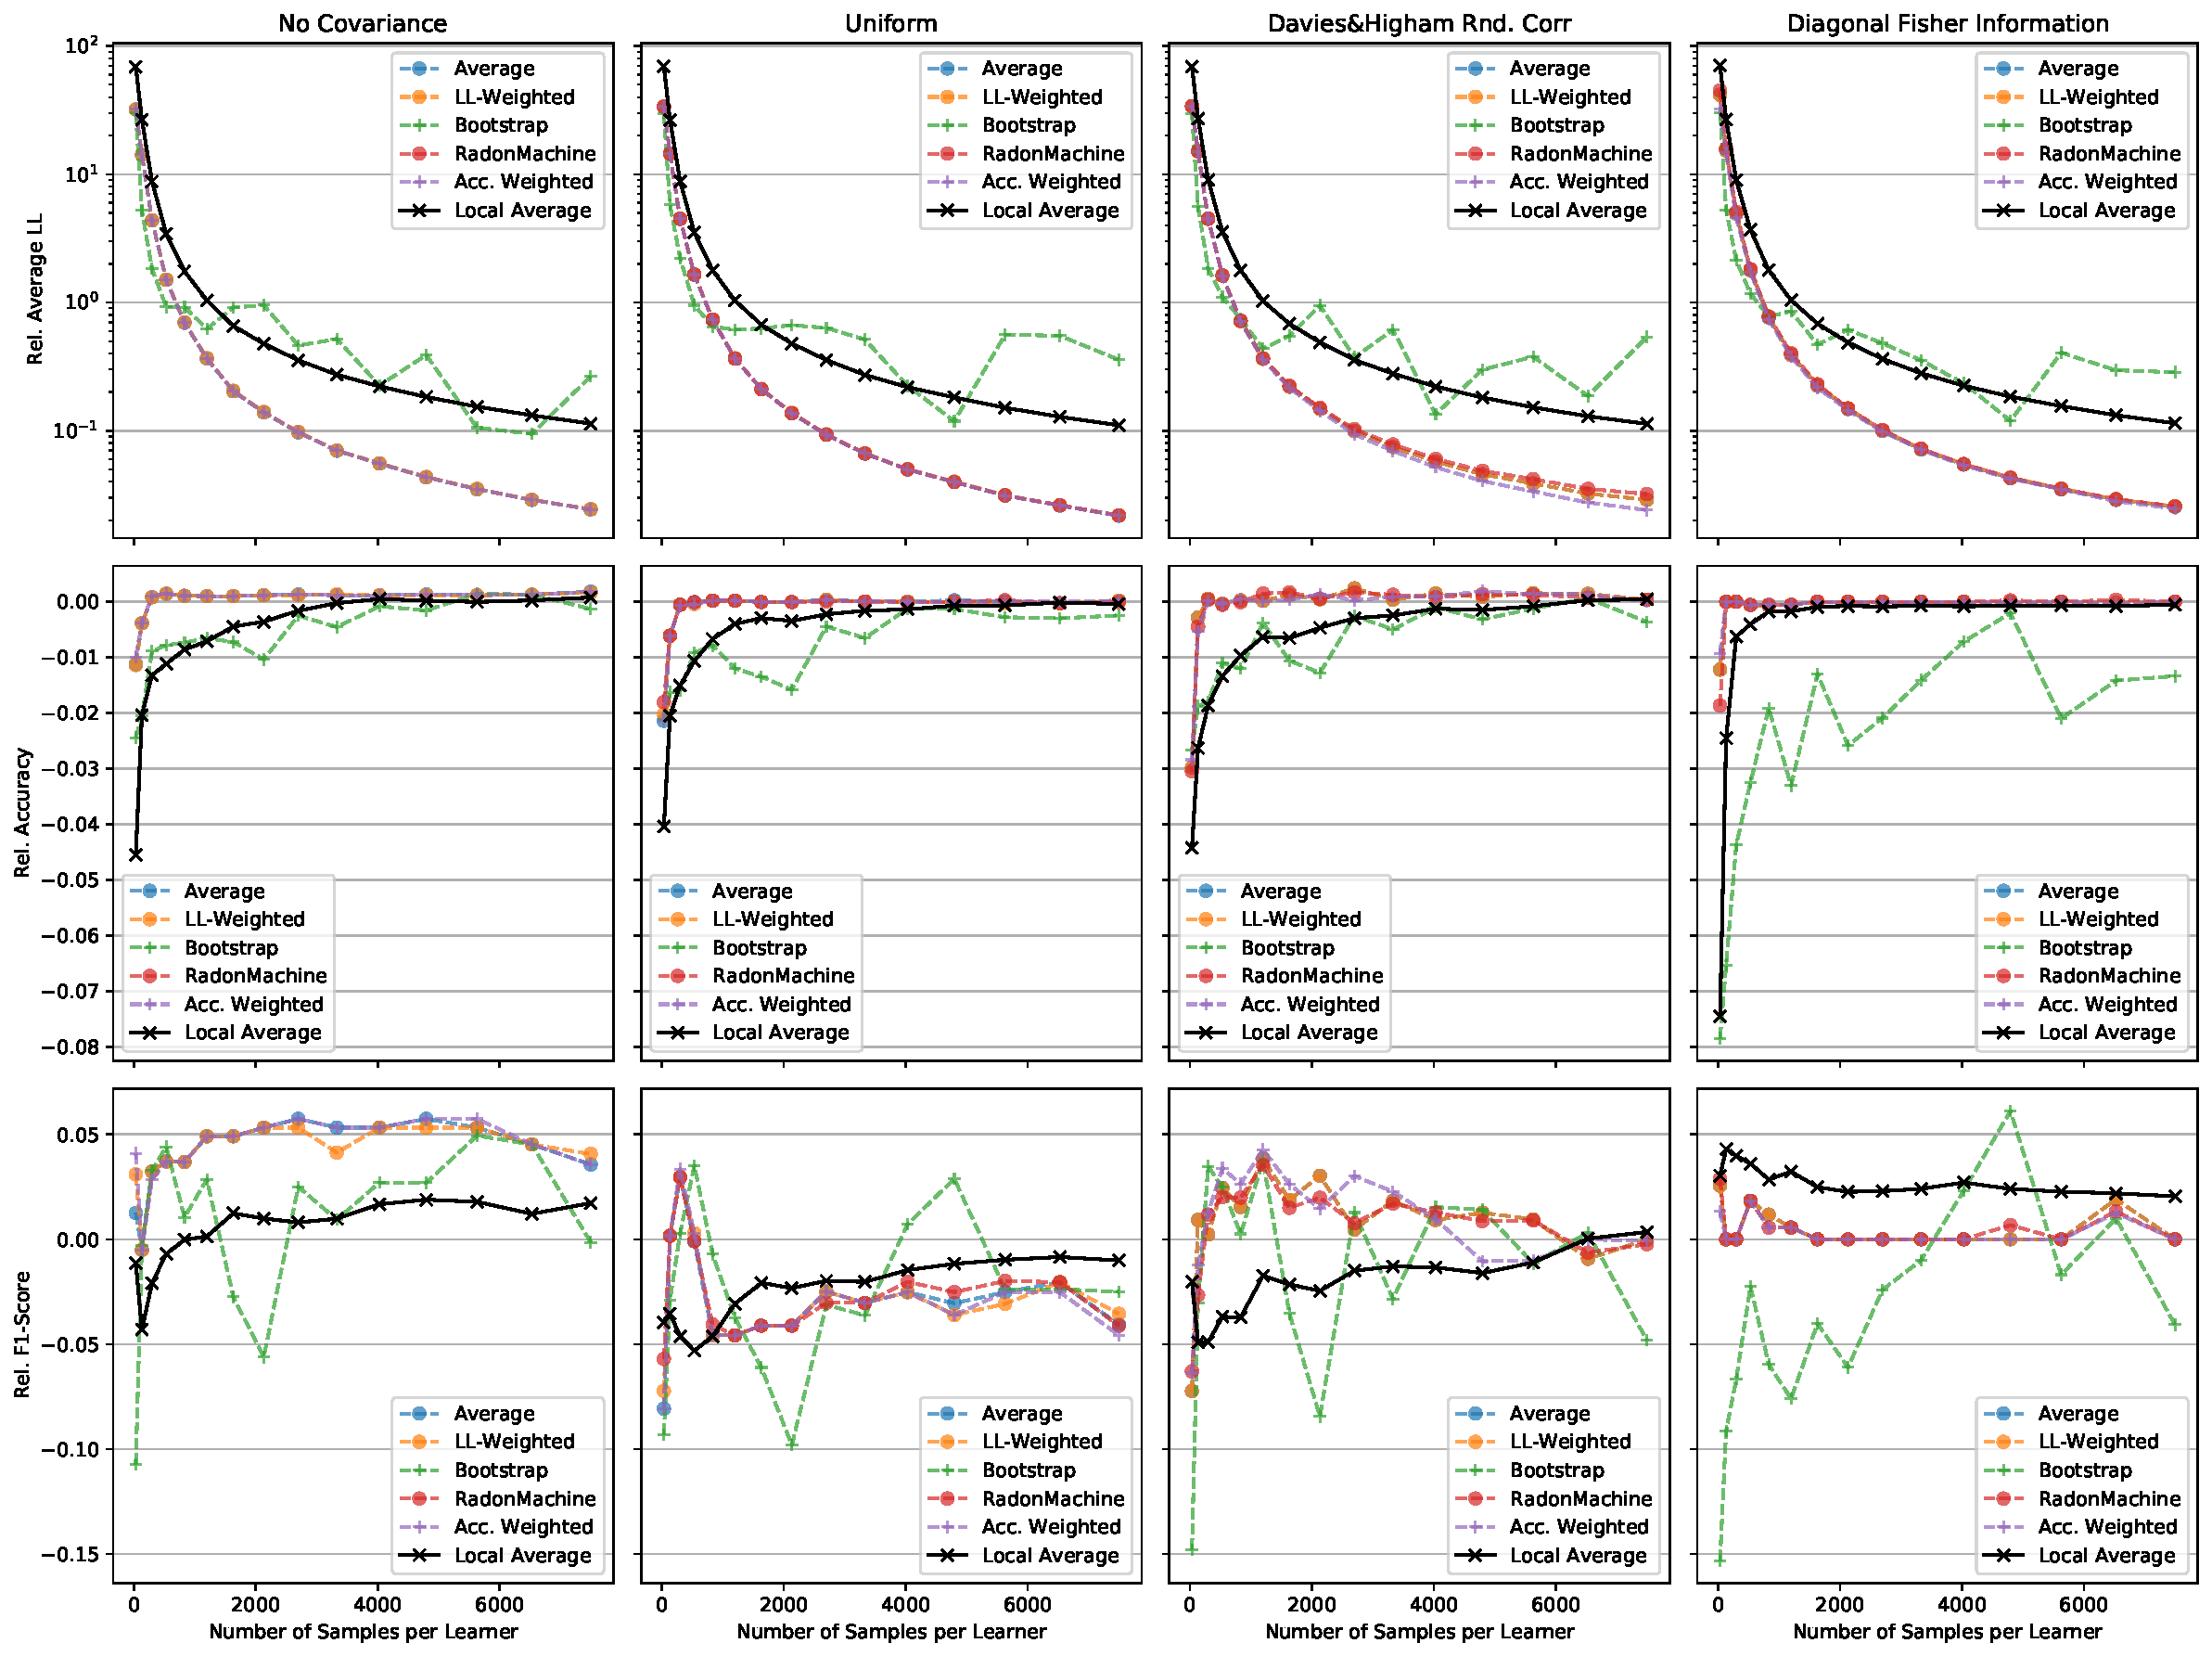
\includegraphics[height=\dimexpr \textheight - 4\baselineskip\relax]{kapitel/figures/susy_None_0.05_neg_relative.pdf}
        \caption[Susy without regularization and $\epsilon=0.05$]{Experimental results on the Susy data set for $k=10$ distributed learners. Each plot represents a combination of metric and covariance matrix used for sampling. Values on the x-Axis are the number of samples available on each learner. The top row shows the relative negative average log likelihood $\ell(\tilde{\vect{\theta}}; \mathcal{D}) - \ell(\hat{\vect{\theta}}; \mathcal{D})$ for each aggregate. Second and third row show accuracy and F1-score relative to the baseline on the test set.}
        \label{fig:analysis5}
    \end{figure}
    \end{landscape}
    \begin{landscape}
        \begin{figure}
            \centering
            \textbf{Susy, l2 regularization, Bound $\epsilon=0.1$}\par\medskip
            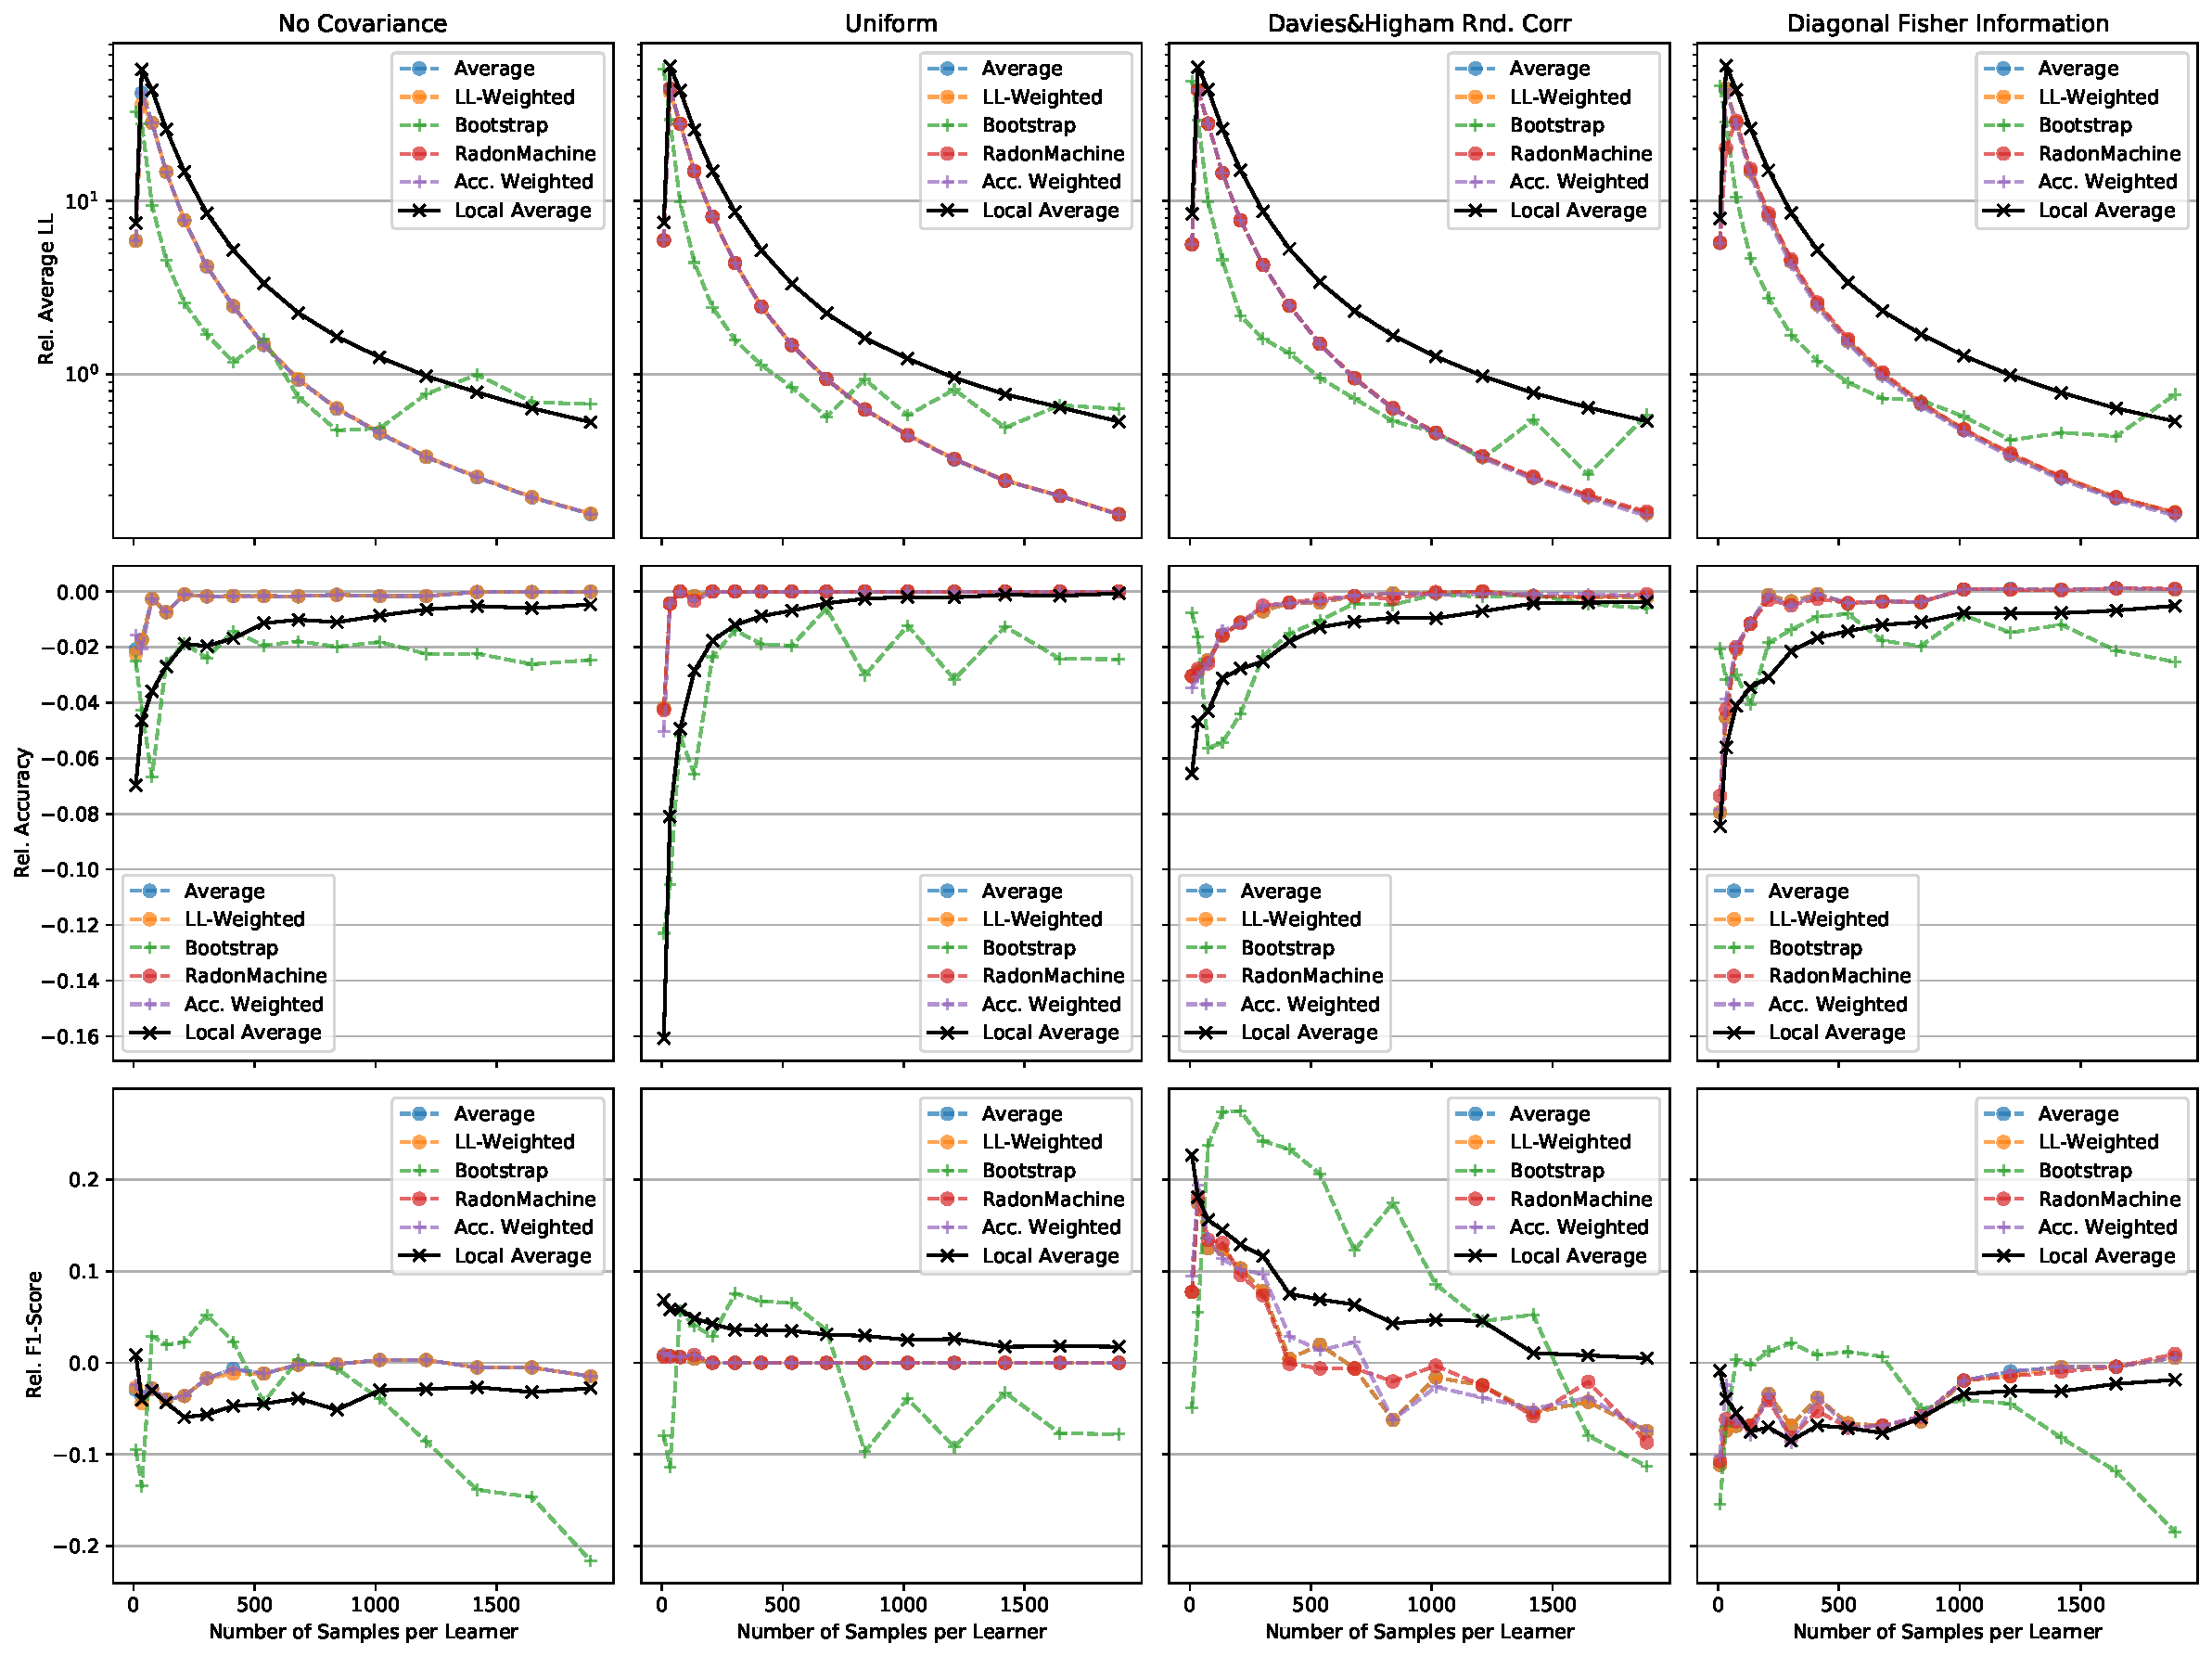
\includegraphics[height=\dimexpr \textheight - 4\baselineskip\relax]{kapitel/figures/susy_l2_0.1_neg_relative.pdf}
            \caption[Susy plots with l2 regularization and $\epsilon=0.1$]{Experimental results on the Susy data set for $k=10$ distributed learners. Each plot represents a combination of metric and covariance matrix used for sampling. Values on the x-Axis are the number of samples available on each learner. The top row shows the relative negative average log likelihood $\ell(\tilde{\vect{\theta}}; \mathcal{D}) - \ell(\hat{\vect{\theta}}; \mathcal{D})$ for each aggregate. Second and third row show accuracy and F1-score relative to the baseline on the test set.}
            \label{fig:analysis6}
        \end{figure}
    \end{landscape}

\begin{landscape}
    \begin{figure}
        \centering
        \textbf{Covertype, No regularization, Bound $\epsilon=0.1$}\par\medskip
        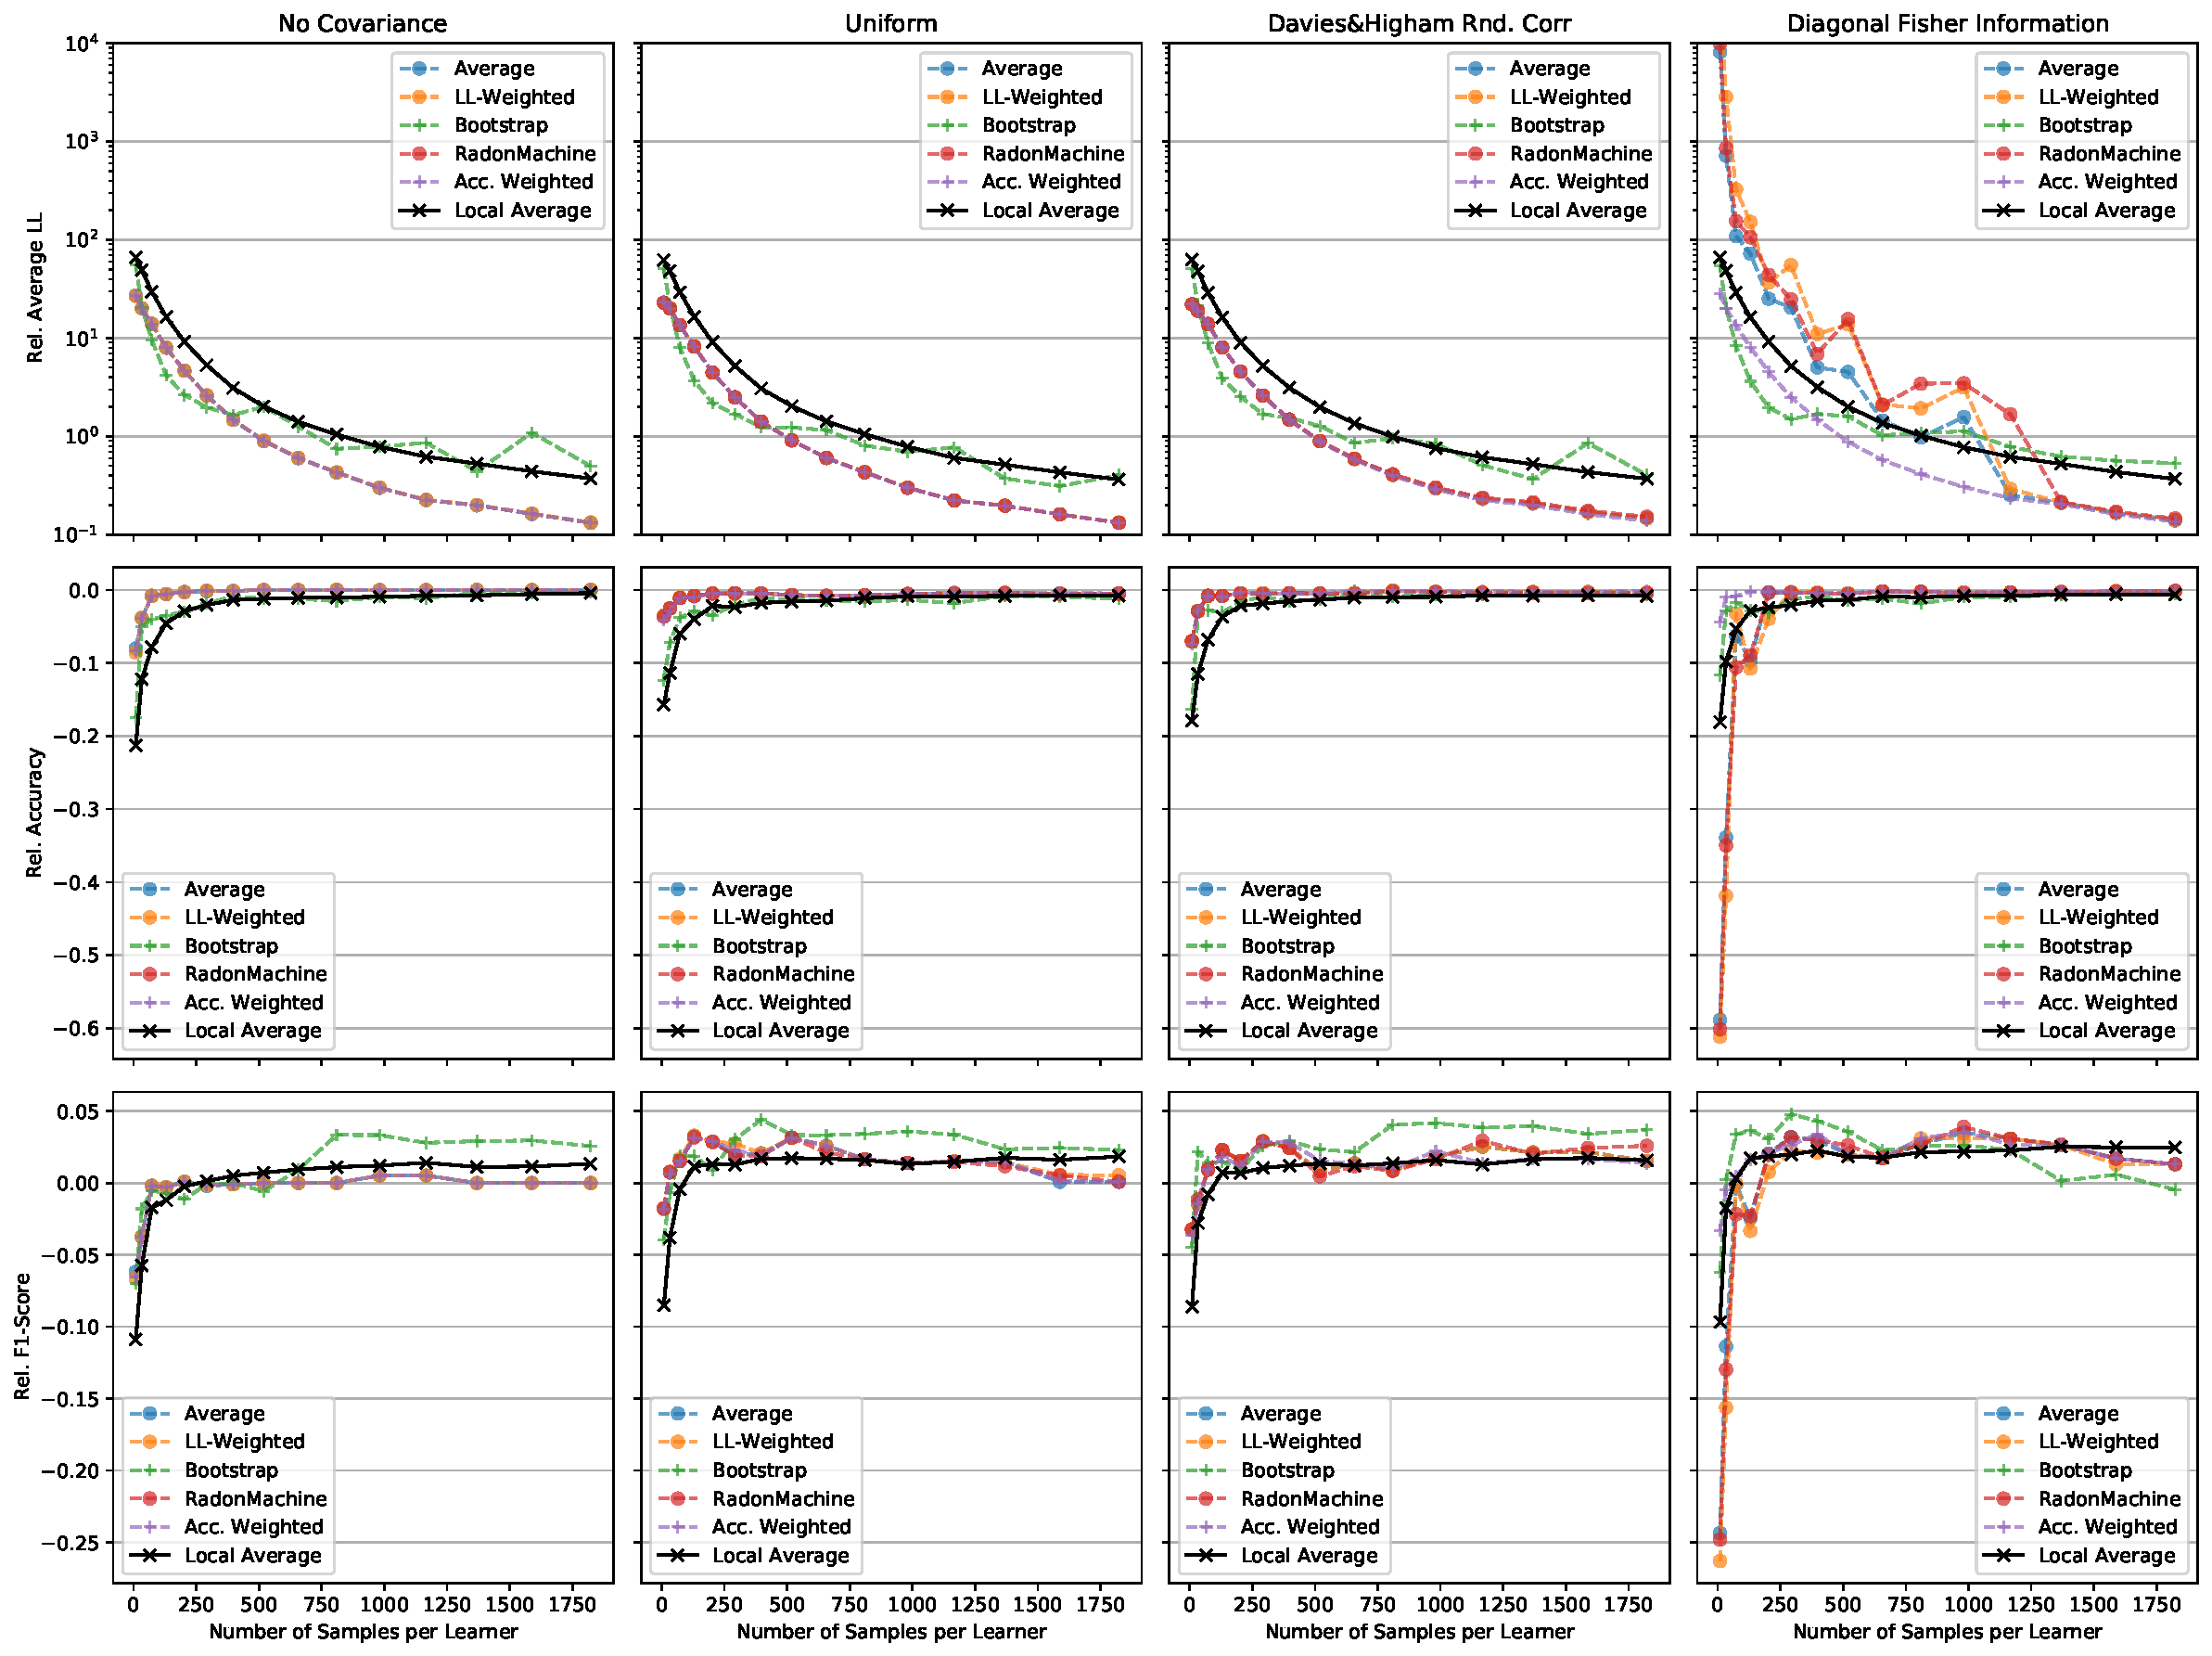
\includegraphics[height=\dimexpr \textheight - 4\baselineskip\relax]{kapitel/figures/covertype_None_0.1_neg_relative.pdf}
        \caption[Covertype plots without regularization and $\epsilon=0.1$]{Experimental results on the Covertype data set for $k=10$ distributed learners. Each plot represents a combination of metric and covariance matrix used for sampling. Values on the x-Axis are the number of samples available on each learner.The top row shows the relative negative average log likelihood $\ell(\tilde{\vect{\theta}}; \mathcal{D}) - \ell(\hat{\vect{\theta}}; \mathcal{D})$ for each aggregate. Second and third row show accuracy and F1-score relative to the baseline on the test set.}
        \label{fig:analysis7}
    \end{figure}
    \end{landscape}
    \begin{landscape}
    \begin{figure}
        \centering
        \textbf{Covertype, No regularization, Bound $\epsilon=0.05$}\par\medskip
        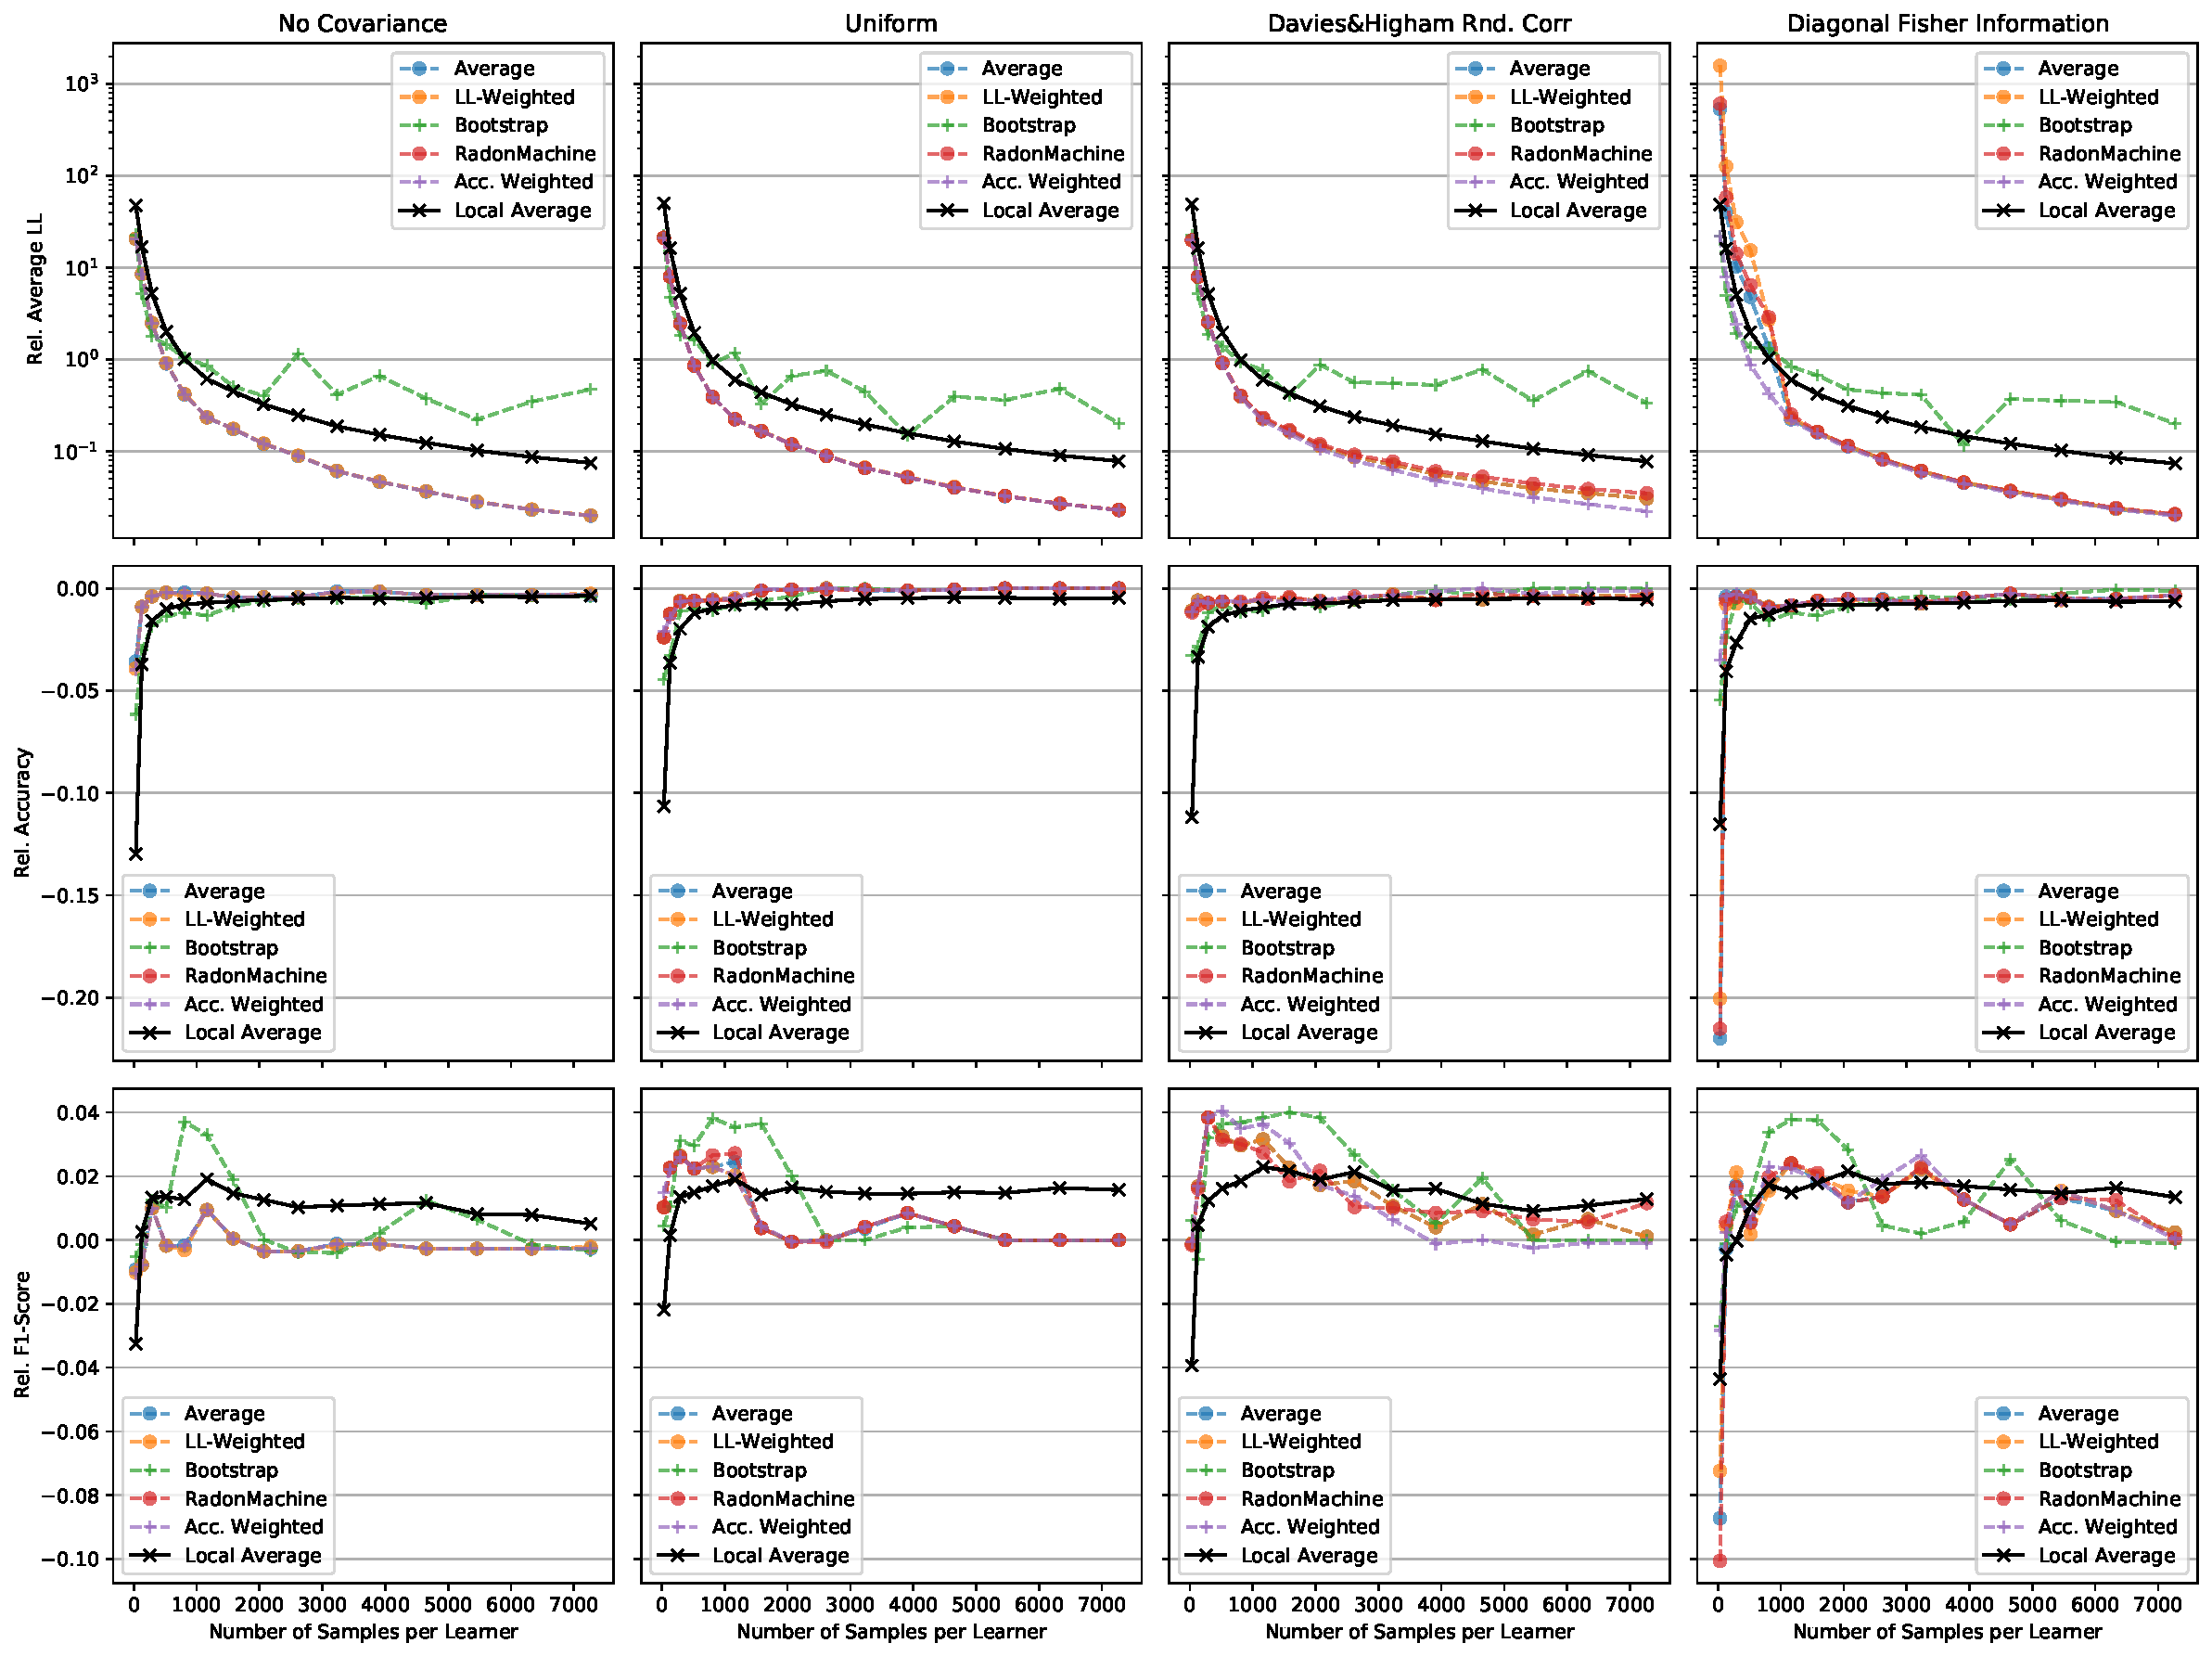
\includegraphics[height=\dimexpr \textheight - 4\baselineskip\relax]{kapitel/figures/covertype_None_0.05_neg_relative.pdf}
        \caption[Covertype without regularization and $\epsilon=0.05$]{Experimental results on the Covertype data set for $k=10$ distributed learners. Each plot represents a combination of metric and covariance matrix used for sampling. Values on the x-Axis are the number of samples available on each learner. The top row shows the relative negative average log likelihood $\ell(\tilde{\vect{\theta}}; \mathcal{D}) - \ell(\hat{\vect{\theta}}; \mathcal{D})$ for each aggregate. Second and third row show accuracy and F1-score relative to the baseline on the test set.}
        \label{fig:analysis8}
    \end{figure}
    \end{landscape}
    \begin{landscape}
        \begin{figure}
            \centering
            \textbf{Covertype, l2 regularization, Bound $\epsilon=0.1$}\par\medskip
            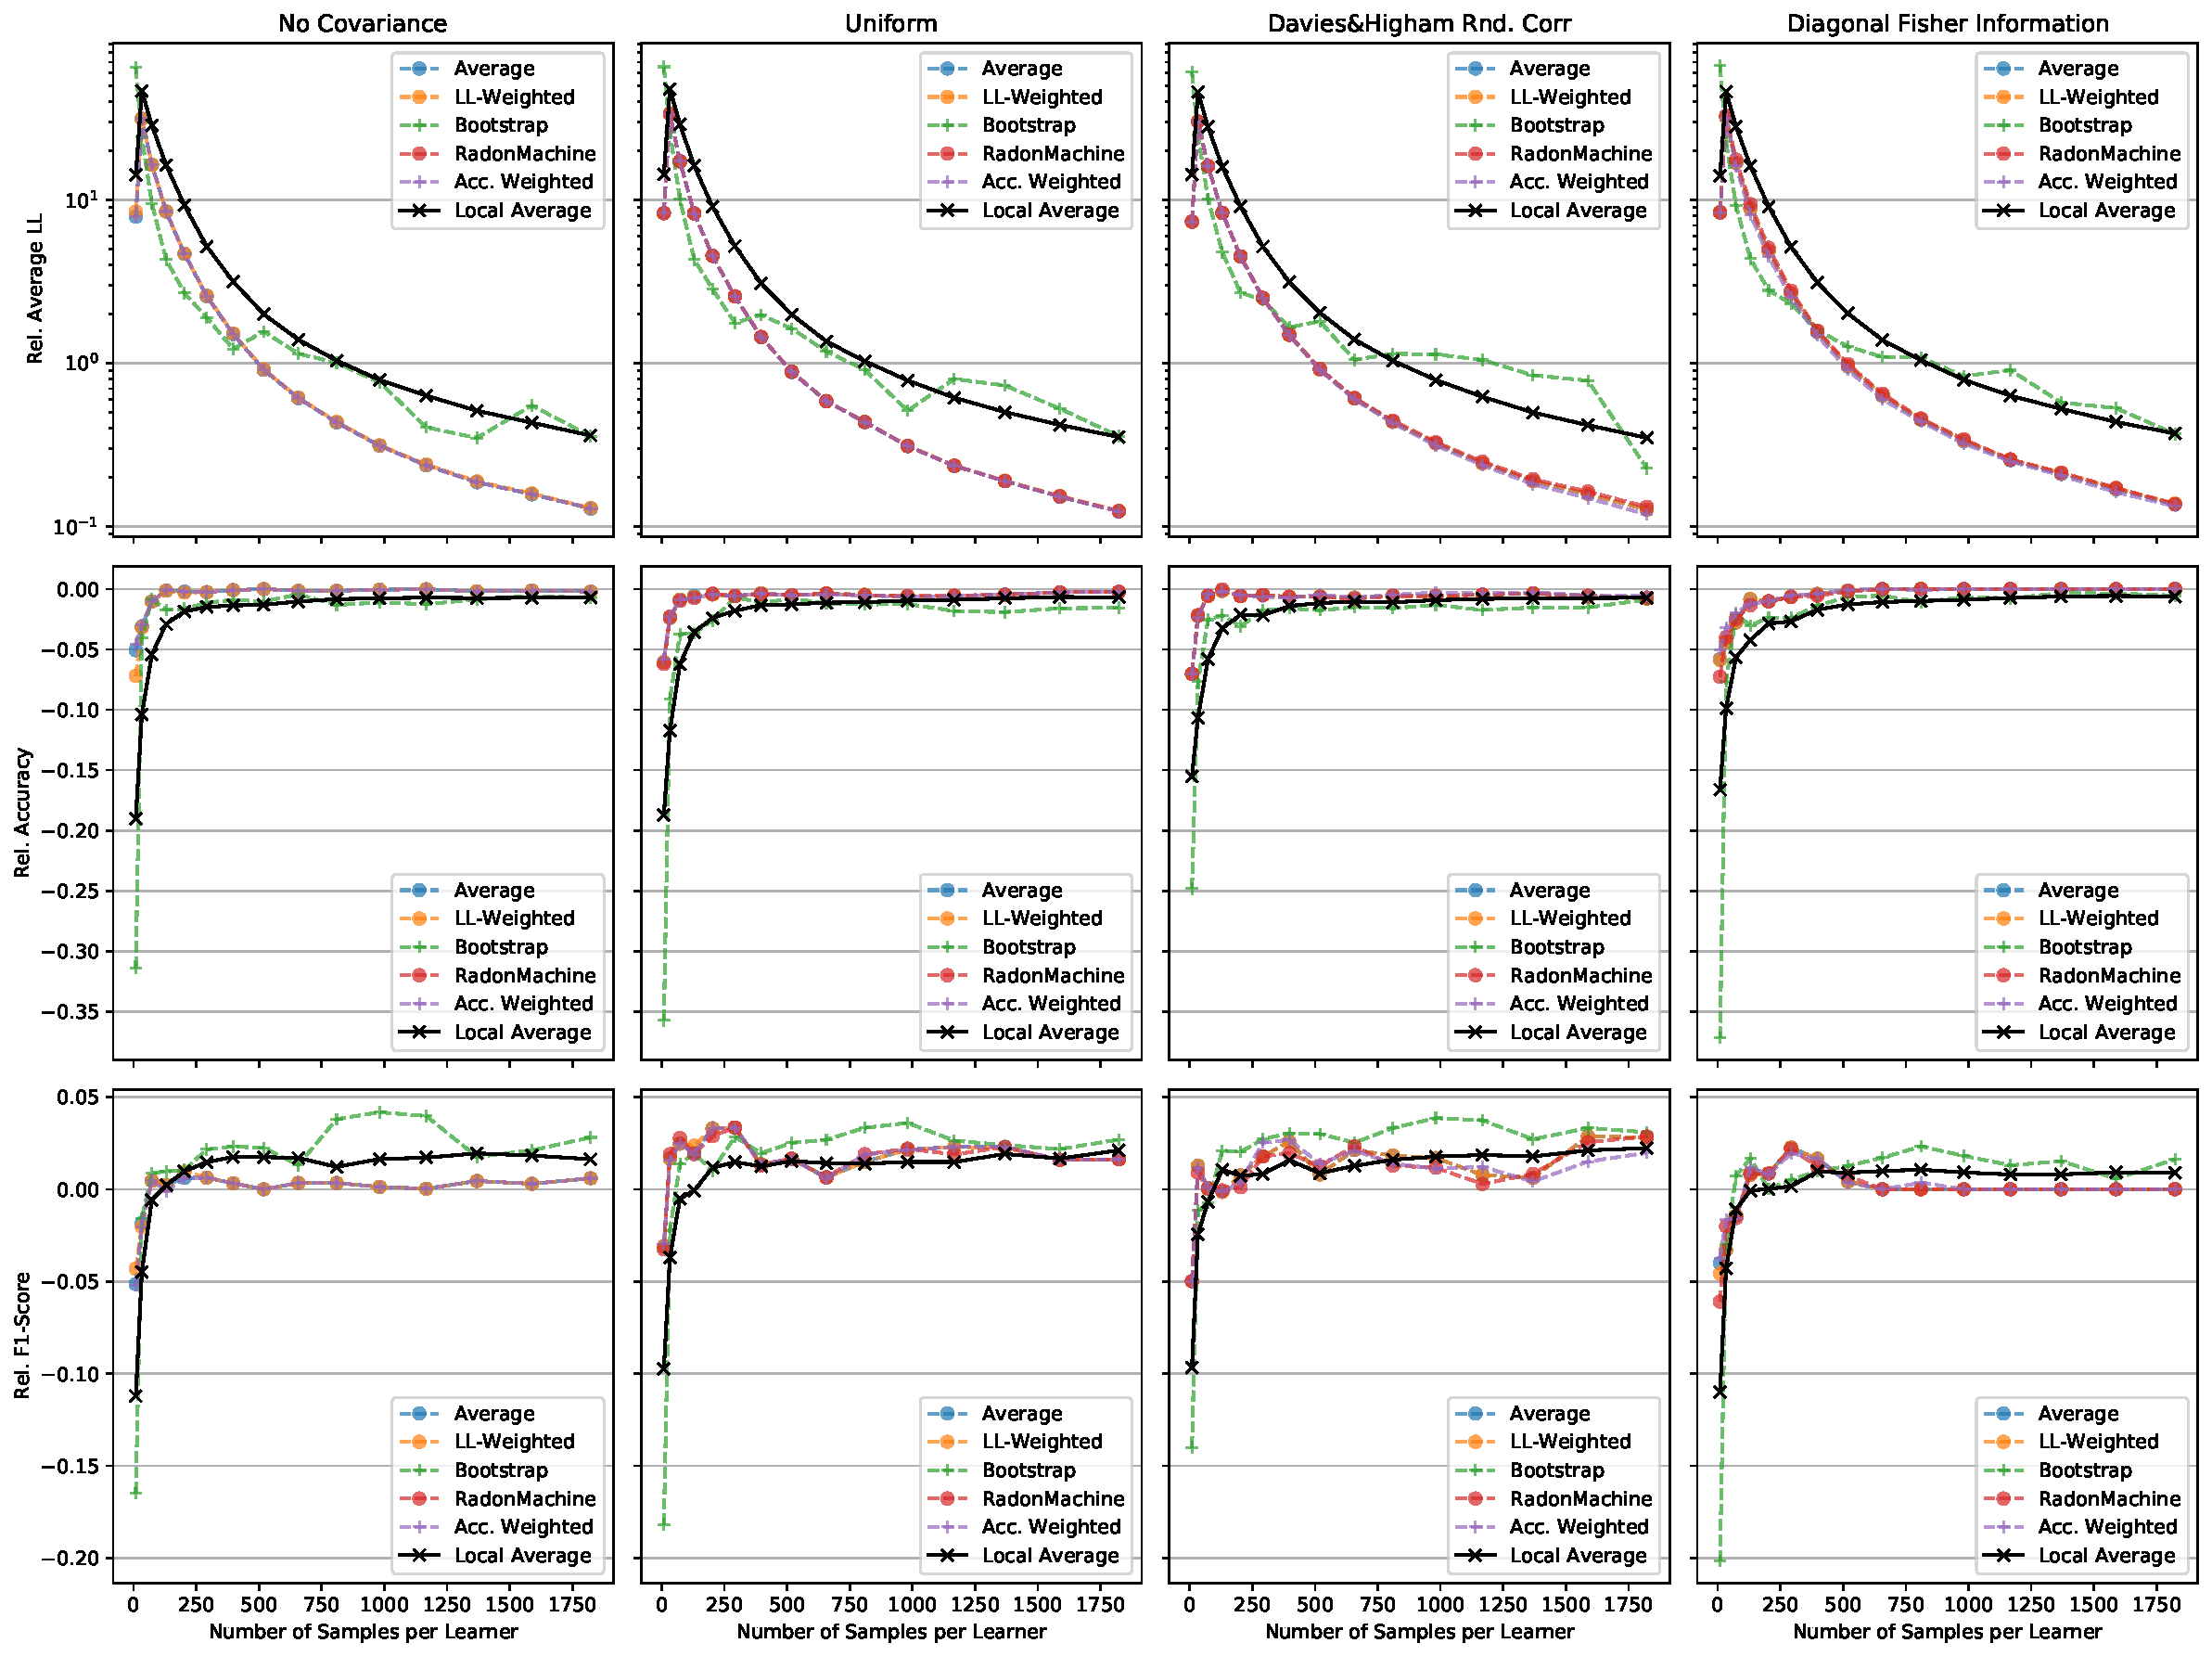
\includegraphics[height=\dimexpr \textheight - 4\baselineskip\relax]{kapitel/figures/covertype_l2_0.1_neg_relative.pdf}
            \caption[Covertype plots with l2 regularization and $\epsilon=0.1$]{Experimental results on the Covertype data set for $k=10$ distributed learners. Each plot represents a combination of metric and covariance matrix used for sampling. Values on the x-Axis are the number of samples available on each learner. The top row shows the relative negative average log likelihood $\ell(\tilde{\vect{\theta}}; \mathcal{D}) - \ell(\hat{\vect{\theta}}; \mathcal{D})$ for each aggregate. Second and third row show accuracy and F1-score relative to the baseline on the test set.}
            \label{fig:analysis9}
        \end{figure}
    \end{landscape}

\begin{landscape}
    \begin{figure}
        \centering
        \textbf{Dota2, No regularization, Bound $\epsilon=0.1$}\par\medskip
        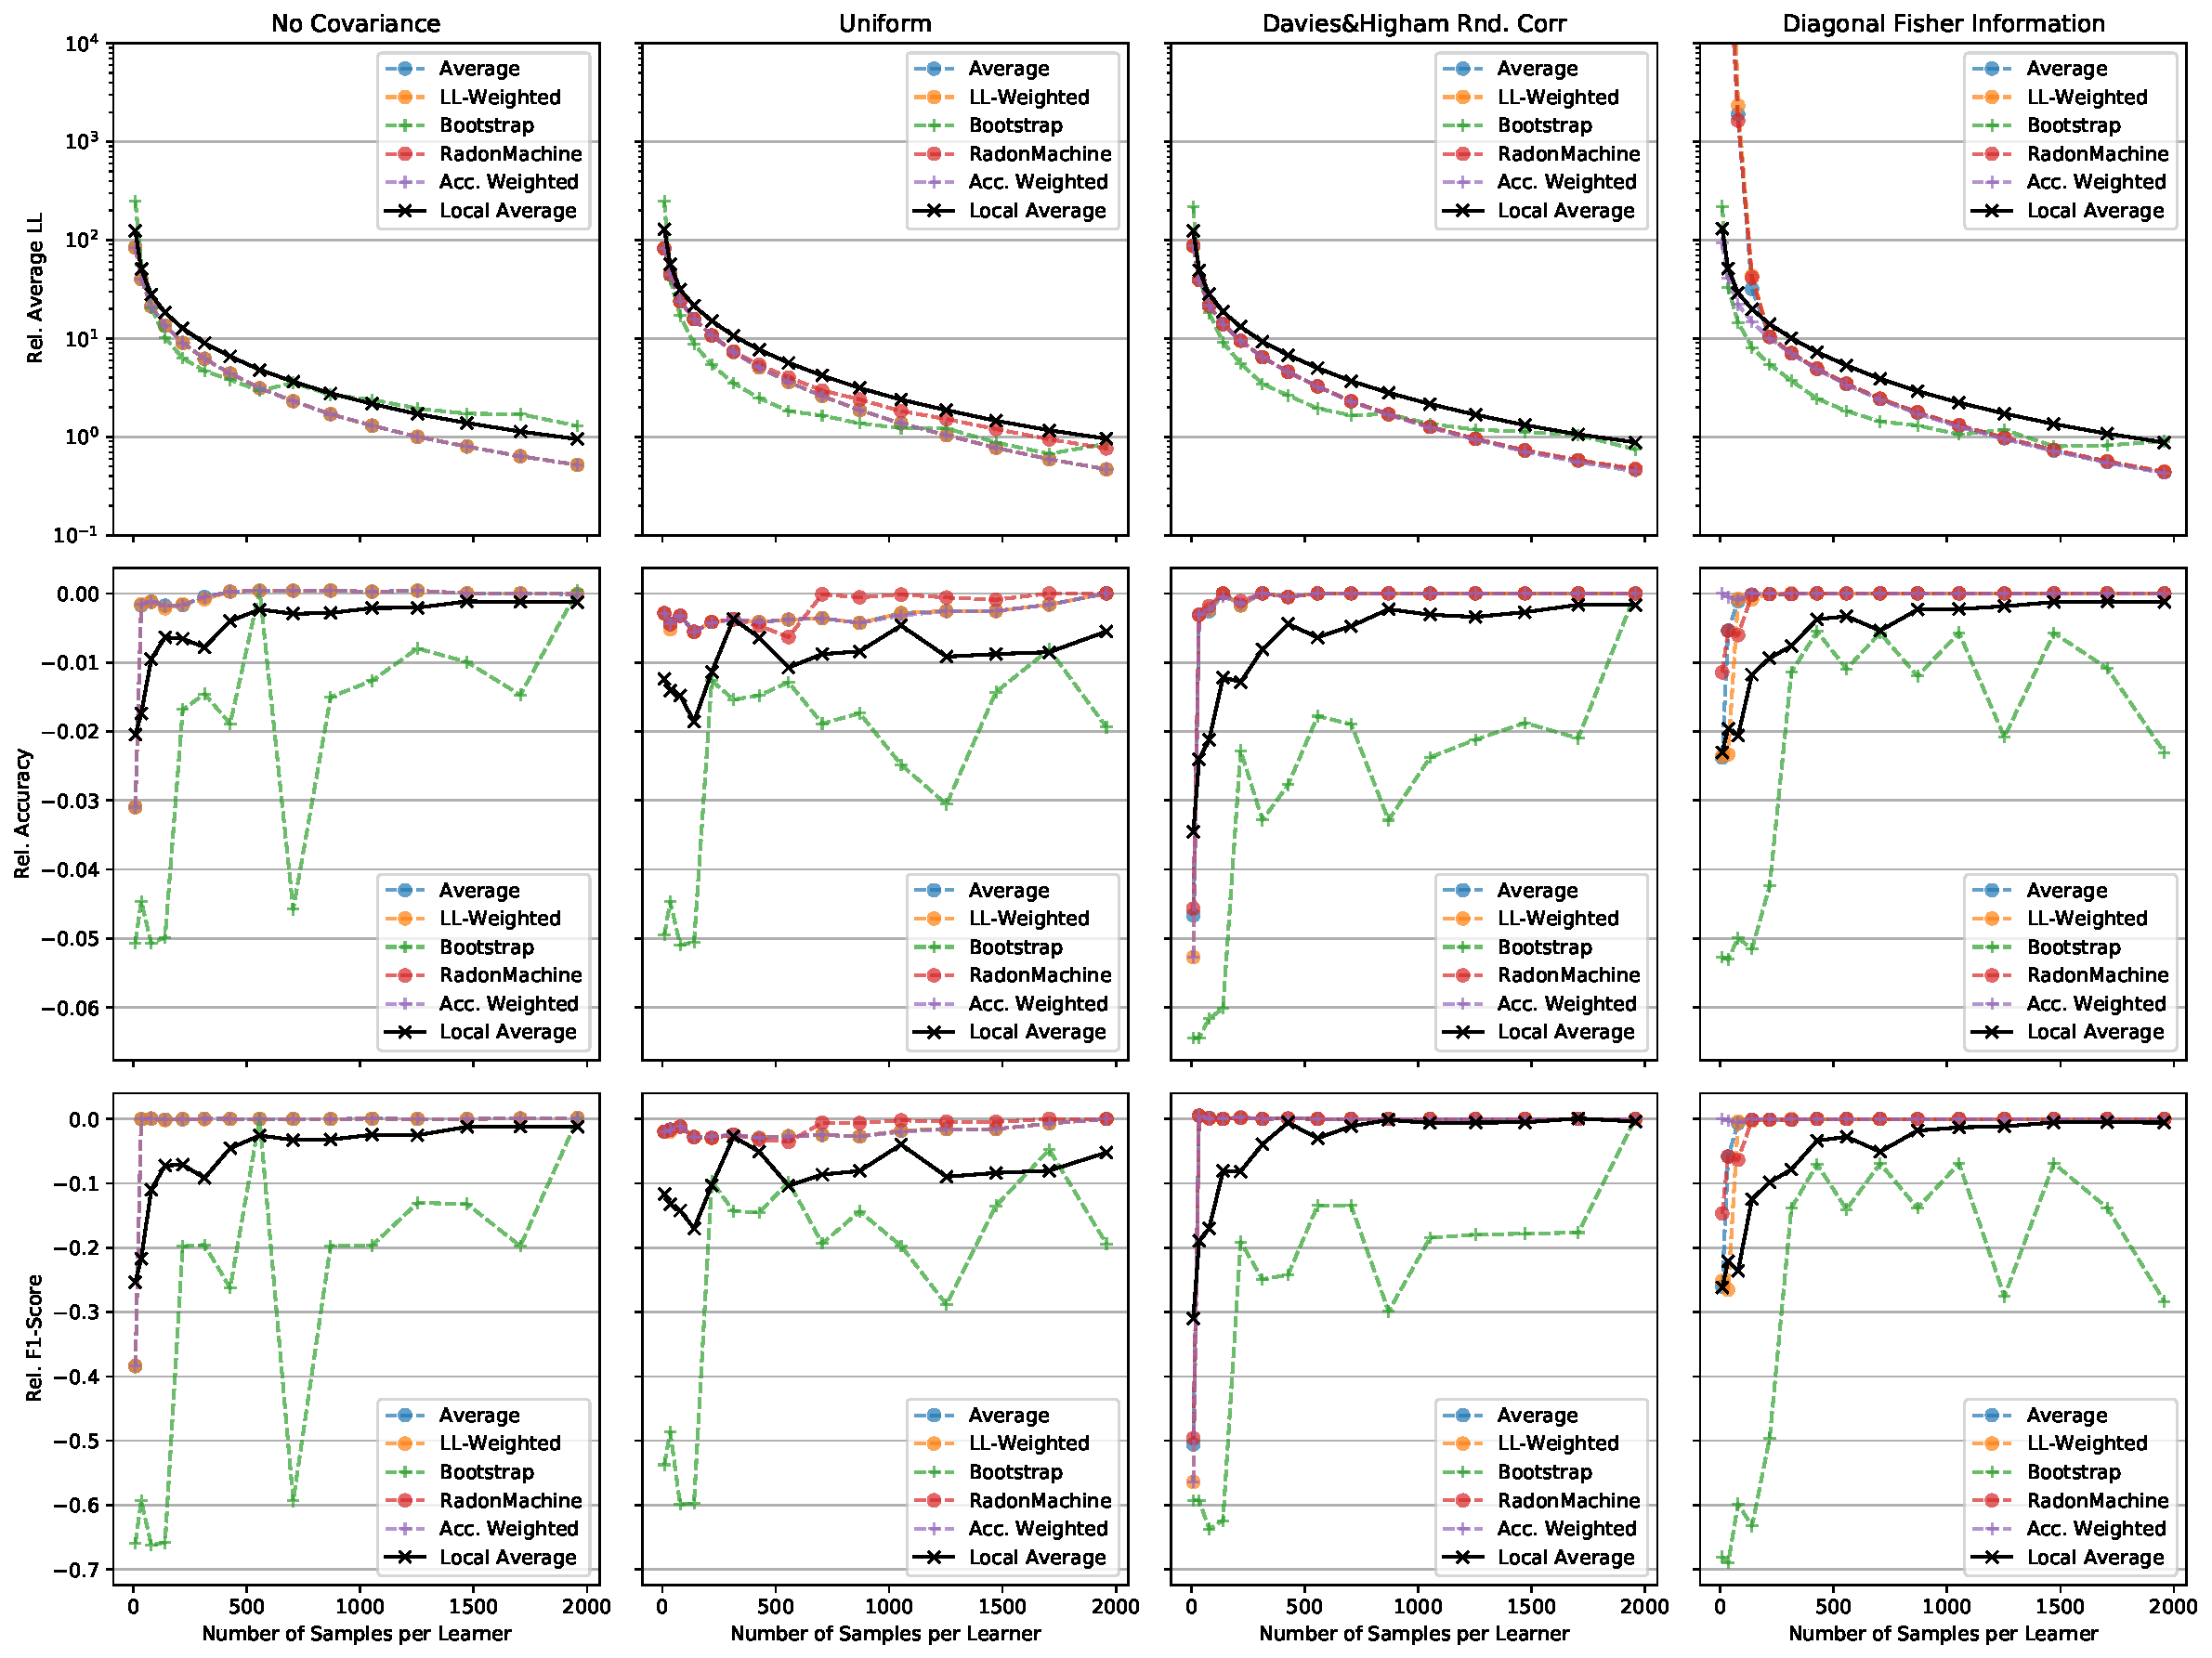
\includegraphics[height=\dimexpr \textheight - 4\baselineskip\relax]{kapitel/figures/dota2_None_0.1_neg_relative.pdf}
        \caption[Dota2 plots without regularization and $\epsilon=0.1$]{Experimental results on the Dota2 data set for $k=10$ distributed learners. Each plot represents a combination of metric and covariance matrix used for sampling. Values on the x-Axis are the number of samples available on each learner.The top row shows the relative negative average log likelihood $\ell(\tilde{\vect{\theta}}; \mathcal{D}) - \ell(\hat{\vect{\theta}}; \mathcal{D})$ for each aggregate. Second and third row show accuracy and F1-score relative to the baseline on the test set.}
        \label{fig:analysis10}
    \end{figure}
    \end{landscape}
    \begin{landscape}
    \begin{figure}
        \centering
        \textbf{Dota2, No regularization, Bound $\epsilon=0.05$}\par\medskip
        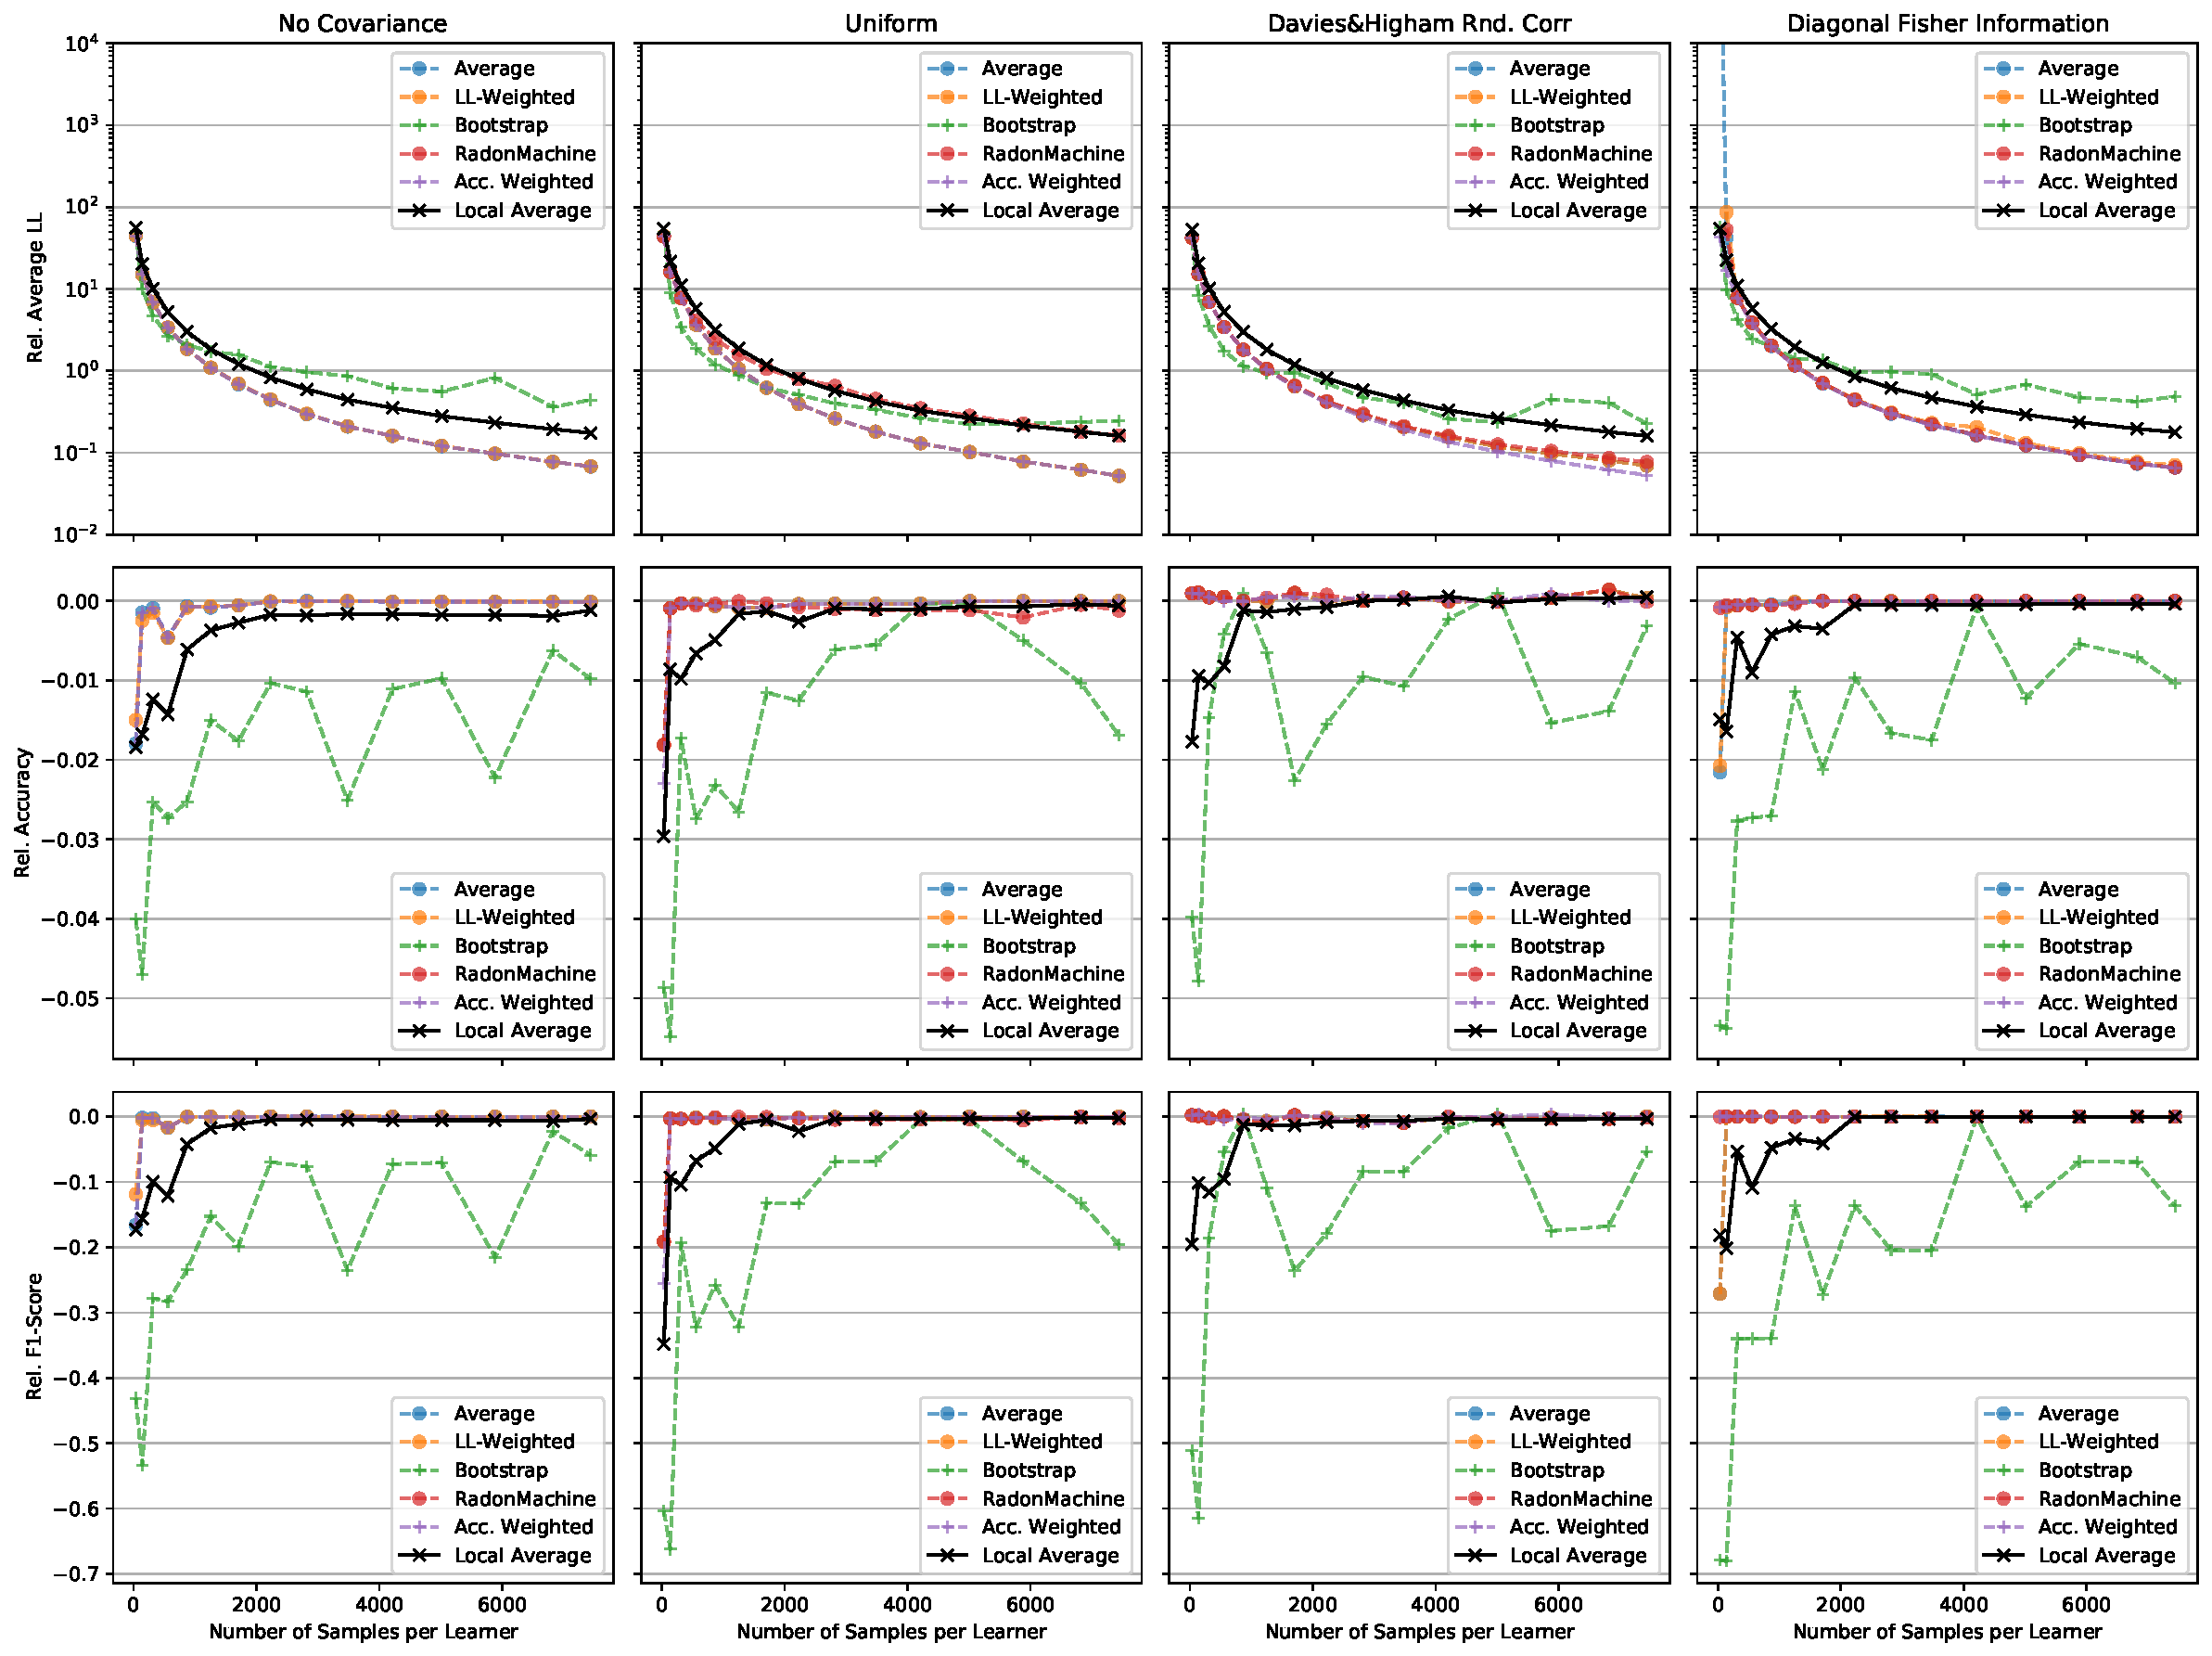
\includegraphics[height=\dimexpr \textheight - 4\baselineskip\relax]{kapitel/figures/dota2_None_0.05_neg_relative.pdf}
        \caption[Dota2 plots without regularization and $\epsilon=0.05$]{Experimental results on the Dota2 data set for $k=10$ distributed learners. Each plot represents a combination of metric and covariance matrix used for sampling. Values on the x-Axis are the number of samples available on each learner.The top row shows the relative negative average log likelihood $\ell(\tilde{\vect{\theta}}; \mathcal{D}) - \ell(\hat{\vect{\theta}}; \mathcal{D})$ for each aggregate. Second and third row show accuracy and F1-score relative to the baseline on the test set.}
        \label{fig:analysis11}
    \end{figure}
    \end{landscape}
    \begin{landscape}
        \begin{figure}
            \centering
            \textbf{Dota2, l2 regularization, Bound $\epsilon=0.1$}\par\medskip
            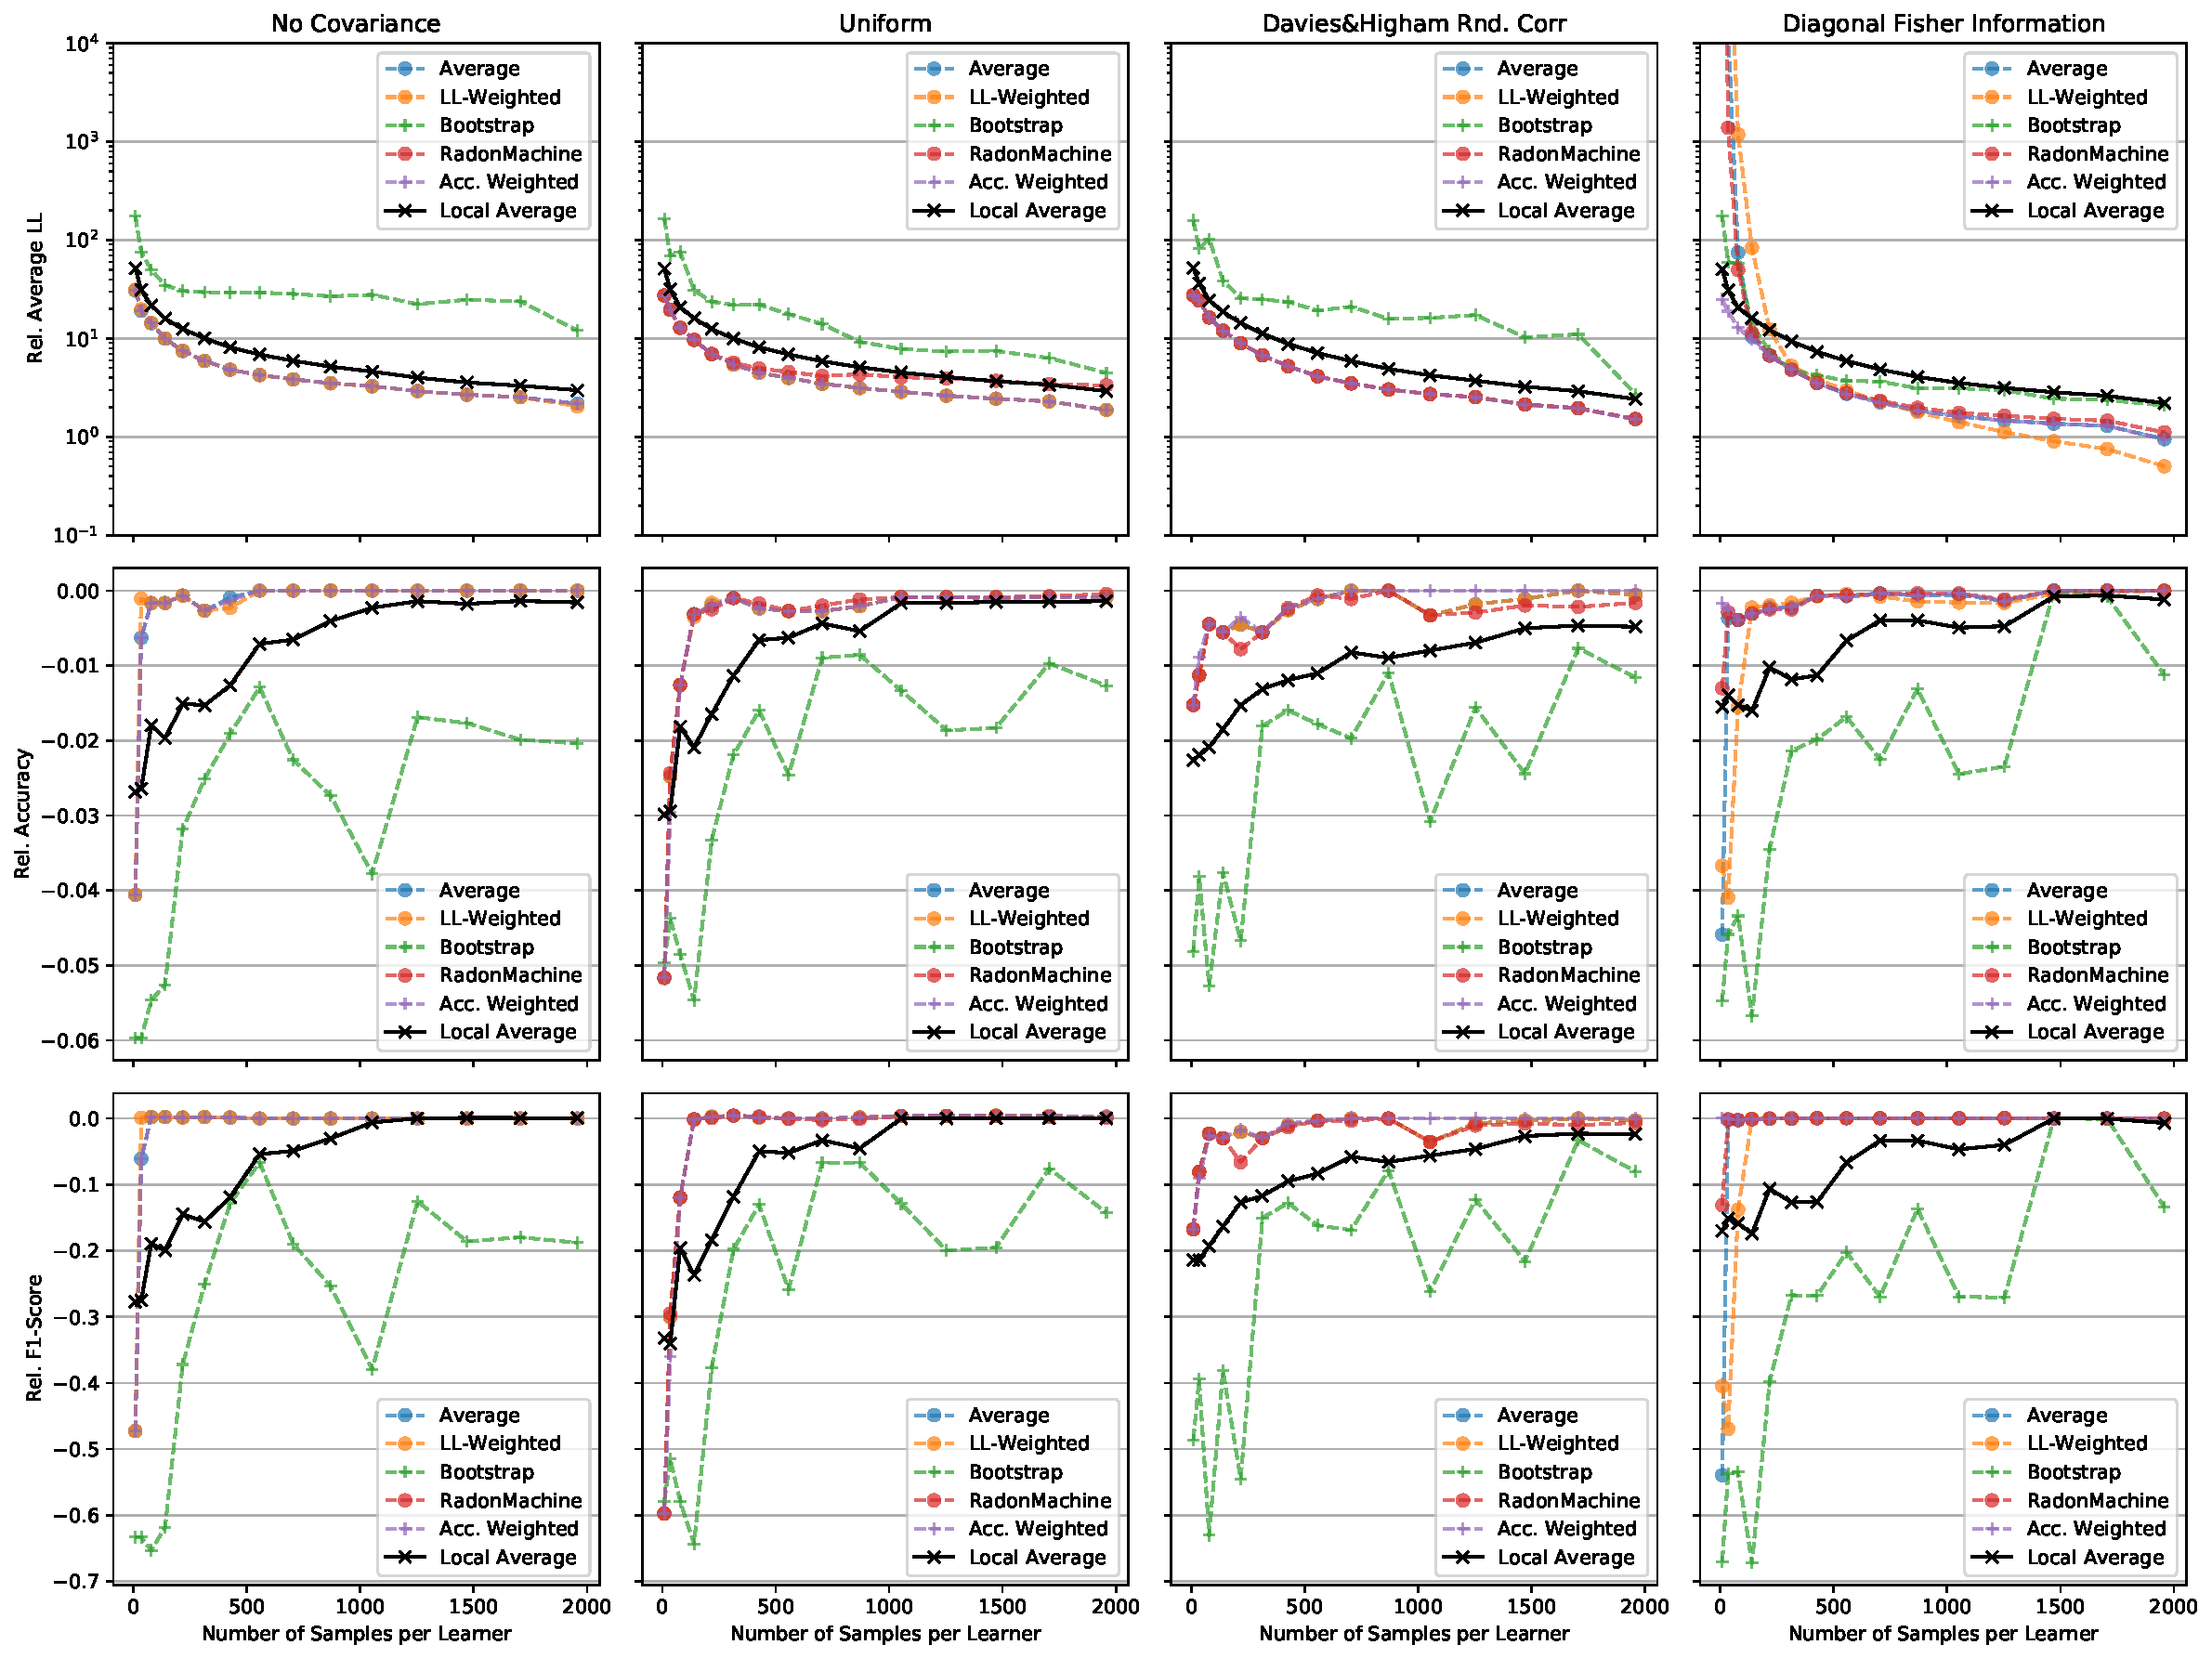
\includegraphics[height=\dimexpr \textheight - 4\baselineskip\relax]{kapitel/figures/dota2_l2_0.1_neg_relative.pdf}
            \caption[Dota2 plots with l2 regularization and $\epsilon=0.1$]{Experimental results on the Dota2 data set for $k=10$ distributed learners. Each plot represents a combination of metric and covariance matrix used for sampling. Values on the x-Axis are the number of samples available on each learner. The top row shows the relative negative average log likelihood $\ell(\tilde{\vect{\theta}}; \mathcal{D}) - \ell(\hat{\vect{\theta}}; \mathcal{D})$ for each aggregate. Second and third row show accuracy and F1-score relative to the baseline on the test set.}
            \label{fig:analysis12}
        \end{figure}
    \end{landscape}

\section{Independence Structures}
\label{sec:apdx:struc}

\begin{figure}[!htb]
\center
\centering
\textbf{Independence Graph for Susy generated by the Chow-Liu algorithm}\par\medskip
\begin{tikzpicture}
\clip (0,0) rectangle (17.0,15.0);
\Vertex[x=5.611,y=13.063,size=0.5,color=blue,opacity=0.7]{0}
\Vertex[x=7.389,y=12.774,size=0.5,color=tuorange,opacity=0.7]{2}
\Vertex[x=9.526,y=11.806,size=0.5,color=tugreen,opacity=0.7]{1}
\Vertex[x=11.448,y=10.109,size=0.5,color=tuorange,opacity=0.7]{11}
\Vertex[x=6.818,y=14.000,size=0.5,color=tugreen,opacity=0.7]{5}
\Vertex[x=13.820,y=3.181,size=0.5,color=tugreen,opacity=0.7]{3}
\Vertex[x=12.432,y=1.605,size=0.5,color=tuorange,opacity=0.7]{6}
\Vertex[x=13.892,y=5.464,size=0.5,color=tuorange,opacity=0.7]{8}
\Vertex[x=12.896,y=7.850,size=0.5,color=tugreen,opacity=0.7]{4}
\Vertex[x=9.531,y=5.061,size=0.5,color=tugreen,opacity=0.7]{7}
\Vertex[x=6.976,y=4.562,size=0.5,color=tuorange,opacity=0.7]{9}
\Vertex[x=11.070,y=4.835,size=0.5,color=tuorange,opacity=0.7]{10}
\Vertex[x=10.298,y=7.228,size=0.5,color=tuorange,opacity=0.7]{12}
\Vertex[x=8.875,y=2.780,size=0.5,color=tuorange,opacity=0.7]{13}
\Vertex[x=11.669,y=6.020,size=0.5,color=tuorange,opacity=0.7]{17}
\Vertex[x=4.788,y=3.995,size=0.5,color=tugreen,opacity=0.7]{16}
\Vertex[x=11.329,y=8.920,size=0.5,color=tugreen,opacity=0.7]{15}
\Vertex[x=8.393,y=1.000,size=0.5,color=tugreen,opacity=0.7]{18}
\Vertex[x=3.108,y=3.487,size=0.5,color=tuorange,opacity=0.7]{14}
\Edge[,lw=0.1,color=black](0)(2)
\Edge[,lw=0.1,color=black](2)(1)
\Edge[,lw=0.1,color=black](2)(5)
\Edge[,lw=0.1,color=black](1)(11)
\Edge[,lw=0.1,color=black](11)(4)
\Edge[,lw=0.1,color=black](11)(15)
\Edge[,lw=0.1,color=black](3)(6)
\Edge[,lw=0.1,color=black](3)(8)
\Edge[,lw=0.1,color=black](8)(4)
\Edge[,lw=0.1,color=black](7)(9)
\Edge[,lw=0.1,color=black](7)(10)
\Edge[,lw=0.1,color=black](7)(12)
\Edge[,lw=0.1,color=black](7)(13)
\Edge[,lw=0.1,color=black](7)(17)
\Edge[,lw=0.1,color=black](9)(16)
\Edge[,lw=0.1,color=black](12)(15)
\Edge[,lw=0.1,color=black](13)(18)
\Edge[,lw=0.1,color=black](16)(14)
\end{tikzpicture}
\caption[Approximated independence structure of the Susy data set]{Tree estimated with the Chow-Liu algorithm. Neighboring nodes are displayed with alternating colors generated from a 2-Coloring algorithm to improve visibility. The root, which is the random variable for the labels, is shown in blue.}
\label{fig:susy_ind}
\end{figure}
\begin{figure}[!htb]
    \center
    \textbf{Independence Graph for Covertype generated by the Chow-Liu algorithm}\par\medskip
    \resizebox{\linewidth}{!}{%
    \begin{tikzpicture}
        \clip (0,0) rectangle (17.0,15.0);
        \Vertex[x=12.637,y=6.951,size=0.5,color=tuorange,opacity=0.7]{0}
        \Vertex[x=13.224,y=8.670,size=0.5,color=tugreen,opacity=0.7]{3}
        \Vertex[x=14.502,y=6.725,size=0.5,color=tugreen,opacity=0.7]{5}
        \Vertex[x=12.634,y=8.090,size=0.5,color=tugreen,opacity=0.7]{9}
        \Vertex[x=10.487,y=5.452,size=0.5,color=blue,opacity=0.7]{54}
        \Vertex[x=8.715,y=11.565,size=0.5,color=tugreen,opacity=0.7]{1}
        \Vertex[x=7.132,y=12.694,size=0.5,color=tuorange,opacity=0.7]{6}
        \Vertex[x=10.448,y=11.497,size=0.5,color=tuorange,opacity=0.7]{7}
        \Vertex[x=8.610,y=10.130,size=0.5,color=tuorange,opacity=0.7]{8}
        \Vertex[x=12.001,y=11.238,size=0.5,color=tugreen,opacity=0.7]{2}
        \Vertex[x=13.029,y=10.213,size=0.5,color=tuorange,opacity=0.7]{4}
        \Vertex[x=15.279,y=6.087,size=0.5,color=tuorange,opacity=0.7]{14}
        \Vertex[x=15.747,y=6.864,size=0.5,color=tuorange,opacity=0.7]{15}
        \Vertex[x=5.924,y=13.037,size=0.5,color=tugreen,opacity=0.7]{10}
        \Vertex[x=7.538,y=13.901,size=0.5,color=tugreen,opacity=0.7]{11}
        \Vertex[x=6.827,y=14.000,size=0.5,color=tugreen,opacity=0.7]{12}
        \Vertex[x=5.999,y=11.852,size=0.5,color=tugreen,opacity=0.7]{13}
        \Vertex[x=6.440,y=12.705,size=0.5,color=tugreen,opacity=0.7]{16}
        \Vertex[x=5.108,y=11.775,size=0.5,color=tuorange,opacity=0.7]{43}
        \Vertex[x=10.085,y=7.026,size=0.5,color=tuorange,opacity=0.7]{17}
        \Vertex[x=2.368,y=11.619,size=0.5,color=tuorange,opacity=0.7]{18}
        \Vertex[x=1.253,y=12.024,size=0.5,color=tugreen,opacity=0.7]{19}
        \Vertex[x=1.757,y=12.689,size=0.5,color=tugreen,opacity=0.7]{20}
        \Vertex[x=3.959,y=10.329,size=0.5,color=tugreen,opacity=0.7]{27}
        \Vertex[x=10.642,y=6.917,size=0.5,color=tuorange,opacity=0.7]{21}
        \Vertex[x=5.790,y=4.399,size=0.5,color=tuorange,opacity=0.7]{22}
        \Vertex[x=6.961,y=3.509,size=0.5,color=tugreen,opacity=0.7]{32}
        \Vertex[x=8.659,y=2.745,size=0.5,color=tuorange,opacity=0.7]{23}
        \Vertex[x=6.917,y=5.374,size=0.5,color=tugreen,opacity=0.7]{33}
        \Vertex[x=8.551,y=1.000,size=0.5,color=tugreen,opacity=0.7]{34}
        \Vertex[x=9.886,y=3.161,size=0.5,color=tugreen,opacity=0.7]{35}
        \Vertex[x=7.809,y=2.199,size=0.5,color=tugreen,opacity=0.7]{36}
        \Vertex[x=7.463,y=2.745,size=0.5,color=tugreen,opacity=0.7]{37}
        \Vertex[x=9.674,y=1.333,size=0.5,color=tugreen,opacity=0.7]{38}
        \Vertex[x=10.054,y=1.846,size=0.5,color=tugreen,opacity=0.7]{39}
        \Vertex[x=9.150,y=1.055,size=0.5,color=tugreen,opacity=0.7]{40}
        \Vertex[x=9.626,y=2.552,size=0.5,color=tugreen,opacity=0.7]{41}
        \Vertex[x=7.220,y=2.063,size=0.5,color=tugreen,opacity=0.7]{45}
        \Vertex[x=7.524,y=1.524,size=0.5,color=tugreen,opacity=0.7]{46}
        \Vertex[x=10.202,y=2.467,size=0.5,color=tugreen,opacity=0.7]{47}
        \Vertex[x=9.216,y=3.550,size=0.5,color=tugreen,opacity=0.7]{48}
        \Vertex[x=7.974,y=1.135,size=0.5,color=tugreen,opacity=0.7]{49}
        \Vertex[x=9.432,y=1.871,size=0.5,color=tugreen,opacity=0.7]{50}
        \Vertex[x=8.865,y=1.565,size=0.5,color=tugreen,opacity=0.7]{51}
        \Vertex[x=8.226,y=1.652,size=0.5,color=tugreen,opacity=0.7]{52}
        \Vertex[x=8.174,y=3.472,size=0.5,color=tugreen,opacity=0.7]{53}
        \Vertex[x=5.308,y=8.004,size=0.5,color=tuorange,opacity=0.7]{24}
        \Vertex[x=6.057,y=8.782,size=0.5,color=tugreen,opacity=0.7]{25}
        \Vertex[x=6.176,y=7.988,size=0.5,color=tugreen,opacity=0.7]{26}
        \Vertex[x=4.566,y=8.365,size=0.5,color=tugreen,opacity=0.7]{28}
        \Vertex[x=4.210,y=7.479,size=0.5,color=tugreen,opacity=0.7]{29}
        \Vertex[x=4.782,y=8.969,size=0.5,color=tugreen,opacity=0.7]{30}
        \Vertex[x=5.359,y=8.909,size=0.5,color=tugreen,opacity=0.7]{31}
        \Vertex[x=3.691,y=9.682,size=0.5,color=tuorange,opacity=0.7]{42}
        \Vertex[x=2.783,y=10.701,size=0.5,color=tuorange,opacity=0.7]{44}
        \Edge[](0)(3)
        \Edge[](0)(5)
        \Edge[](0)(9)
        \Edge[](0)(54)
        \Edge[](3)(4)
        \Edge[](5)(14)
        \Edge[](5)(15)
        \Edge[](54)(17)
        \Edge[](54)(21)
        \Edge[](54)(23)
        \Edge[](1)(6)
        \Edge[](1)(7)
        \Edge[](1)(8)
        \Edge[](6)(10)
        \Edge[](6)(11)
        \Edge[](6)(12)
        \Edge[](6)(13)
        \Edge[](7)(2)
        \Edge[](2)(4)
        \Edge[](16)(43)
        \Edge[](43)(27)
        \Edge[](18)(19)
        \Edge[](18)(20)
        \Edge[](18)(27)
        \Edge[](27)(24)
        \Edge[](27)(42)
        \Edge[](27)(44)
        \Edge[](22)(32)
        \Edge[](32)(23)
        \Edge[](23)(33)
        \Edge[](23)(34)
        \Edge[](23)(35)
        \Edge[](23)(36)
        \Edge[](23)(37)
        \Edge[](23)(38)
        \Edge[](23)(39)
        \Edge[](23)(40)
        \Edge[](23)(41)
        \Edge[](23)(45)
        \Edge[](23)(46)
        \Edge[](23)(47)
        \Edge[](23)(48)
        \Edge[](23)(49)
        \Edge[](23)(50)
        \Edge[](23)(51)
        \Edge[](23)(52)
        \Edge[](23)(53)
        \Edge[](33)(24)
        \Edge[](24)(25)
        \Edge[](24)(26)
        \Edge[](24)(28)
        \Edge[](24)(29)
        \Edge[](24)(30)
        \Edge[](24)(31)
        \end{tikzpicture}%
    }
        \caption[Approximated independence structure of the Covertype data set]{tree estimated with the Chow-Liu algorithm. Neighboring nodes are displayed with alternating colors generated from a 2-Coloring algorithm to improve visibility. The root, which is the random variable for the labels, is shown in blue.}
        \label{fig:covertype_ind}
\end{figure}
\begin{figure}[!htb]
    \center
    \centering
    \textbf{Independence Graph for Dota2 generated by the Chow-Liu algorithm}\par\medskip
    \begin{tikzpicture}
        \clip (0,0) rectangle (17.0,15.0);
        \Vertex[x=11.316,y=3.353,size=0.5,color=red,opacity=0.7]{0}
        \Vertex[x=11.193,y=2.043,size=0.5,color=tuorange,opacity=0.7]{27}
        \Vertex[x=11.456,y=5.259,size=0.5,color=tuorange,opacity=0.7]{36}
        \Vertex[x=11.696,y=7.743,size=0.5,color=tugreen,opacity=0.7]{1}
        \Vertex[x=6.131,y=8.696,size=0.5,color=tuorange,opacity=0.7]{2}
        \Vertex[x=11.361,y=6.194,size=0.5,color=tuorange,opacity=0.7]{6}
        \Vertex[x=13.171,y=8.568,size=0.5,color=tuorange,opacity=0.7]{7}
        \Vertex[x=12.637,y=8.555,size=0.5,color=tuorange,opacity=0.7]{8}
        \Vertex[x=8.865,y=5.803,size=0.5,color=tuorange,opacity=0.7]{9}
        \Vertex[x=13.491,y=9.260,size=0.5,color=tuorange,opacity=0.7]{10}
        \Vertex[x=12.661,y=7.890,size=0.5,color=tuorange,opacity=0.7]{13}
        \Vertex[x=12.666,y=9.164,size=0.5,color=tuorange,opacity=0.7]{14}
        \Vertex[x=12.491,y=6.838,size=0.5,color=tuorange,opacity=0.7]{16}
        \Vertex[x=10.282,y=7.825,size=0.5,color=tuorange,opacity=0.7]{19}
        \Vertex[x=11.971,y=8.736,size=0.5,color=tuorange,opacity=0.7]{20}
        \Vertex[x=13.948,y=7.083,size=0.5,color=tuorange,opacity=0.7]{21}
        \Vertex[x=13.323,y=8.130,size=0.5,color=tuorange,opacity=0.7]{23}
        \Vertex[x=10.855,y=9.717,size=0.5,color=tuorange,opacity=0.7]{28}
        \Vertex[x=11.864,y=9.281,size=0.5,color=tuorange,opacity=0.7]{30}
        \Vertex[x=11.305,y=7.095,size=0.5,color=tuorange,opacity=0.7]{31}
        \Vertex[x=11.559,y=8.948,size=0.5,color=tuorange,opacity=0.7]{32}
        \Vertex[x=12.681,y=6.503,size=0.5,color=tuorange,opacity=0.7]{33}
        \Vertex[x=13.011,y=6.806,size=0.5,color=tuorange,opacity=0.7]{34}
        \Vertex[x=12.061,y=5.558,size=0.5,color=tuorange,opacity=0.7]{37}
        \Vertex[x=10.077,y=8.779,size=0.5,color=tuorange,opacity=0.7]{38}
        \Vertex[x=11.436,y=8.463,size=0.5,color=tuorange,opacity=0.7]{39}
        \Vertex[x=10.898,y=8.122,size=0.5,color=tuorange,opacity=0.7]{40}
        \Vertex[x=12.915,y=8.864,size=0.5,color=tuorange,opacity=0.7]{42}
        \Vertex[x=11.013,y=6.699,size=0.5,color=tuorange,opacity=0.7]{43}
        \Vertex[x=13.913,y=8.553,size=0.5,color=tuorange,opacity=0.7]{47}
        \Vertex[x=12.256,y=9.304,size=0.5,color=tuorange,opacity=0.7]{49}
        \Vertex[x=12.957,y=8.229,size=0.5,color=tuorange,opacity=0.7]{54}
        \Vertex[x=11.009,y=8.673,size=0.5,color=tuorange,opacity=0.7]{56}
        \Vertex[x=11.503,y=6.591,size=0.5,color=tuorange,opacity=0.7]{59}
        \Vertex[x=13.007,y=7.627,size=0.5,color=tuorange,opacity=0.7]{60}
        \Vertex[x=10.296,y=7.400,size=0.5,color=tuorange,opacity=0.7]{61}
        \Vertex[x=11.933,y=9.976,size=0.5,color=tuorange,opacity=0.7]{62}
        \Vertex[x=13.364,y=7.729,size=0.5,color=tuorange,opacity=0.7]{68}
        \Vertex[x=12.602,y=10.432,size=0.5,color=tuorange,opacity=0.7]{71}
        \Vertex[x=10.615,y=6.612,size=0.5,color=tuorange,opacity=0.7]{72}
        \Vertex[x=14.056,y=7.811,size=0.5,color=tuorange,opacity=0.7]{73}
        \Vertex[x=13.256,y=6.044,size=0.5,color=tuorange,opacity=0.7]{78}
        \Vertex[x=10.779,y=7.168,size=0.5,color=tuorange,opacity=0.7]{81}
        \Vertex[x=11.998,y=6.537,size=0.5,color=tuorange,opacity=0.7]{82}
        \Vertex[x=12.301,y=6.300,size=0.5,color=tuorange,opacity=0.7]{83}
        \Vertex[x=13.279,y=7.270,size=0.5,color=tuorange,opacity=0.7]{85}
        \Vertex[x=12.354,y=8.917,size=0.5,color=tuorange,opacity=0.7]{86}
        \Vertex[x=10.437,y=8.216,size=0.5,color=tuorange,opacity=0.7]{88}
        \Vertex[x=11.981,y=6.991,size=0.5,color=tuorange,opacity=0.7]{90}
        \Vertex[x=13.671,y=6.509,size=0.5,color=tuorange,opacity=0.7]{91}
        \Vertex[x=10.400,y=6.980,size=0.5,color=tuorange,opacity=0.7]{95}
        \Vertex[x=12.461,y=7.366,size=0.5,color=tuorange,opacity=0.7]{98}
        \Vertex[x=11.013,y=9.072,size=0.5,color=tuorange,opacity=0.7]{99}
        \Vertex[x=10.626,y=8.672,size=0.5,color=tuorange,opacity=0.7]{101}
        \Vertex[x=11.792,y=6.184,size=0.5,color=tuorange,opacity=0.7]{104}
        \Vertex[x=10.968,y=6.304,size=0.5,color=tuorange,opacity=0.7]{105}
        \Vertex[x=12.724,y=5.713,size=0.5,color=tuorange,opacity=0.7]{106}
        \Vertex[x=11.418,y=9.298,size=0.5,color=tuorange,opacity=0.7]{113}
        \Vertex[x=10.745,y=7.646,size=0.5,color=tuorange,opacity=0.7]{114}
        \Vertex[x=12.894,y=7.165,size=0.5,color=tuorange,opacity=0.7]{115}
        \Vertex[x=12.253,y=8.248,size=0.5,color=tuorange,opacity=0.7]{116}
        \Vertex[x=3.205,y=8.134,size=0.5,color=tugreen,opacity=0.7]{3}
        \Vertex[x=4.246,y=9.072,size=0.5,color=tugreen,opacity=0.7]{5}
        \Vertex[x=5.692,y=8.175,size=0.5,color=tugreen,opacity=0.7]{17}
        \Vertex[x=5.187,y=7.893,size=0.5,color=tugreen,opacity=0.7]{18}
        \Vertex[x=5.604,y=7.629,size=0.5,color=tugreen,opacity=0.7]{22}
        \Vertex[x=6.193,y=9.801,size=0.5,color=tugreen,opacity=0.7]{50}
        \Vertex[x=5.207,y=8.358,size=0.5,color=tugreen,opacity=0.7]{52}
        \Vertex[x=6.104,y=7.815,size=0.5,color=tugreen,opacity=0.7]{63}
        \Vertex[x=4.809,y=8.370,size=0.5,color=tugreen,opacity=0.7]{64}
        \Vertex[x=5.516,y=9.557,size=0.5,color=tugreen,opacity=0.7]{75}
        \Vertex[x=4.460,y=11.054,size=0.5,color=tugreen,opacity=0.7]{77}
        \Vertex[x=4.872,y=8.834,size=0.5,color=tugreen,opacity=0.7]{80}
        \Vertex[x=5.080,y=9.277,size=0.5,color=tugreen,opacity=0.7]{84}
        \Vertex[x=5.926,y=9.378,size=0.5,color=tugreen,opacity=0.7]{92}
        \Vertex[x=4.642,y=7.499,size=0.5,color=tugreen,opacity=0.7]{103}
        \Vertex[x=4.812,y=9.977,size=0.5,color=tugreen,opacity=0.7]{107}
        \Vertex[x=5.372,y=8.901,size=0.5,color=tugreen,opacity=0.7]{112}
        \Vertex[x=1.886,y=7.757,size=0.5,color=tuorange,opacity=0.7]{12}
        \Vertex[x=1.750,y=8.095,size=0.5,color=tuorange,opacity=0.7]{55}
        \Vertex[x=1.923,y=8.400,size=0.5,color=tuorange,opacity=0.7]{93}
        \Vertex[x=2.089,y=7.445,size=0.5,color=tuorange,opacity=0.7]{108}
        \Vertex[x=4.321,y=3.743,size=0.5,color=tuorange,opacity=0.7]{4}
        \Vertex[x=2.595,y=3.948,size=0.5,color=tugreen,opacity=0.7]{57}
        \Vertex[x=6.336,y=4.012,size=0.5,color=tugreen,opacity=0.7]{96}
        \Vertex[x=2.949,y=9.392,size=0.5,color=tuorange,opacity=0.7]{100}
        \Vertex[x=7.895,y=5.875,size=0.5,color=tugreen,opacity=0.7]{70}
        \Vertex[x=14.708,y=10.231,size=0.5,color=tugreen,opacity=0.7]{87}
        \Vertex[x=5.360,y=2.182,size=0.5,color=tuorange,opacity=0.7]{11}
        \Vertex[x=4.579,y=1.226,size=0.5,color=tugreen,opacity=0.7]{15}
        \Vertex[x=5.008,y=1.000,size=0.5,color=tugreen,opacity=0.7]{58}
        \Vertex[x=15.446,y=6.594,size=0.5,color=tugreen,opacity=0.7]{109}
        \Vertex[x=10.206,y=11.004,size=0.5,color=tugreen,opacity=0.7]{24}
        \Vertex[x=3.771,y=12.270,size=0.5,color=tuorange,opacity=0.7]{25}
        \Vertex[x=12.301,y=4.094,size=0.5,color=tugreen,opacity=0.7]{26}
        \Vertex[x=13.256,y=12.661,size=0.5,color=tugreen,opacity=0.7]{29}
        \Vertex[x=13.851,y=13.858,size=0.5,color=tuorange,opacity=0.7]{48}
        \Vertex[x=13.383,y=14.000,size=0.5,color=tuorange,opacity=0.7]{67}
        \Vertex[x=3.041,y=12.214,size=0.5,color=tugreen,opacity=0.7]{35}
        \Vertex[x=3.997,y=11.015,size=0.5,color=tuorange,opacity=0.7]{44}
        \Vertex[x=2.077,y=13.113,size=0.5,color=tuorange,opacity=0.7]{65}
        \Vertex[x=9.012,y=9.408,size=0.5,color=tugreen,opacity=0.7]{41}
        \Vertex[x=5.126,y=10.179,size=0.5,color=tugreen,opacity=0.7]{45}
        \Vertex[x=4.493,y=12.237,size=0.5,color=tuorange,opacity=0.7]{46}
        \Vertex[x=15.397,y=9.068,size=0.5,color=tugreen,opacity=0.7]{51}
        \Vertex[x=12.072,y=11.478,size=0.5,color=tugreen,opacity=0.7]{53}
        \Vertex[x=1.362,y=4.667,size=0.5,color=tuorange,opacity=0.7]{74}
        \Vertex[x=3.475,y=11.884,size=0.5,color=tuorange,opacity=0.7]{66}
        \Vertex[x=5.965,y=3.371,size=0.5,color=tuorange,opacity=0.7]{69}
        \Vertex[x=15.638,y=7.842,size=0.5,color=tugreen,opacity=0.7]{110}
        \Vertex[x=4.133,y=12.007,size=0.5,color=tuorange,opacity=0.7]{76}
        \Vertex[x=3.197,y=11.510,size=0.5,color=tuorange,opacity=0.7]{79}
        \Vertex[x=14.283,y=4.880,size=0.5,color=tugreen,opacity=0.7]{89}
        \Vertex[x=14.977,y=5.643,size=0.5,color=tugreen,opacity=0.7]{94}
        \Vertex[x=5.372,y=4.142,size=0.5,color=tuorange,opacity=0.7]{97}
        \Vertex[x=13.406,y=4.341,size=0.5,color=tugreen,opacity=0.7]{102}
        \Vertex[x=3.624,y=6.631,size=0.5,color=tuorange,opacity=0.7]{111}
        \Edge[,lw=0.1,color=black](0)(27)
        \Edge[,lw=0.1,color=black](0)(36)
        \Edge[,lw=0.1,color=black](36)(1)
        \Edge[,lw=0.1,color=black](1)(2)
        \Edge[,lw=0.1,color=black](1)(6)
        \Edge[,lw=0.1,color=black](1)(7)
        \Edge[,lw=0.1,color=black](1)(8)
        \Edge[,lw=0.1,color=black](1)(9)
        \Edge[,lw=0.1,color=black](1)(10)
        \Edge[,lw=0.1,color=black](1)(13)
        \Edge[,lw=0.1,color=black](1)(14)
        \Edge[,lw=0.1,color=black](1)(16)
        \Edge[,lw=0.1,color=black](1)(19)
        \Edge[,lw=0.1,color=black](1)(20)
        \Edge[,lw=0.1,color=black](1)(21)
        \Edge[,lw=0.1,color=black](1)(23)
        \Edge[,lw=0.1,color=black](1)(28)
        \Edge[,lw=0.1,color=black](1)(30)
        \Edge[,lw=0.1,color=black](1)(31)
        \Edge[,lw=0.1,color=black](1)(32)
        \Edge[,lw=0.1,color=black](1)(33)
        \Edge[,lw=0.1,color=black](1)(34)
        \Edge[,lw=0.1,color=black](1)(37)
        \Edge[,lw=0.1,color=black](1)(38)
        \Edge[,lw=0.1,color=black](1)(39)
        \Edge[,lw=0.1,color=black](1)(40)
        \Edge[,lw=0.1,color=black](1)(42)
        \Edge[,lw=0.1,color=black](1)(43)
        \Edge[,lw=0.1,color=black](1)(47)
        \Edge[,lw=0.1,color=black](1)(49)
        \Edge[,lw=0.1,color=black](1)(54)
        \Edge[,lw=0.1,color=black](1)(56)
        \Edge[,lw=0.1,color=black](1)(59)
        \Edge[,lw=0.1,color=black](1)(60)
        \Edge[,lw=0.1,color=black](1)(61)
        \Edge[,lw=0.1,color=black](1)(62)
        \Edge[,lw=0.1,color=black](1)(68)
        \Edge[,lw=0.1,color=black](1)(71)
        \Edge[,lw=0.1,color=black](1)(72)
        \Edge[,lw=0.1,color=black](1)(73)
        \Edge[,lw=0.1,color=black](1)(78)
        \Edge[,lw=0.1,color=black](1)(81)
        \Edge[,lw=0.1,color=black](1)(82)
        \Edge[,lw=0.1,color=black](1)(83)
        \Edge[,lw=0.1,color=black](1)(85)
        \Edge[,lw=0.1,color=black](1)(86)
        \Edge[,lw=0.1,color=black](1)(88)
        \Edge[,lw=0.1,color=black](1)(90)
        \Edge[,lw=0.1,color=black](1)(91)
        \Edge[,lw=0.1,color=black](1)(95)
        \Edge[,lw=0.1,color=black](1)(98)
        \Edge[,lw=0.1,color=black](1)(99)
        \Edge[,lw=0.1,color=black](1)(101)
        \Edge[,lw=0.1,color=black](1)(104)
        \Edge[,lw=0.1,color=black](1)(105)
        \Edge[,lw=0.1,color=black](1)(106)
        \Edge[,lw=0.1,color=black](1)(113)
        \Edge[,lw=0.1,color=black](1)(114)
        \Edge[,lw=0.1,color=black](1)(115)
        \Edge[,lw=0.1,color=black](1)(116)
        \Edge[,lw=0.1,color=black](2)(3)
        \Edge[,lw=0.1,color=black](2)(5)
        \Edge[,lw=0.1,color=black](2)(17)
        \Edge[,lw=0.1,color=black](2)(18)
        \Edge[,lw=0.1,color=black](2)(22)
        \Edge[,lw=0.1,color=black](2)(50)
        \Edge[,lw=0.1,color=black](2)(52)
        \Edge[,lw=0.1,color=black](2)(63)
        \Edge[,lw=0.1,color=black](2)(64)
        \Edge[,lw=0.1,color=black](2)(75)
        \Edge[,lw=0.1,color=black](2)(77)
        \Edge[,lw=0.1,color=black](2)(80)
        \Edge[,lw=0.1,color=black](2)(84)
        \Edge[,lw=0.1,color=black](2)(92)
        \Edge[,lw=0.1,color=black](2)(103)
        \Edge[,lw=0.1,color=black](2)(107)
        \Edge[,lw=0.1,color=black](2)(112)
        \Edge[,lw=0.1,color=black](9)(70)
        \Edge[,lw=0.1,color=black](9)(96)
        \Edge[,lw=0.1,color=black](10)(87)
        \Edge[,lw=0.1,color=black](21)(109)
        \Edge[,lw=0.1,color=black](28)(24)
        \Edge[,lw=0.1,color=black](37)(26)
        \Edge[,lw=0.1,color=black](38)(41)
        \Edge[,lw=0.1,color=black](47)(51)
        \Edge[,lw=0.1,color=black](62)(53)
        \Edge[,lw=0.1,color=black](71)(29)
        \Edge[,lw=0.1,color=black](73)(110)
        \Edge[,lw=0.1,color=black](78)(89)
        \Edge[,lw=0.1,color=black](91)(94)
        \Edge[,lw=0.1,color=black](106)(102)
        \Edge[,lw=0.1,color=black](3)(12)
        \Edge[,lw=0.1,color=black](3)(55)
        \Edge[,lw=0.1,color=black](3)(93)
        \Edge[,lw=0.1,color=black](3)(108)
        \Edge[,lw=0.1,color=black](5)(100)
        \Edge[,lw=0.1,color=black](77)(25)
        \Edge[,lw=0.1,color=black](77)(46)
        \Edge[,lw=0.1,color=black](77)(66)
        \Edge[,lw=0.1,color=black](77)(76)
        \Edge[,lw=0.1,color=black](77)(79)
        \Edge[,lw=0.1,color=black](103)(111)
        \Edge[,lw=0.1,color=black](107)(44)
        \Edge[,lw=0.1,color=black](4)(57)
        \Edge[,lw=0.1,color=black](4)(96)
        \Edge[,lw=0.1,color=black](57)(74)
        \Edge[,lw=0.1,color=black](96)(11)
        \Edge[,lw=0.1,color=black](96)(69)
        \Edge[,lw=0.1,color=black](96)(97)
        \Edge[,lw=0.1,color=black](11)(15)
        \Edge[,lw=0.1,color=black](11)(58)
        \Edge[,lw=0.1,color=black](29)(48)
        \Edge[,lw=0.1,color=black](29)(67)
        \Edge[,lw=0.1,color=black](35)(44)
        \Edge[,lw=0.1,color=black](35)(65)
        \Edge[,lw=0.1,color=black](44)(45)
        \end{tikzpicture}
    \caption[Approximated independence structure of the Dota2 data set]{Tree estimated with the Chow-Liu algorithm. Neighboring nodes are displayed with alternating colors generated from a 2-Coloring algorithm to improve visibility. The root, which is the random variable for the labels, is shown in blue.}
    \label{fig:dota_ind}
    \end{figure}

\clearpage
\section{Parameter Variance Tables}
The standard deviations in tables \ref{tab:avg_std_01},~\ref{tab:std_std_005},~\ref{tab:std_std_01},~\ref{tab_avg_std_005} are computed \wrt to each dimension and each set of local parameter vectors.
We compute the mean of all variances for all experiments with the same regularization type and over all local model parameters with the same number of samples:
\begin{equation}
    \label{eq:meanvar}
    \hat{\sigma}_{p,r} = \sqrt{\frac{1}{p} \sum_{i=1}^p \text{mean}(\text{var}((\vect{\Theta}^{i_r}))},
\end{equation}
where $p=4$ is the number of, $r$ is the number of samples, and $\Theta$ is the set of local parameter vectors.
We obtain the variance of the variances analogous by replacing the inner average with the variance:
\begin{equation}
    \label{eq:varvar}
    \hat{\sigma}_{p,r} = \sqrt{\frac{1}{p} \sum_{i=1}^p \text{var}(\text{var}((\vect{\Theta}^{i_r}))},
\end{equation}
where the inner variance is always taken \wrt to each dimension and the outer mean and variance are compted over all elements.

\begin{table}[!htb]
    \centering
    \caption[Average local parameter std. for $\epsilon=0.1$]{This table shows the total average standard deviation (\eq~\ref{eq:meanvar}) for $\epsilon=0.1$ across local model parameters $\vect{\theta}^i$ from all splits, in ascending order \wrt the sample size. We observe that the std. steadily decreases, but does not achieve the same score as the global model. The std. is computed \wrt all models with the same number of samples and for each parameter dimension individually.
    }
    \label{tab:avg_std_01}
    \resizebox{\linewidth}{!}{%
    \begin{tabular}{l||rr|rr|rr}
    \toprule
    {} &  Dota2 NoReg &  Dota2 l2 &  Covertype NoReg &  Covertype l2 &  Susy NoReg &  Susy l2 \\
    Num Samples &              &           &                  &               &             &          \\
    \midrule
    9           &         3.18 &      1.31 &             3.18 &          1.31 &        3.18 &     1.31 \\
    36          &         2.68 &      1.81 &             2.68 &          1.81 &        2.68 &     1.81 \\
    80          &         2.82 &      2.04 &             2.82 &          2.04 &        2.82 &     2.04 \\
    141         &         2.93 &      2.16 &             2.93 &          2.16 &        2.93 &     2.16 \\
    220         &         2.91 &      2.19 &             2.91 &          2.19 &        2.91 &     2.19 \\
    317         &         2.83 &      2.17 &             2.83 &          2.17 &        2.83 &     2.17 \\
    432         &         2.71 &      2.09 &             2.71 &          2.09 &        2.71 &     2.09 \\
    564         &         2.57 &      1.99 &             2.57 &          1.99 &        2.57 &     1.99 \\
    713         &         2.42 &      1.88 &             2.42 &          1.88 &        2.42 &     1.88 \\
    880         &         2.28 &      1.79 &             2.28 &          1.79 &        2.28 &     1.79 \\
    1065        &         2.14 &      1.69 &             2.14 &          1.69 &        2.14 &     1.69 \\
    1268        &         2.03 &      1.61 &             2.03 &          1.61 &        2.03 &     1.61 \\
    1488        &         1.92 &      1.53 &             1.92 &          1.53 &        1.92 &     1.53 \\
    1725        &         1.84 &      1.46 &             1.84 &          1.46 &        1.84 &     1.46 \\
    1980        &         1.77 &      1.48 &             1.77 &          1.48 &        1.77 &     1.48 \\
    Full Data       &         0.29 &      0.23 &             0.29 &          0.23 &        0.29 &     0.23 \\
    \bottomrule
    \end{tabular}
    }
    \end{table}

    \begin{table}[!htb]
        \centering
        \caption[Average local parameter standard deviation for $\epsilon=0.05$]{This table shows the total average standard deviation (\eq~\ref{eq:meanvar}) for $\epsilon=0.05$ across local model parameters $\vect{\theta}^i$  from all splits, in ascending order \wrt the sample size. We observe that the std. steadily decreases, but does not achieve the same score as the global model. The std. is computed \wrt all models with the same number of samples and for each parameter dimension individually.
        }
        \label{tab_avg_std_005}
        \resizebox{\linewidth}{!}{%
        \begin{tabular}{l||rr|rr|rr}
        \toprule
        {} &  Dota2 NoReg &  Dota2 l2 &  Covertype NoReg &  Covertype l2 &  Susy NoReg &  Susy l2 \\
        Num Samples &              &           &                  &               &             &          \\
        \midrule
        35          &         2.68 &      1.81 &             2.68 &          1.81 &        2.68 &     1.81 \\
        140         &         2.99 &      2.13 &             2.99 &          2.13 &        2.99 &     2.13 \\
        315         &         2.88 &      2.15 &             2.88 &          2.15 &        2.88 &     2.15 \\
        559         &         2.57 &      2.05 &             2.57 &          2.05 &        2.57 &     2.05 \\
        873         &         2.27 &      1.84 &             2.27 &          1.84 &        2.27 &     1.84 \\
        1257        &         2.02 &      1.68 &             2.02 &          1.68 &        2.02 &     1.68 \\
        1711        &         1.84 &      1.53 &             1.84 &          1.53 &        1.84 &     1.53 \\
        2234        &         1.67 &      1.41 &             1.67 &          1.41 &        1.67 &     1.41 \\
        2827        &         1.55 &      1.34 &             1.55 &          1.34 &        1.55 &     1.34 \\
        3490        &         1.48 &      1.28 &             1.48 &          1.28 &        1.48 &     1.28 \\
        4223        &         1.41 &      1.27 &             1.41 &          1.27 &        1.41 &     1.27 \\
        5026        &         1.37 &      1.23 &             1.37 &          1.23 &        1.37 &     1.23 \\
        5899        &         1.33 &      1.20 &             1.33 &          1.20 &        1.33 &     1.20 \\
        6841        &         1.29 &      1.17 &             1.29 &          1.17 &        1.29 &     1.17 \\
        7439        &         1.27 &      1.14 &             1.27 &          1.14 &        1.27 &     1.14 \\
        Full Data       &         0.27 &      0.25 &             0.27 &          0.25 &        0.27 &     0.25 \\
        \bottomrule
        \end{tabular}
        }
        \end{table}
        
        
        \begin{table}[!htb]
            \centering
            \caption[Pooled standard deviation of local parameter vectors' standard deviation for $\epsilon=0.1$]{This table shows the standard deviation of the pooled standard deviation  (\eq~\ref{eq:varvar}) for $\epsilon=0.1$ across local model parameters $\vect{\theta}^i$  from all splits, in ascending order \wrt the sample size. Intuitively this table shows the average standard deviation across all standard deviations in each of the dimensions in $\vect{\theta}^i \in \mathbb{R}^d$.}
            \label{tab:std_std_01}
            \resizebox{\linewidth}{!}{%
            \begin{tabular}{l||rr|rr|rr}
            \toprule
            {} &  Dota2 NoReg &  Dota2 l2 &  Covertype NoReg &  Covertype l2 &  Susy NoReg &  Susy l2 \\
            \midrule
            9     &         9.39 &      1.51 &             9.39 &          1.51 &        9.39 &     1.51 \\
            36    &         8.13 &      3.39 &             8.13 &          3.39 &        8.13 &     3.39 \\
            80    &         8.70 &      4.44 &             8.70 &          4.44 &        8.70 &     4.44 \\
            141   &         9.02 &      4.93 &             9.02 &          4.93 &        9.02 &     4.93 \\
            220   &         9.12 &      5.17 &             9.12 &          5.17 &        9.12 &     5.17 \\
            317   &         9.08 &      5.37 &             9.08 &          5.37 &        9.08 &     5.37 \\
            432   &         8.91 &      5.32 &             8.91 &          5.32 &        8.91 &     5.32 \\
            564   &         8.59 &      5.20 &             8.59 &          5.20 &        8.59 &     5.20 \\
            713   &         8.27 &      5.08 &             8.27 &          5.08 &        8.27 &     5.08 \\
            880   &         7.89 &      5.02 &             7.89 &          5.02 &        7.89 &     5.02 \\
            1065  &         7.53 &      4.83 &             7.53 &          4.83 &        7.53 &     4.83 \\
            1268  &         7.24 &      4.67 &             7.24 &          4.67 &        7.24 &     4.67 \\
            1488  &         6.94 &      4.49 &             6.94 &          4.49 &        6.94 &     4.49 \\
            1725  &         6.70 &      4.36 &             6.70 &          4.36 &        6.70 &     4.36 \\
            1980  &         6.46 &      4.58 &             6.46 &          4.58 &        6.46 &     4.58 \\
            Full Data &         0.65 &      0.54 &             0.65 &          0.54 &        0.65 &     0.54 \\
            \bottomrule
            \end{tabular}%
            }
            \end{table}
            \begin{table}[!htb]
                \centering
                \caption[Pooled standard deviation of local parameter vectors' standard deviation for $\epsilon=0.05$]{This table shows the standard deviation of the pooled standard deviation  (\eq~\ref{eq:varvar}) for $\epsilon=0.1$ across local model parameters $\vect{\theta}^i$  from all splits, in ascending order \wrt the sample size. Intuitively this table shows the average standard deviation across all standard deviations in each of the dimensions in $\vect{\theta}^i \in \mathbb{R}^d$.}
                \label{tab:std_std_005}
                \resizebox{\linewidth}{!}{%
                \begin{tabular}{l||rr|rr|rr}
                \toprule
                {} &  Dota2 NoReg &  Dota2 l2 &  Covertype NoReg &  Covertype l2 &  Susy NoReg &  Susy l2 \\
                \midrule
                35    &         8.06 &      3.26 &             8.06 &          3.26 &        8.06 &     3.26 \\
                140   &         9.12 &      4.80 &             9.12 &          4.80 &        9.12 &     4.80 \\
                315   &         9.07 &      5.19 &             9.07 &          5.19 &        9.07 &     5.19 \\
                559   &         8.51 &      5.43 &             8.51 &          5.43 &        8.51 &     5.43 \\
                873   &         7.89 &      5.17 &             7.89 &          5.17 &        7.89 &     5.17 \\
                1257  &         7.21 &      5.00 &             7.21 &          5.00 &        7.21 &     5.00 \\
                1711  &         6.64 &      4.73 &             6.64 &          4.73 &        6.64 &     4.73 \\
                2234  &         6.12 &      4.50 &             6.12 &          4.50 &        6.12 &     4.50 \\
                2827  &         5.75 &      4.43 &             5.75 &          4.43 &        5.75 &     4.43 \\
                3490  &         5.62 &      4.33 &             5.62 &          4.33 &        5.62 &     4.33 \\
                4223  &         5.45 &      4.57 &             5.45 &          4.57 &        5.45 &     4.57 \\
                5026  &         5.33 &      4.56 &             5.33 &          4.56 &        5.33 &     4.56 \\
                5899  &         5.24 &      4.52 &             5.24 &          4.52 &        5.24 &     4.52 \\
                6841  &         5.13 &      4.48 &             5.13 &          4.48 &        5.13 &     4.48 \\
                7439  &         5.04 &      4.38 &             5.04 &          4.38 &        5.04 &     4.38 \\
                Full Data &         0.61 &      0.59 &             0.61 &          0.59 &        0.61 &     0.59 \\
                \bottomrule
                \end{tabular}%
                }
                \end{table}
                
\label{sec:apdx:table}


    \listoffigures
    % Algorithmenverzeichnis
    \listofalgorithms
    \listoftables
    \addcontentsline{toc}{chapter}{List of Figures}
    \addcontentsline{toc}{chapter}{List of Algorithms}
    \addcontentsline{toc}{chapter}{List of Tables}
    % erklaerung.tex
\cleardoublepage
\normalsize
Hiermit versichere ich, dass ich die vorliegende Arbeit selbstständig verfasst habe und keine anderen als die angegebenen Quellen und Hilfsmittel verwendet sowie Zitate kenntlich gemacht habe.\\\\
Dortmund, den 23. Juni 2020 \\\\\\\\
Danny Heinrich
% EOF
\end{document}
